% !TeX program = xelatex
% 2026 CUMCM 参赛论文规范排版工程（严格遵循2026国赛最新格式规范）
\documentclass[zihao=-4,a4paper,UTF8]{ctexart}
\usepackage{cumcm2026}

\title{无线电干扰源的快速自动定位与清除策略研究}

\begin{document}

\maketitle

\begin{cumcmabstract}
\vspace{-0.7em}
\linespread{1.06}\selectfont
本文研究四足机器狗自主搜索、定位并清除未知无线电干扰源的策略。考虑到机器狗运动速度受限、测向存在有界误差，且需抵近方可实施有效清除等现实物理约束，本文将空间几何分析与在线启发式调度深度融合，依次求解了多站交会定位、测点选址优化、多全向源协同巡航，以及全向与定向混合源的包围搜索与清除问题。

针对问题一，研究测向误差下的交会定位多边形直径计算与圆盘覆盖判定。针对 $\pm 1^\circ$ 的测向误差，本文将各测站的单次示向度严格等价为半平面不等式系统，利用半平面交算法精确提取定位凸多边形的所有极点；进一步利用区域直径必在极点对处取得的性质，引入旋转卡壳算法高效锁定最远对踵点。基准算例解得定位多边形几何直径为 $\mathbf{48.523\text{ m}}$，此时以该直径构造的闭圆盘能够完全覆盖定位区域。然而，通过构造正三角形反例，本文从理论上证明了该圆盘在一般情形下并不能实现绝对覆盖（1000 组随机测试的完全覆盖率仅为 $\mathbf{34.7\%}$）。上述结果经全顶点穷举与 8443 次单调性测试交叉验证，算法一致性达 $\mathbf{100\%}$。

针对问题二，以第二检测点坐标为决策变量，建立以最小化“后验最劣几何直径”为目标的优化选点模型。在保证测点距初测可行域最远不超过 $995\text{ m}$（预留 $5\text{ m}$ 安全裕量）的前提下，通过离散网格搜索与三阶段寻优，求得最优第二检测点坐标为 $\mathbf{(839.64, 538.75)}$，机动距离为 $\mathbf{997.62\text{ m}}$。二次交会后，最差后验直径由单站的 $1500.23\text{ m}$ 显著缩小至 $\mathbf{111.90\text{ m}}$，不确定区域压缩比高达 $\mathbf{92.5\%}$，从几何机理上印证了该策略能有效拉大交会视角并抑制径向发散。

针对问题三，面向多个全向干扰源的自主搜索与清除任务，建立基准拓扑覆盖与在线状态调度模型。本文设计了由中心站与 6 个外环站（分布半径 $\mathbf{1140\text{ m}}$）组成的七点对称基准拓扑，证明在 $1000\text{ m}$ 保守感知半径下全域最大探测距离仅 $\mathbf{992.69\text{ m}}$，实现了对 $1800\text{ m}$ 目标圆域的无缝覆盖，并确保角楔交会凸外包始终包含目标真值。在此基础上，制定了严格的分层清除判据：定位多边形最小外接圆半径收缩至 $\mathbf{19.5\text{ m}}$ 时提前清除；测向预算耗尽且半径不超过 $\mathbf{20\text{ m}}$ 时直接清除；若仍未收敛，则启动边长 $\mathbf{26\text{ m}}$ 的正方形网格遍历进行兜底。在官方模拟器三次正式测试中，清除率均稳居 $\mathbf{100\%}$，虚拟任务平均总耗时为 $\mathbf{3162.4\text{ s}}$（单源加权耗时 $\mathbf{243.3\text{ s}}$），程序实际运行时间平均仅需 $\mathbf{4.215\text{ s}}$。

针对问题四，研究全向与半平面定向混合干扰源的搜索与清除问题。半平面定向源存在背向探测盲区，为此，本文基于凸集分离定理严格论证了“目标落入测站闭凸包内”是确保任意未知朝向定向源被至少一站捕获的充要条件。据此设计了由中心站与内外双环共 25 个基准测站构成的三角剖分网（最大边长 $\mathbf{983.60\text{ m}}$，内切圆半径 $\mathbf{1806.28\text{ m}}$），从物理层面杜绝了全域漏检可能。在主流程外，创造性地引入了对称镜像与自适应尾部探测两项效率支路。100 组配对对照实验证实，该支路使平均耗时缩减 $\mathbf{109.8\text{ s}}$，无效清除尝试锐减 $\mathbf{40.2\%}$。官方测试结果表明，混合源清除率依然保持 $\mathbf{100\%}$，虚拟任务平均耗时 $\mathbf{6759.9\text{ s}}$（单源加权 $\mathbf{533.7\text{ s}}$），程序实际运行仅需 $\mathbf{5.897\text{ s}}$。

总体而言，本文模型建立在严密的几何分析与有界误差推导基础之上，算法设计紧密契合机器狗运动学与传感器物理约束。在官方模拟器测试中，全向源与混合源清除率均保持 100\%，程序实际响应仅需数秒（远低于 1200 s 比赛上限），具备扎实的理论完备性与卓越的在线求解效能。

\vspace{-0.4em}
\cumcmkeywords{交会定位\quad 半平面交\quad 旋转卡壳\quad 七点基准覆盖\quad 双环三角网\quad 在线协同调度}
\end{cumcmabstract}

\section{问题重述}

\subsection{问题背景}

无线电频谱资源是国家重要的战略资源。近年来，各类突发性不明无线电干扰源严重压制关键频段，给公共安全与基础设施运行带来威胁，针对复杂环境下的干扰源监测与清除已成为电磁安全防护的核心任务。

传统的人工徒步排查效率低下且面临高危风险。为提升响应效率，研制搭载测向与清除载荷的机动巡航平台（如四足机器狗），在未知区域自主机动定位并物理清除干扰源，已成为当前的重要发展方向。本任务的核心目标即是为该机动平台规划最优的搜索航线与定位清除策略，以极小化任务总时间。

\subsection{问题提出}

目标干扰源分布在一个半径为 1800 米的圆形区域内。机器狗初始位于坐标原点 $(0,0)$，初始监听频道为 1，以 $5\text{ m/s}$ 的固定速度在二维平面内直线移动，且机器狗的运动范围不受上述 1800 米目标分布边界的限制，可自由机动以获得更优的观测视角。目标区域内存在若干独占 20 个离散频道的干扰源，其最大有效信号覆盖半径在 $1000\sim 1500\text{ m}$ 之间。

机器狗在执行任务时的客观物理动作约束如下：频道切换耗时 1 秒；停靠调整天线并获取稳定示向度耗时 5 秒；测向机全局角度误差严格有界于 $[-1^\circ, 1^\circ]$，且同一地点重复检测时环境测向误差保持恒定；当距干扰源中心不超过 20 米时，方可启动耗时 3 秒的光学精确定位与耗时 2 秒的激光清除（光学成功仅取决于距离，与发射角无关）；此外，若距干扰源不超过 5 米且处于其有效发射角内，将因信号过强而无法获取示向度，但可直接实施精确定位与清除。

基于上述物理机制与客观约束，要求建立数学模型与算法依次解决以下四个核心问题：

\begin{itemize}[leftmargin=2.5em, itemsep=0.6em, topsep=0.4em]
  \item[\textbf{问题一}] 已知若干检测点的空间坐标及目标干扰源在此处的实测示向度。要求基于交会定位法原理，给出计算多边形定位区域直径（即区域内任意两点之间距离的最大值）的具体算法；并判定以该定位区域直径为直径的圆是否能够完全覆盖此定位区域。

  \item[\textbf{问题二}] 已知某全向干扰源在单一检测点处测得的初始示向度。要求制定第二个检测点的选择策略，以期获得针对该干扰源较好的定位效果，并给出第二个检测点的合理候选区域。

  \item[\textbf{问题三}] 已知目标区域内的干扰源均为全向干扰源，总数在 $10\sim 16$ 个之间（具体数目未知）。要求制定机器狗自动搜索定位及清除干扰源的策略与算法，在确保所有干扰源被清除的前提下，使完成任务的总时间越短越好；最后，需通过环境模拟器进行充分演练与三次正式测试，以检验策略有效性并输出规范结果。

  \item[\textbf{问题四}] 目标区域中同时存在全向干扰源与半平面定向干扰源（即仅在特定 $180^\circ$ 扇区内辐射信号，包含边界），两者混合分布且干扰源总数依然在 $10\sim 16$ 个之间。其中，定向干扰源的具体数目及各自的辐射方向均完全未知，其余物理条件与时间约束均与问题三相同。要求在此非对称信号辐射遮蔽的复杂对抗条件下，制定针对混合干扰源的高效检测与清除策略及算法，同样通过环境模拟器完成充分的演练测试与三次正式测试，并按规范要求输出最终测试结果。
\end{itemize}


\section{问题分析}

本文研究四足机器狗对未知无线电干扰源的自主搜索定位与物理清除问题。任务涵盖从被动几何解算到单站主动决策、多目标在线协同及非对称定向对抗的完整递进链条。为兼顾 $100\%$ 清除率与极小化总耗时，确立“\textbf{有界误差集合估计 $\to$ 几何拓扑覆盖保证 $\to$ 主动在线决策优化 $\to$ 可验证清除退出闭环}”的主线。

\subsection{问题一分析：有界测向误差下的集合交会、直径解算与覆盖判定}
问题一要求根据给定测站数据求解交会多边形几何直径并判定直径圆盘的覆盖性，属于\textbf{有界不确定性下的几何集合估计与空间包含性判定问题}：
\begin{enumerate}[leftmargin=2.0em, itemsep=0.1em, topsep=0.1em]
    \item \textbf{角域代数转化}：测向仪存在 $\pm 1^\circ$ 误差，单站观测形成张角 $2^\circ$ 的平面角楔。利用向量叉积行列式将其转化为两个闭半平面的交集，避免正切奇异角与极角跨界发散，多站交会区域严格表现为紧致凸多边形。
    \item \textbf{直径降维解算}：由凸分析极值原理，多边形几何直径必在极点（对踵点对）处取得。通过增量半平面求交（$O(n\log n)$）获取有序极点后，应用旋转卡壳算法在 $O(h)$ 线性时间内精确提取最大直径及对踵点对。
    \item \textbf{覆盖矛盾与判据}：由荣格定理（Jung's Theorem），紧集最小外接圆半径上界约为 $0.5774D$，而直径圆盘半径仅为 $0.5D$。当多边形横向展宽较大时（如正三角形或钝角三角形构型），必有顶点外突。为此构建向量点积代数判据 $(\mathbf{v}_j - \mathbf{a}^*) \cdot (\mathbf{v}_j - \mathbf{b}^*) \le 0$ 实现无开方快速判定。
\end{enumerate}

\subsection{问题二分析：单测向约束下的主动感知选点与极小极大不确定性压缩}
问题二探讨单站初测下的第二测点优选策略与候选区域划定，属于\textbf{区间观测条件下的主动感知决策与空间极小化极大（Minimax）优化问题}：
\begin{enumerate}[leftmargin=2.0em, itemsep=0.1em, topsep=0.1em]
    \item \textbf{空间基线机理}：单站初测使目标受限于径向跨度达 $1500\text{ m}$ 的狭长角锥，原地重复观测信息增益为零。机器狗必须通过空间位移构建有效物理基线，利用空间视差引入正交约束以收缩可行域。
    \item \textbf{保底安全域构建}：针对 $[1000, 1500]\text{ m}$ 未知覆盖半径，基于保底下限 $R_{\min}=1000\text{ m}$ 构建保守安全条件。由欧氏距离凸性，第二测点位于以初测多边形各顶点为圆心、$1000\text{ m}$ 为半径的闭圆盘交集 $\mathcal{U}$（排除初测点自身），严格保证信号可接收性。
    \item \textbf{Minimax 优化与候选域}：以二次交会后最坏几何直径为指标构建 Minimax 选点模型，通过三阶段算法（粗筛 $\to$ 局部折半 $\to$ 精细评估）锁定最优测点，并量化不同容差（$1\%, 3\%, 5\%$）下的近优候选域，揭示抑制径向拉伸的几何机理。
\end{enumerate}

\subsection{问题三分析：全域多全向源的主动协同搜索、在线追踪与闭环清除}
问题三面向 $1800\text{ m}$ 圆域内 $10\sim 16$ 个全向源的清除任务，属于\textbf{多目标在线协同调度与时间优化问题}：
\begin{enumerate}[leftmargin=2.0em, itemsep=0.1em, topsep=0.1em]
    \item \textbf{四层保证体系}：针对目标数与频段完全未知的挑战，构筑“拓扑覆盖保证 $\to$ 目标真值包含 $\to$ 安全清除判据 $\to$ 自主完备退出”理论闭环。设计外环半径 $1140\text{ m}$ 的正六边形七点蜂窝拓扑 $\mathcal{Q}_7$，严格证明其在保底 $1000\text{ m}$ 感知半径下最大边缘测距仅 $992.69\text{ m} < 1000\text{ m}$，实现全域无盲区覆盖。
    \item \textbf{精准清除与网格兜底}：捕获信号后序贯交会裁剪可行域；当最小外接圆（MEB）半径满足 $\rho \le 19.5\text{ m}$ 时直奔圆心一击清除；对未收敛死角自适应切入边长 $\Delta g = 26\text{ m}$ 正方形网格遍历实施绝对安全兜底。
    \item \textbf{动态账本与自主退出}：为 20 个独立频段建立“未探测、存活、已清除、确证空置”四态转移账本，在线动态穿插巡航、交会与清除；全频道结案后触发全局安全退出。
\end{enumerate}

\subsection{问题四分析：非对称定向遮蔽对抗下的多视角凸包覆盖与双轨协同决策}
问题四引入 $180^\circ$ 扇区半平面定向源混合分布，属于\textbf{非对称电磁遮蔽与不完全信息条件下的多视角几何包围与鲁棒序贯决策问题}：
\begin{enumerate}[leftmargin=2.0em, itemsep=0.1em, topsep=0.1em]
    \item \textbf{背向盲区多义性}：定向天线单侧发射导致测站处于背向盲区时无法探测信号，无信号反馈涵盖无源、已清、超距与盲侧四类互斥成因，单向搜索彻底失效。
    \item \textbf{多视角凸包充要性}：由严格分离超平面定理，目标落入有效测站闭凸包是其任意未知朝向均可探测的充要条件。据此设计 25 点双环三角剖分网（中心 1 站 + 内环 12 站 $950\text{ m}$ + 外环 12 站 $1870\text{ m}$），最大边长 $983.60\text{ m} < 1000\text{ m}$，内切圆 $1806.28\text{ m} > 1800\text{ m}$，拓扑杜绝目标漏检。
    \item \textbf{双轨协同在线决策}：以拓扑覆盖和网格遍历为“保证主链”，以距离安全选点（$d_{\max}\le 995\text{ m}$）、条件对称镜像探测与尾部前瞻收益评估为“效率支路”，在守住 $100\%$ 清除底线的同时最大化缩减巡航与无效清除时间。
\end{enumerate}

\subsection{整体求解思路与论文逻辑架构}
四个核心问题层层递进、环环相扣：\textbf{问题一为基石}（提供底层半平面交会与旋转卡壳几何计算引擎）；\textbf{问题二为纽带}（攻克 Minimax 主动选点与不确定性压缩技术）；\textbf{问题三为骨架}（建立蜂窝无盲区覆盖、MEB 精准清除与多频段在线调度框架）；\textbf{问题四为升华}（建立多视角凸包覆盖定理与双轨协同策略，攻克非对称定向遮蔽对抗难题）。系统整体求解思路与递进逻辑如图 \ref{fig:overall_flowchart} 所示。

\begin{figure}[H]
    \centering
    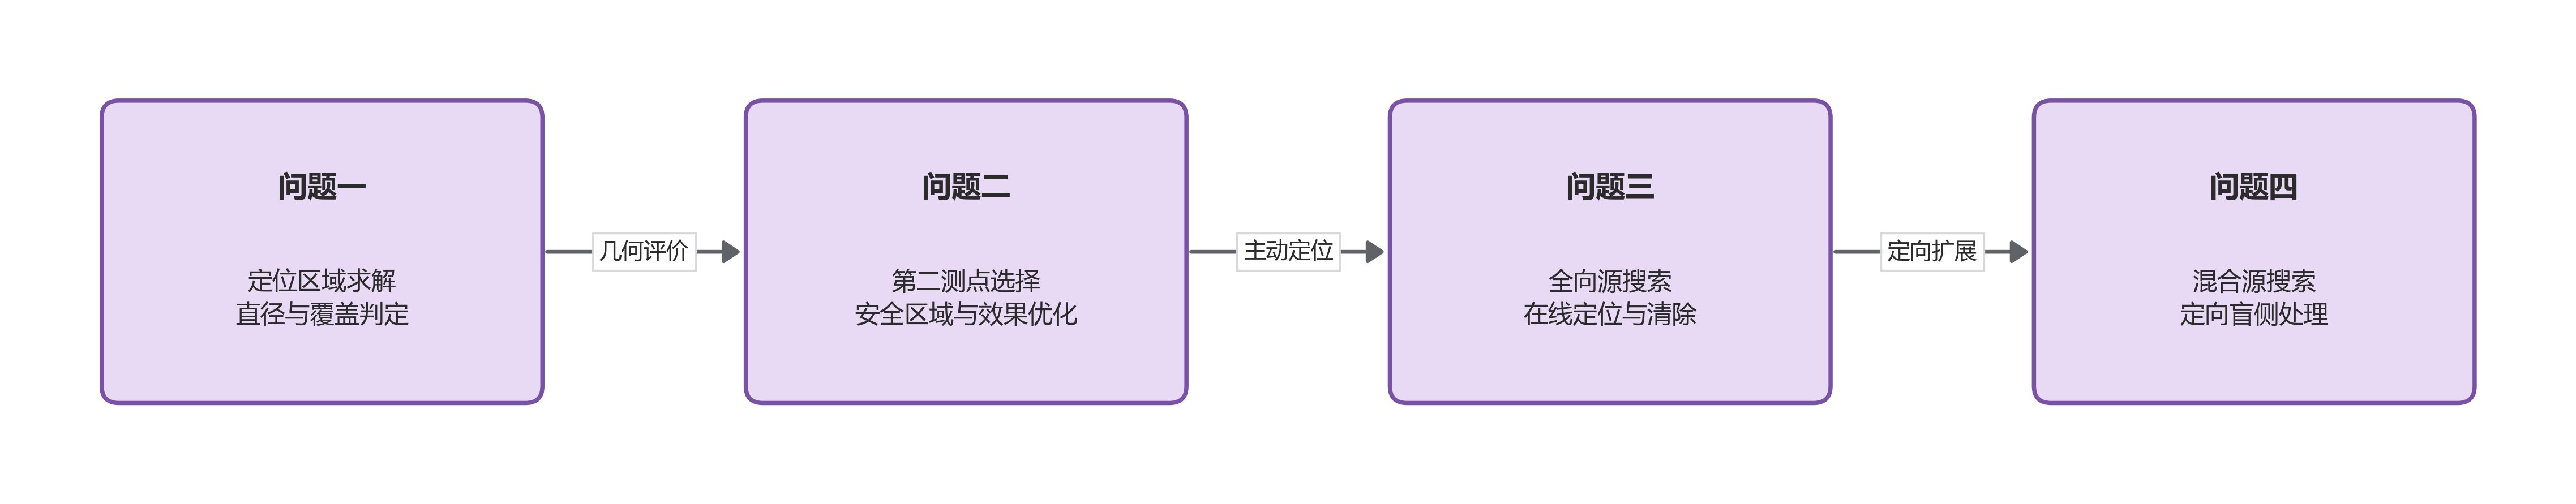
\includegraphics[width=0.98\linewidth]{images/fig_overall_flowchart.png}
    \caption{无线电干扰源定位与清除策略整体求解思路逻辑架构}
    \label{fig:overall_flowchart}
\end{figure}

\section{模型假设与符号说明}

\subsection{模型假设}
为使数学模型切合实际物理过程并保持数理严谨，本文提出如下合理假设：
\begin{enumerate}[leftmargin=2.5em, itemsep=0.15em]
    \item \textbf{目标位置静止与基准坐标无漂移}：目标干扰源在作业全过程中保持二维空间物理位置静止；机器狗自身定位与方位基准准确，坐标与航向角不存在系统漂移偏差。
    \item \textbf{信道频段相互正交与有效观测准入}：20 个离散频段相互独立无跨频互调干扰，同一信道在全域至多对应单一客观目标；各测站独立获取测向或无信号状态，仅当测站处于目标有效辐射半平面且距离不超过覆盖半径时产生有效示向角并参与多边形交会解算，无信号测站不作为正向测向约束。
    \item \textbf{测向角度物理误差严格有界}：测向仪的角度测量误差严格限制在闭区间 $[-\varepsilon, \varepsilon]$ 之内（误差半宽 $\varepsilon = 1^\circ$），不依赖先验概率分布假设，按极端最坏情况进行几何包络分析。
    \item \textbf{同点重复观测误差恒定}：在同一物理地点重复测向时，受固定的局部环境影响，测向系统误差保持不变，无法通过原地多次采样取平均来减小测向偏差。
    \item \textbf{分段匀速直线机动与离散动作执行}：机器狗转向、起步与制动过程极为迅速，近似为以 $5\text{ m/s}$ 固定速度运动的质点分段匀速直线机动；天线调谐、停靠测向、光学定位与激光清除等动作按离散事件串行执行并严格依规程累加时间；物理清除条件仅取决于与目标的真实欧氏间距（$\le 20\text{ m}$），不受目标辐射角度限制。
    \item \textbf{平坦地面视距传播与辐射源状态稳定}：电磁波在平坦二维地面内沿视距直线传播；目标干扰源在任务期间发射功率稳定且工作频率固定，全向源向全域各向同性辐射，定向源辐射主瓣朝向在任务期间固定不变，不存在动态旋转、跳频或间歇关机。
\end{enumerate}

\subsection{符号说明}
本文使用的主要数学符号及其物理意义如表 \ref{tab:symbols} 所示。

\begin{table}[htbp]
    \centering
    \small
    \caption{主要数学符号物理意义与数学定义说明}
    \label{tab:symbols}
    \begin{tabularx}{\linewidth}{c X c}
        \toprule[1.5pt]
        \textbf{符号} & \textbf{数学定义与物理意义} & \textbf{量纲 / 类型} \\
        \midrule
        $n$ & 参与协同交会定位的已知检测基站（观测点）总数 & 无量纲 (个) \\
        $\mathbf{p}_i$ & 第 $i$ 次观测时检测站的二维平面坐标，$\mathbf{p}_i = (x_i, y_i)^\top$ & $\text{m}$ \\
        $\hat\theta_i$ & 第 $i$ 次观测所得实测示向度（平面直角坐标系下逆时针度量的极角方向） & $\text{rad}$ / 度 \\
        $\varepsilon$ & 测向仪的客观物理误差确界半宽，$\varepsilon = 1^\circ = \pi/180\text{ rad}$ & $\text{rad}$ / 度 \\
        $\mathbf{s}$ & 未知的真实辐射源二维平面位置坐标，$\mathbf{s} = (s_x, s_y)^\top$ & $\text{m}$ \\
        $\mathcal{W}_i$ & 第 $i$ 次测向在空间中形成的前向有界角域（双向半平面的交集） & 平面闭子集 \\
        $\mathcal{R}$ & 全体有效协同观测共同约束下的联合交会定位区域（紧致凸多边形） & 紧致凸多边形 \\
        $\mathcal{V}$ & 定位凸多边形 $\mathcal{R}$ 逆时针有序排列的极点序列，$\mathcal{V} = \{\mathbf{v}_0, \dots, \mathbf{v}_{h-1}\}$ & 极点点列 \\
        $D$ & 定位多边形区域 $\mathcal{R}$ 内任意两点间欧氏距离的上确界（几何直径） & $\text{m}$ \\
        $(\mathbf{a}^*, \mathbf{b}^*)$ & 凸多边形上距离最远的一组极点对（直径端点对） & 极点坐标对 \\
        $\mathcal{C}^*$ & 以最远对踵极点对 $(\mathbf{a}^*, \mathbf{b}^*)$ 连线为直径构造的闭圆盘 & 平面闭圆盘 \\
        $\kappa$ & 直径圆盘 $\mathcal{C}^*$ 能否完全包含并覆盖定位区域 $\mathcal{R}$ 的布尔判定指标 & 布尔量 $\{0, 1\}$ \\
        \bottomrule[1.5pt]
    \end{tabularx}
\end{table}

\section{问题一：定位区域的直径与覆盖判定}

\subsection{问题分析}

问题一要求针对给定的若干检测点空间坐标及实测示向度，建立交会定位模型，设计求解定位多边形几何直径的具体算法，并判定以该直径构成的闭圆盘能否完全覆盖此定位区域。

求解问题一的核心难点在于：一方面，测向仪存在有界角度误差（$\pm 1^\circ$），需将离散的物理测向数据转化为严格的几何约束；另一方面，交会形成的多边形为连续闭合区域，无法直接通过离散网格采样来精确计算几何直径和判定圆盘覆盖。

为此，本文建立如下求解流程：
\[
    \{(\mathbf{p}_i, \hat\theta_i)\}_{i=1}^n \;\longrightarrow\; \{\mathcal{W}_i\}_{i=1}^n \;\longrightarrow\; \mathcal{V} \;\longrightarrow\; (D, \mathbf{a}^*, \mathbf{b}^*) \;\longrightarrow\; \kappa
\]
求解过程分为三个阶段。首先，根据测向误差确界将实测示向度转化为半平面约束，并通过求交得到定位多边形的有序极点序列。随后，利用凸分析极值原理证明区域直径必在极点处取得，通过旋转卡壳算法求取最远顶点对和区域几何直径。最后，以该点对连线为直径构造闭圆盘，并结合理论证明、正三角形几何反例和向量点积判据判断其覆盖性。

\subsection{模型建立}

\subsubsection{测向误差角域与半平面模型}

为实现上述交会定位与几何解算流程，首要环节是将物理测向数据转化为严密的几何约束。由于测向仪存在角度误差，单个检测点获得的观测不是一条理想射线，而是具有一定张角的扇形角域。因此，多站协同交会定位的本质是求取各测向角域在二维平面上的公共部分。为此，本节利用双向半平面刻画单个检测点的前向观测角域，进而将联合交会定位区域 $\mathcal{R}$ 严格表示为有限闭半平面的交集 \cite{gholami2013}，为后续多边形顶点解算与几何直径计算提供标准的不等式输入。

设参与协同交会定位的已知检测点数量为 $n$。对于第 $i$ 个检测点，其空间平面位置记为 $\mathbf{p}_i$，实测示向度记为 $\hat\theta_i$（$i=1, \dots, n$）。设真实辐射源的目标位置为 $\mathbf{s}$，其相对于检测点 $\mathbf{p}_i$ 的理论真值方位极角记为 $\theta_i^*$。在测向仪物理误差半宽 $\varepsilon = 1^\circ$ 的有界约束下，实测示向度与真实方位极角满足：
\begin{equation}
    \hat\theta_i \equiv \theta_i^* + e_i \pmod{2\pi}, \quad |e_i| \le \varepsilon
\end{equation}

为了消除传统斜率法在正切奇异角（$\pi/2$ 与 $3\pi/2$）处的数值发散，并统一处理极角 $0/2\pi$ 跨界周期性，定义第 $i$ 次观测在两侧误差边界处的临界单位导向向量：
\begin{equation}
    \mathbf{u}_i^- = \begin{bmatrix} \cos(\hat\theta_i - \varepsilon) \\ \sin(\hat\theta_i - \varepsilon) \end{bmatrix}, \quad
    \mathbf{u}_i^+ = \begin{bmatrix} \cos(\hat\theta_i + \varepsilon) \\ \sin(\hat\theta_i + \varepsilon) \end{bmatrix}
\end{equation}

定义平面向量叉积行列式算子 $\det(\mathbf{a},\mathbf{b}) = a_x b_y - a_y b_x$。当且仅当向量 $\mathbf{b}$ 处于 $\mathbf{a}$ 的逆时针左侧半平面时，$\det(\mathbf{a},\mathbf{b}) \ge 0$。第 $i$ 次测向所确立的前向闭合楔形角域 $\mathcal{W}_i$ 可严格表示为两个闭半平面的交集：
\begin{equation}
    \mathcal{W}_i = \left\{ \mathbf{x} \in \mathbb{R}^2 : \det(\mathbf{u}_i^-, \mathbf{x}-\mathbf{p}_i) \ge 0, \quad \det(\mathbf{x}-\mathbf{p}_i, \mathbf{u}_i^+) \ge 0 \right\}
\end{equation}

全体有效协同观测的公共交会定位多边形 $\mathcal{R}$ 为全体前向角域之交集：
\begin{equation}
    \mathcal{R} = \bigcap_{i=1}^{n} \mathcal{W}_i
\end{equation}
由于每个闭半平面均为凸集，有限凸集之交仍为凸集。在合理的多站交会基线配置下，$\mathcal{R}$ 为非空、有界的紧致凸多边形，且满足真实目标真值包含性 $\mathbf{s} \in \mathcal{R}$。

在模型边界的界定上，本问求解的定位区域 $\mathcal{R}$ 严格由各检测点的测向角域交会形成。发射覆盖半径（$1000\sim 1500\text{ m}$）、近场 5 米盲区和目标区域 1800 米圆边界共同决定测向信号能否被成功接收。本问已经给出获得有效示向度的检测点，因此后续交会定位只处理这些观测形成的半平面约束，不再引入先验圆弧进行二次裁剪，从而保持凸多边形几何结构的严整性与算法求解的准确性。至此，由全体测向角域共同界定的定位区域被严格表征为包含 $2n$ 条线性不等式的闭凸集系统。

\subsection{模型求解}

\subsubsection{半平面交与定位多边形求解}

上述闭半平面系统在代数上完备界定了目标可行域，但隐式线性不等式无法直接提供空间拓扑结构。为支撑后续几何直径度量与覆盖判定，需将其显式转换为逆时针严格排序的极点序列：
\begin{equation}
    \mathcal{R} = \{\mathbf{x} \in \mathbb{R}^2 : A\mathbf{x} \le \mathbf{b}\} = \operatorname{conv}(\mathcal{V}), \quad \mathcal{V} = \{\mathbf{v}_0, \mathbf{v}_1, \dots, \mathbf{v}_{h-1}\}
\end{equation}
本文采用基于双端队列的增量半平面求交算法。预处理阶段先提取全部 $2n$ 条有向边界的法向角并按极角排序，同时对同向平行边界仅保留约束最严格者。随后，利用双端队列维护当前可行区域的活动边界；每加入一个新半平面，若队头或队尾的相邻交点落入不可行侧，便执行相应的出队剪枝。完成全部半平面的遍历和闭合检验后，联立相邻边界方程得到逆时针严格排列的规范化极点序列 $\mathcal{V}$。该算法将连续区域求解转化为有限边界极点计算，时间复杂度为 $O(n\log n)$，空间复杂度为 $O(n)$。

\subsubsection{旋转卡壳法求解区域直径}

基于上述解出的外轮廓极点序列 $\mathcal{V}$，多边形定位区域 $\mathcal{R}$ 的几何直径 $D$ 严格定义为区域内任意两点间欧氏距离的上确界：
\begin{equation}
    D = \max_{\mathbf{x}, \mathbf{y} \in \mathcal{R}} \|\mathbf{x} - \mathbf{y}\|_2
\end{equation}
作为连续二维闭集，$\mathcal{R}$ 内包含无穷多个点，直接求解两点间最大间距属于连续极值优化问题。为实现确定性快速求解，关键在于将连续搜索降维至有限极点集合的离散比较。为此，本文给出并证明如下极值分布命题：

\noindent\textbf{命题 1（凸多边形直径端点必为顶点）}\quad 紧致凸多边形 $\mathcal{R}$ 的几何直径 $D$ 必在该多边形的某对极点（外轮廓顶点）之间取得，即：
\begin{equation}
    D = \max_{\mathbf{v}_j, \mathbf{v}_k \in \mathcal{V}} \|\mathbf{v}_j - \mathbf{v}_k\|_2
\end{equation}

\begin{cumcmproof}
任取区域内的任意两点 $\mathbf{x}, \mathbf{y} \in \mathcal{R}$。由凸多边形极点表示定理，两点可分别展开为全体极点集的凸组合：$\mathbf{x} = \sum_{j=0}^{h-1} \lambda_j \mathbf{v}_j$ 与 $\mathbf{y} = \sum_{k=0}^{h-1} \mu_k \mathbf{v}_k$，其中系数满足 $\lambda_j, \mu_k \ge 0$ 且 $\sum_j \lambda_j = \sum_k \mu_k = 1$。利用系数归一性 $\sum_k \mu_k = \sum_j \lambda_j = 1$ 将差向量改写为双重凸组合，并由范数三角不等式放缩：
\begin{equation}
    \|\mathbf{x} - \mathbf{y}\|_2 = \left\| \sum_{j=0}^{h-1}\sum_{k=0}^{h-1} \lambda_j \mu_k (\mathbf{v}_j - \mathbf{v}_k) \right\|_2 
    \le \sum_{j=0}^{h-1}\sum_{k=0}^{h-1} \lambda_j \mu_k \|\mathbf{v}_j - \mathbf{v}_k\|_2 
    \le \max_{0 \le j, k \le h-1} \|\mathbf{v}_j - \mathbf{v}_k\|_2
\end{equation}
由于双重凸组合系数满足 $\sum_{j=0}^{h-1}\sum_{k=0}^{h-1} \lambda_j \mu_k = 1$，连续区域内任意两点间的欧氏间距上界必不超过有限极点对间的最大距离；又由极点包含性 $\mathcal{V} \subset \mathcal{R}$，该极大值在极点集上严格可达，证毕。
\end{cumcmproof}

命题 1 将连续搜索降维至 $\binom{h}{2}$ 对离散顶点比较，但全顶点穷举计算复杂度仍为 $O(h^2)$。根据对踵几何特征，两点最大间距必在相互平行的外切支撑线接触点（对踵点对）处取得。为此引入旋转卡壳算法 \cite{toussaint1983}，通过一对平行卡尺绕多边形旋转步进，仅需在 $O(h)$ 线性时间内遍历全部对踵候选，即可精确提取区域几何直径 $D$ 及最远顶点对 $(\mathbf{a}^*, \mathbf{b}^*)$。

\subsubsection{直径圆盘覆盖判定}

求得几何直径 $D$ 与最远极点对 $(\mathbf{a}^*, \mathbf{b}^*)$ 后，针对以最远点连线为直径构造的闭圆盘（圆心 $\mathbf{c}^* = \frac{\mathbf{a}^* + \mathbf{b}^*}{2}$，半径 $R = D/2$）：
\begin{equation}
    \mathcal{C}^* = \left\{ \mathbf{x} \in \mathbb{R}^2 : \|\mathbf{x} - \mathbf{c}^*\|_2 \le \frac{D}{2} \right\}
\end{equation}
直觉常误以为直径既然是区域内最大间距，该圆盘便理应包含多边形全部点。然而基于平面凸多边形的包含几何理论 \cite{welzl1991}，严密分析表明：\textbf{以最远点间距为直径构造的闭圆盘，并不能恒定保证完全覆盖定位多边形。}

构造理论反例予以证明：设交会定位区域为边长为 $D$ 的正三角形 $\triangle ABC$。由正三角形几何性质可知，其任意两点间距离的最大值即为边长，故该凸多边形的几何直径为 $D$。若取底边端点 $A, B$ 作为最远点对构造闭圆盘 $\mathcal{C}^*$，圆心为其几何中点 $\mathbf{c}^* = (\mathbf{v}_A + \mathbf{v}_B)/2$，半径 $R = 0.5D$。第三个顶点 $C$ 到圆心 $\mathbf{c}^*$ 的距离为该三角形的高：
\begin{equation}
    h_{\triangle} = \|\mathbf{v}_C - \mathbf{c}^*\|_2 = \frac{\sqrt{3}}{2} D \approx 0.8660 D > 0.5 D
\end{equation}
顶点 $C$ 位于该圆盘之外（超出圆盘边界达 $0.366D$），否定了恒能完全覆盖的假设。根据几何学荣格定理，平面上直径为 $D$ 的任意有界闭集，其最小覆盖圆半径满足 $R_{\min} \le \frac{\sqrt{3}}{3} D \approx 0.5774 D$。而以最远点间距构造的圆盘半径仅为 $0.5D < 0.5774D$。因此，当多边形在垂直于直径的方向上横向宽展较大时，其顶点便会超出该圆盘。

为判定具体多边形的覆盖性，利用凸集性质，多边形 $\mathcal{R} = \operatorname{conv}(\mathcal{V})$ 被闭圆盘完全包含充要等价于全体极点落入圆盘内部。借助向量点积恒等式：
\begin{equation}
    (\mathbf{x} - \mathbf{a}^*) \cdot (\mathbf{x} - \mathbf{b}^*) = \|\mathbf{x} - \mathbf{c}^*\|_2^2 - \frac{D^2}{4}
\end{equation}
点 $\mathbf{x} \in \mathcal{C}^* \iff (\mathbf{x} - \mathbf{a}^*) \cdot (\mathbf{x} - \mathbf{b}^*) \le 0$。该式将开方几何距离检验转化为无需开方的线性内积符号判据，避免了浮点舍入误差。据此定义覆盖布尔算子 $\kappa \in \{0, 1\}$：
\begin{equation}
    \kappa = 
    \begin{cases}
        1, & \text{若 } \forall \mathbf{v}_j \in \mathcal{V},\; (\mathbf{v}_j - \mathbf{a}^*) \cdot (\mathbf{v}_j - \mathbf{b}^*) \le 0 \\
        0, & \text{若 } \exists \mathbf{v}_j \in \mathcal{V},\; (\mathbf{v}_j - \mathbf{a}^*) \cdot (\mathbf{v}_j - \mathbf{b}^*) > 0
    \end{cases}
\end{equation}
若 $\kappa=0$，记录超出圆盘边界的最大超量 $g_{\text{viol}} = \max_j \max\{(\mathbf{v}_j - \mathbf{a}^*) \cdot (\mathbf{v}_j - \mathbf{b}^*), 0\}$ 及其对应越界顶点。至此，从测向数据到定位多边形、几何直径求解以及圆盘覆盖判定的完整几何机制如图 \ref{fig:q1_dual_panel} 所示。其中图 \ref{fig:q1_dual_panel}(a) 直观展示了多站测向角域求交围成的定位多边形；图 \ref{fig:q1_dual_panel}(b) 说明了利用旋转卡壳法在对踵平行外切线上提取区域直径与构造直径圆盘的过程；图 \ref{fig:q1_dual_panel}(c) 则清晰刻画了正三角形底边直径圆盘无法覆盖对向顶点的理论反例与越界几何形态。

\begin{figure}[htbp]
    \centering
    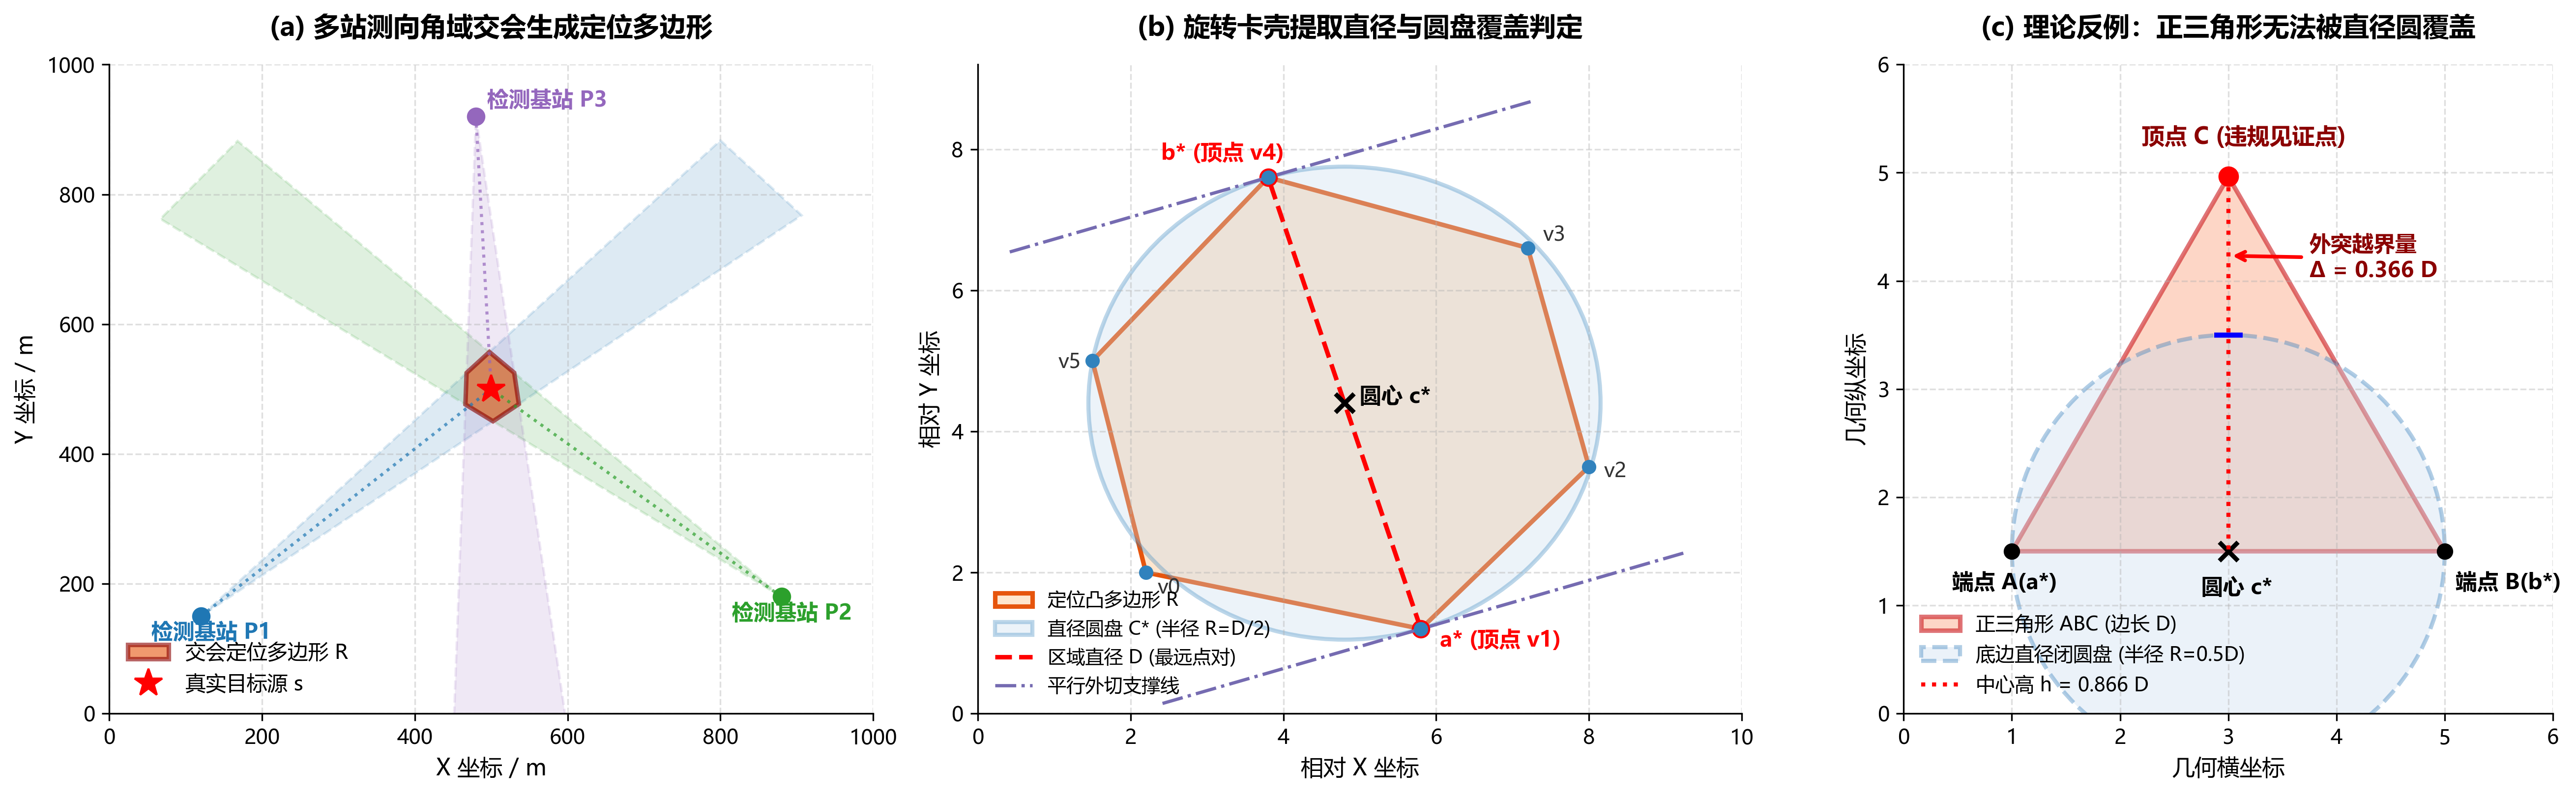
\includegraphics[width=0.96\textwidth]{images/fig_q1_dual_panel.png}
    \caption{多站测向角域交会、定位多边形直径提取与圆盘覆盖判定几何机制示意图}
    \label{fig:q1_dual_panel}
\end{figure}

\subsection{结果分析与模型检验}

为检验上述交会定位模型、几何直径算法与覆盖判定准则的正确性与数值稳定性，本节首先通过典型四站对称基准算例与大规模蒙特卡洛统计展示解算过程与覆盖特性规律，随后设计独立的几何枚举对照算法开展多重独立交叉复核与极端工况压力测试，最后分析计算复杂度与异常几何输入的自适应处理机制。

\subsubsection{基准算例与覆盖特性分析}

为检验算法的基本执行流程与数值精度，首先选取四向对称测向基准算例进行解算。4 个观测站环绕分布于半径 $1000\text{ m}$ 的圆周上：$\mathbf{p}_1=(1000, 0)\text{ m}$、$\mathbf{p}_2=(0, 1000)\text{ m}$、$\mathbf{p}_3=(-1000, 0)\text{ m}$、$\mathbf{p}_4=(0, -1000)\text{ m}$，实测示向度分别为指向坐标原点的正四向极角 $180^\circ, 270^\circ, 0^\circ, 90^\circ$。在误差半宽 $\varepsilon = 1^\circ$ 约束下，共形成 8 条半平面边界。

算法解算得到严格中心对称的正规凸八边形，覆盖面积为 $1197.81\text{ m}^2$。旋转卡壳算法求得其最大几何直径为 $D = 48.523\text{ m}$，对应最远顶点对坐标为 $(17.156, -17.156)\text{ m}$ 与 $(-17.156, 17.156)\text{ m}$。以该点对连线为直径构造闭圆盘（圆心为坐标原点，半径 $24.262\text{ m}$），经逐顶点点积检验，各顶点的最大点积超量仅为 $9.64 \times 10^{-12}\text{ m}^2$，低于预设数值容差，覆盖指标输出 $\kappa = 1$，实现了对定位多边形的完全覆盖。基准算例解算指标汇总于表 \ref{tab:q1_default_results}。

\begin{table}[htbp]
    \centering
    \small
    \caption{Q1 默认基准算例（四站对称观测）几何解算结果表}
    \label{tab:q1_default_results}
    \renewcommand{\arraystretch}{1.08}
    \begin{tabularx}{\linewidth}{X c c c X}
        \toprule[1.5pt]
        \textbf{几何参数 / 评估指标} & \textbf{符号 / 变量} & \textbf{数值结果} & \textbf{量纲} & \textbf{验证状态与备注} \\
        \midrule
        观测基站总数 & $N_{\text{obs}}$ & 4 & 个 & 环绕分布于 $R=1000\text{ m}$ \\
        有效半平面约束数 & $M$ & 8 & 条 & 每站提供 $\pm 1^\circ$ 双向边界 \\
        定位区域状态 & $\text{Status}$ & 正常有界 & - & 严格有界、正常非退化凸多边形 \\
        多边形极点总数 & $h$ & 8 & 个 & 严格逆时针拓扑排序 \\
        定位多边形覆盖面积 & $S$ & 1197.81 & $\text{m}^2$ & 对称八边形紧致闭包 \\
        定位区域最大几何直径 & $D$ & \textbf{48.523} & $\text{m}$ & 旋转卡壳提取，最远对 $(\mathbf{a}^*, \mathbf{b}^*)$ \\
        直径圆盘圆心坐标 & $\mathbf{c}^*$ & $(0.000, 0.000)$ & $\text{m}$ & 最远点对连线几何中点 \\
        直径圆盘半径 & $R = D/2$ & 24.262 & $\text{m}$ & 待检圆盘半径 \\
        逐顶点点积最大违规量 & $g_{\text{viol}}$ & $9.64 \times 10^{-12}$ & $\text{m}^2$ & 低于预设容差 $10^{-10}$，按零处理 \\
        圆盘完全覆盖判定结论 & $\kappa$ & \textbf{完全覆盖} & - & 默认基准算例下圆盘实现 $100\%$ 覆盖 \\
        \bottomrule[1.5pt]
    \end{tabularx}
\end{table}

上述基准算例表明，在空间高度对称的测向环境下，几何直径构造的圆盘确实能够实现对定位多边形的完全覆盖。然而，在非对称或任意多站协同的普遍场景下，该结论是否仍恒定成立？为从大样本统计层面检验前述理论反例的实证表现，本文基于固定随机种子（\texttt{20260911}）进一步生成 1000 组随机蒙特卡洛测试样本，定义各算例中凸多边形顶点相对直径圆盘边界的最大相对半径超量：
\begin{equation}
    \Delta_{\mathrm{rel}} = \frac{\max_j \|\mathbf{v}_j - \mathbf{c}^*\|_2 - D/2}{D/2} \times 100\%
\end{equation}
当 $\Delta_{\mathrm{rel}} \le 0$ 时表示多边形完全落入圆盘内（$\kappa=1$）；当 $\Delta_{\mathrm{rel}} > 0$ 时表示存在顶点超出圆盘边界（$\kappa=0$）。

在 1000 个随机蒙特卡洛测试样本中，共有 347 个算例被直径圆盘完全覆盖（占 $34.7\%$），653 个算例发生外突未被完全覆盖（占 $65.3\%$）。图 \ref{fig:q1_validation} 绘制了将 1000 个算例按相对半径超量由小到大升序排序后的经验分布曲线。

\begin{figure}[htbp]
    \centering
    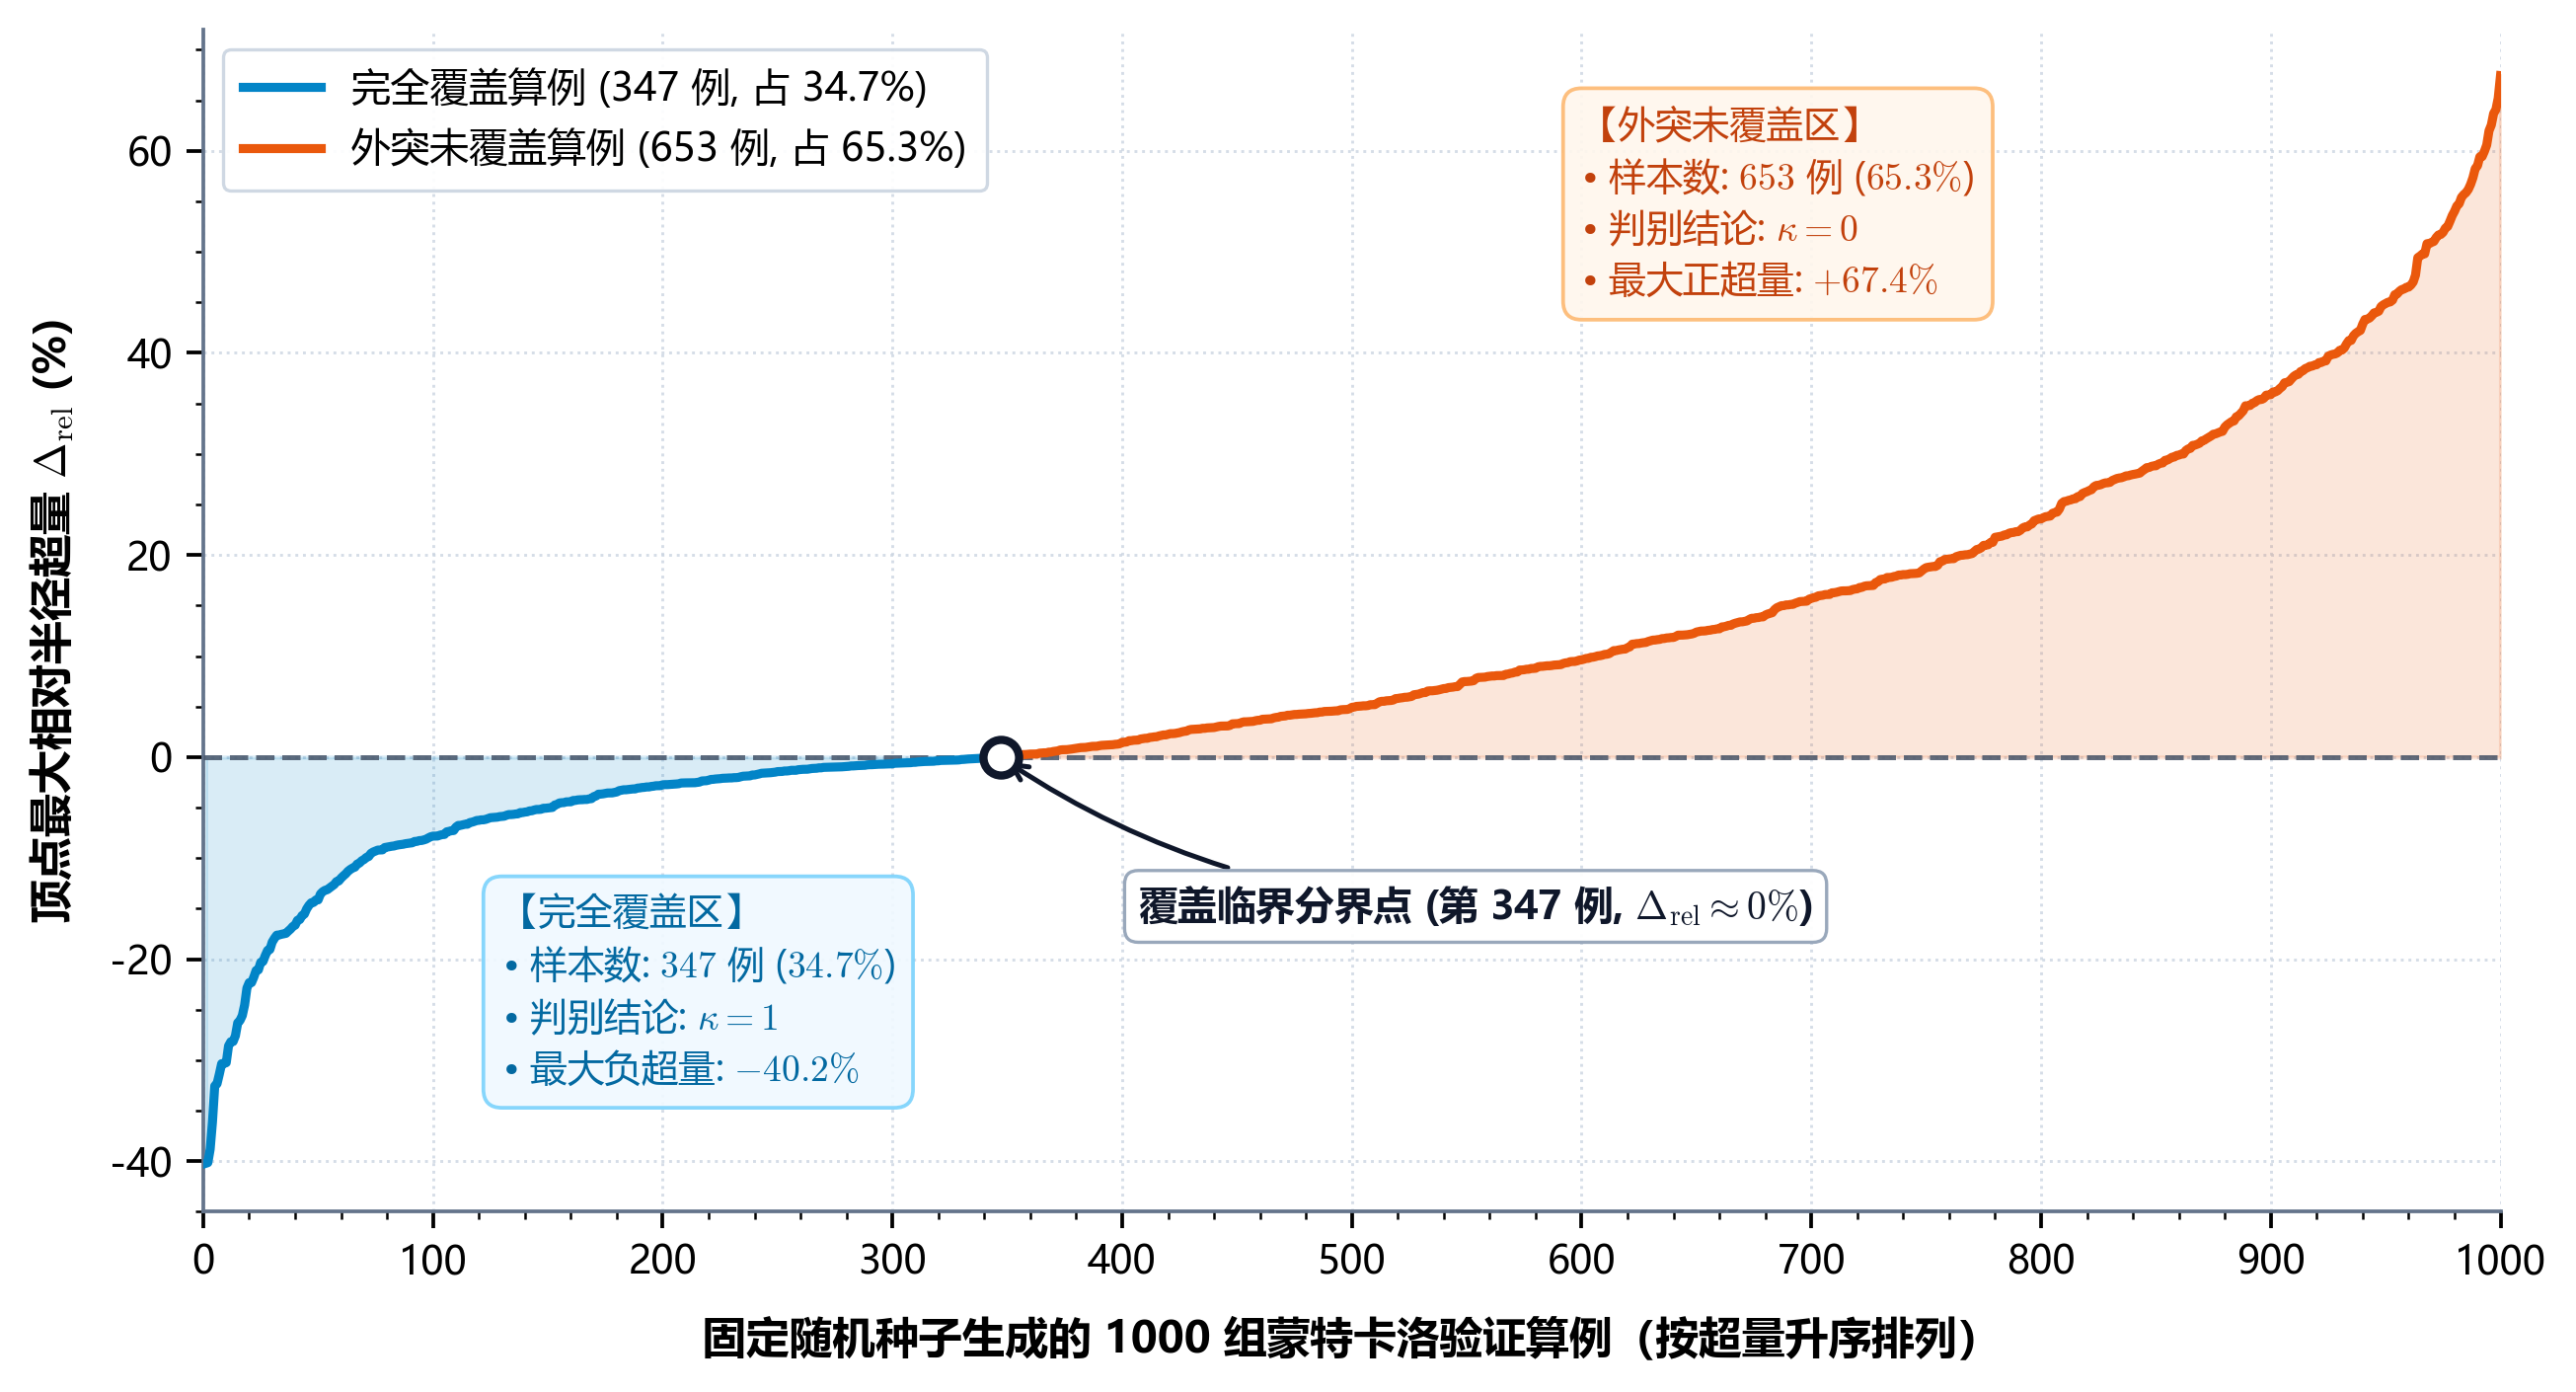
\includegraphics[width=0.76\linewidth]{images/q1_validation.png}
    \vspace{-0.5em}
    \caption{固定随机种子生成的 1000 个随机蒙特卡洛算例相对半径超量排序经验折线}
    \label{fig:q1_validation}
    \vspace{-0.5em}
\end{figure}

由图 \ref{fig:q1_validation} 可见，曲线自负超量区跨越零点延伸至正超量区（最大正超量为 $+67.4\%$）。这直观表明多边形能否被其直径圆盘覆盖取决于横向宽展程度：当多边形在垂直于直径方向较窄时容易被圆盘包含；而当形态趋近于正三角形或宽展钝角几何时，顶点便易超出圆盘。该统计实证与理论反例互相印证，证明了算法对覆盖成立与外突失效均具备灵敏准确的双向判别能力。

\subsubsection{算法对照与稳健性检验}

在明确了基准算例数值与千例统计规律之后，为检验增量半平面交与旋转卡壳主算法在浮点计算与边界剪枝中是否存在潜在偏差，本文专门设计了一套基于穷举原理的独立对照复核算法，针对三个核心求解环节展开多角度独立交叉校验：
\begin{enumerate}[leftmargin=2.5em, itemsep=0.2em]
    \item \textbf{多边形构造对照（全边界两两求交与可行性筛选法）：}不同于主算法依赖极角排序与双端队列动态维护外轮廓，对照算法直接对全体 $2n$ 条半平面边界直线进行全组合联立求解，解出全部 $\binom{2n}{2}$ 个候选交点坐标；随后将每个交点逐一代入全部 $2n$ 个半平面不等式中检验可行性，剔除所有违反任意约束的外侧交点，仅保留全局可行顶点；最后对保留的离散点集执行平面凸包构建，得到无冗余的逆时针多边形顶点集。该方法计算复杂度为 $O(n^3)$，但逻辑直观、不涉及增量剪枝，可作为多边形顶点的可靠对照依据。
    \item \textbf{几何直径求解对照（全顶点对欧氏距离全局穷举法）：}不依赖旋转切线步进与对踵点候选理论，对照算法直接对多边形的全部 $h$ 个顶点展开全局双重循环穷举，计算任意两顶点间的欧氏距离：$D_{\text{ref}} = \max_{0 \le j < k < h} \|\mathbf{v}_j - \mathbf{v}_k\|_2$。该方法复杂度为 $O(h^2)$，遍历全部顶点组合，用于直接检验旋转卡壳算法在对踵点搜索时是否存在漏检或步进跳跃。
    \item \textbf{圆盘覆盖判定对照（顶点外接欧氏半径直接比对法）：}对照算法绕过向量点积代数式，直接计算每个多边形顶点到直径圆心 $\mathbf{c}^* = (\mathbf{a}^* + \mathbf{b}^*)/2$ 的实际欧氏空间距离 $d_j = \|\mathbf{v}_j - \mathbf{c}^*\|_2$。当且仅当所有顶点均满足 $d_j \le D/2 + 10^{-10}\text{ m}$ 时判定为完全覆盖，与主算法的点积准则形成机理独立的对照。
\end{enumerate}

在 1000 组多站协同测向测试算例的全量对照比对中：增量半平面交与全边界两两筛选法求得的多边形极点序列完全一致，面积相对偏差小于 $10^{-12}$；旋转卡壳算法与全点对距离穷举法求得的几何直径绝对偏差严格为 $0.0\text{ m}$；点积判据与欧氏半径判据对圆盘覆盖性的布尔判断结果一致率达 $100\%$。

本文进一步开展五项极端工况下的稳健性压力测试。对观测顺序进行 1000 次随机置换，并人工添加 1000 次同向完全重合半平面后，算法均能自适应处理，输出保持不变。对整个系统施加 $37^\circ$ 空间旋转和大距离平移时，求解区域直径同样严格保持。8443 次增量约束测试均满足定位区域直径单调非增性质；将临界容差调整为 $10^{-9}$ 和 $10^{-11}$ 时，求解状态与覆盖判定也保持高度稳定。双算法对照与稳健性检验结果汇总于表 \ref{tab:q1_verification_methods}。

\begin{table}[!ht]
    \centering
    \small
    \caption{主算法与复核方法对照及大规模检验统计表}
    \label{tab:q1_verification_methods}
    \renewcommand{\arraystretch}{1.08}
    \begin{tabularx}{\linewidth}{>{\raggedright\arraybackslash}p{2.6cm} X X c >{\raggedright\arraybackslash}p{3.0cm}}
        \toprule[1.5pt]
        \textbf{计算环节 / 检验项目} & \textbf{正式算法} & \textbf{对照复核方法 / 检验标准} & \textbf{样本规模} & \textbf{检验结论 / 通过率} \\
        \midrule
        定位多边形构造 & 极角排序半平面交 ($O(n\log n)$) & 边界两两求交全筛选 ($O(n^3)$) & 1000 例 & 极点集与面积 100\% 一致 \\
        区域几何直径计算 & 旋转卡壳算法 ($O(h)$) & 全顶点对距离穷举 ($O(h^2)$) & 1000 例 & 直径绝对偏差严格为 $0.0\text{ m}$ \\
        直径圆盘覆盖判定 & 顶点向量点积准则 ($O(h)$) & 顶点到圆心欧氏距离准则 ($O(h)$) & 1000 例 & 覆盖布尔值 100\% 一致 \\
        观测序列乱序不变性 & 随机置换观测输入顺序 & 比较置换前后求解直径与覆盖 & 1000 次 & 1000 次全部通过 ($\Delta D = 0.0\text{ m}$) \\
        冗余约束不变性检验 & 人工添加同向完全重合半平面 & 比较添加前后几何输出 & 1000 次 & 1000 次全部通过 (完全一致) \\
        刚体空间变换不变性 & $37^\circ$ 旋转 + 大距离平移 & 比较变换前后区域直径 & 100 次 & 100 次全部通过 (严格保持) \\
        约束增加单调性检验 & 逐步递增有效观测半平面 & 验证几何区域直径单调非增 & 8443 次 & \textbf{8443 次检验 100\% 通过} \\
        容差数值敏感性检验 & 临界容差 $10^{-9}$ 与 $10^{-11}$ & 检验求解状态与覆盖分类稳定度 & 50 次 & 50 次全部通过 (数值高度稳定) \\
        算法综合执行效率 & 正式算法 + 双算法对照复核 & 包含全部复核的千例总耗时 & 1000 例 & 总耗时 3.24 s (单例 3.24 ms) \\
        \bottomrule[1.5pt]
    \end{tabularx}
\end{table}

\subsubsection{复杂度与异常情形分析}

在算法复杂度与工程可用性方面：常规运行模式下仅执行增量半平面交与旋转卡壳算法，理论时间复杂度为 $O(n\log n)$，空间复杂度为 $O(n)$；在标准运行环境下，包含全套对照复核的 1000 例测试平均单例耗时仅为 3.24 毫秒，计算效率充分满足工程实时应用需求。同时，算法设计了针对空集、无界可行域、退化线段或单点等异常几何输入的自适应状态判别机制，仅在正常凸多边形状态下输出确定性几何直径与覆盖结论，为后续选点优化与机动搜索策略提供了底层计算支持。

\section{问题二：第二检测点选择与候选区域}

\subsection{问题分析}

在问题二中，机器狗在第一检测点 $\mathbf{p}_1$ 测得某干扰源的初始示向度 $\hat\theta_1$。题设要求确定第二检测点 $\mathbf{p}_2$ 的选择策略与较优候选区域。基于问题一所建立的测向角域半平面交会模型与多边形几何直径解算算法，第二检测点的选择需兼顾以下两点：
\begin{enumerate}[leftmargin=2.5em, itemsep=0.2em]
    \item \textbf{信号接收保证：}干扰源覆盖半径 $R \in [1000, 1500]\text{ m}$ 未知。为获得不依赖未知实际覆盖半径的确定性接收保证，本文选取如下充分安全条件：第二检测点到该干扰源所有相容位置的距离均不得超过最小覆盖半径 $R_{\min} = 1000\text{ m}$。
    \item \textbf{定位效果最优：}在目标先验分布未知的情况下，以两次交会后最坏情况下的定位多边形几何直径衡量定位效果，采用极小化极大（Min-Max）准则使该最差后验直径达到最小 \cite{tokekar2013}。
\end{enumerate}

选点以两次交会后的最坏后验定位效果为主目标，并将移动距离与安全余量作为次级优化准则。

\subsection{模型建立}

\subsubsection{初次观测后的目标可行域}

设第一检测点坐标为 $\mathbf{p}_1 = (x_1, y_1)^\top$，实测示向度为 $\hat\theta_1$。初次观测后，干扰源真实位置 $\mathbf{s}$ 满足如下几何约束系统：
\begin{equation}
    \begin{cases}
        \mathbf{s} \in \mathcal{W}(\mathbf{p}_1, \hat\theta_1, \varepsilon) & (\text{测向角域约束，误差半宽 }\varepsilon = 1^\circ) \\
        \|\mathbf{s} - \mathbf{p}_1\|_2 \le R_{\max} = 1500\text{ m} & (\text{信号有效接收覆盖半径约束}) \\
        \|\mathbf{s}\|_2 \le R_{\text{target}} = 1800\text{ m} & (\text{目标分布圆形区域约束}) \\
        \|\mathbf{s} - \mathbf{p}_1\|_2 > r_{\text{near}} = 5\text{ m} & (\text{近场强信号盲区排除约束})
    \end{cases}
\end{equation}

上述约束的交集即为初测后的目标可行域 $\mathcal{P}_1$。为便于计算，采用角域射线与圆边界切线构建包含 $\mathcal{P}_1$ 的凸多边形外包络 $\mathcal{P}_1^+$（满足 $\mathcal{P}_1 \subseteq \mathcal{P}_1^+$）。数值实现中，目标圆区域及最大接收圆均采用 48 边外切正多边形近似，以保证 $\mathcal{P}_1 \subseteq \mathcal{P}_1^+$ 的包含关系。在基准算例（$\mathbf{p}_1 = (0, 0)\text{ m}, \hat\theta_1 = 0^\circ$）下，$\mathcal{P}_1^+$ 为底边长 $52.36\text{ m}$、高 $1500\text{ m}$ 的等腰三角形。

\subsubsection{第二检测点的安全候选域}

为保证在第二检测点 $\mathbf{p}_2$ 处必定接收到信号，定义信号接收安全余量：
\begin{equation}
    m(\mathbf{p}_2) = R_{\min} - \max_{\mathbf{s} \in \mathcal{P}_1^+} \|\mathbf{p}_2 - \mathbf{s}\|_2
\end{equation}

若考虑定位与控制误差，可设置缓冲距离 $b > 0$ 要求 $m(\mathbf{p}_2) \ge b$；本文基准模型取 $b = 0$。

由于欧氏距离关于点 $\mathbf{s}$ 具有凸性，点 $\mathbf{p}_2$ 到凸多边形 $\mathcal{P}_1^+$ 内任意点的最大距离必在其有限顶点集 $V(\mathcal{P}_1^+)$ 处取得：
\begin{equation}
    \max_{\mathbf{s} \in \mathcal{P}_1^+} \|\mathbf{p}_2 - \mathbf{s}\|_2 = \max_{\mathbf{v} \in V(\mathcal{P}_1^+)} \|\mathbf{p}_2 - \mathbf{v}\|_2
\end{equation}
据此，第二检测点的保守安全候选区域 $\mathcal{U}$ 为：
\begin{equation}
    \mathcal{U} = \left( \bigcap_{\mathbf{v} \in V(\mathcal{P}_1^+)} \left\{ \mathbf{p}_2 \in \mathbb{R}^2 : \|\mathbf{p}_2 - \mathbf{v}\|_2 \le R_{\min} \right\} \right) \setminus \{\mathbf{p}_1\}
\end{equation}
即 $\mathcal{U}$ 为以 $\mathcal{P}_1^+$ 各顶点为圆心、$R_{\min}$ 为半径的闭圆盘交集并排除第一检测点自身。排除 $\mathbf{p}_1$ 是由于题设同地点重复检测的环境误差保持不变，原地再次测量无法提供独立测向基线。只要 $\mathbf{p}_2 \in \mathcal{U}$，即可确保对可行域内的任意源位置均处于有效接收范围内。若 $\mathcal{U} = \varnothing$，表明在以 $R_{\min}$ 为充分安全约束下无可行测点，算法将给出无解标识并转入回退流程。

\subsubsection{第二检测点优化模型}

在安全区域 $\mathcal{U}$ 内，机器狗在 $\mathbf{p}_2$ 处观测可能出现两种情形：
\begin{enumerate}[leftmargin=2.5em, itemsep=0.2em]
    \item 若第二检测点距干扰源真实位置不超过近场阈值（$\|\mathbf{p}_2 - \mathbf{s}\|_2 \le r_{\text{near}} = 5\text{ m}$），测向接口返回 \texttt{near}。机器狗随后可进入光学精确定位与清除流程，因此在第二测点选择目标中将该反馈视为终止分支，令其剩余位置不确定性为 $0$；
    \item 若处于近场之外，测得示向度 $\hat\theta_2$。在测向误差 $e_2 \in [-\varepsilon, \varepsilon]$ 作用下，形成第二角域 $\mathcal{W}_2$，交会后的保守后验可行域为 $\mathcal{P}_2 = \mathcal{P}_1^+ \cap \mathcal{W}_2$。
\end{enumerate}

据此，定义单次观测下的后验定位损失函数为：
\begin{equation}
    L(\mathbf{p}_2; \mathbf{s}, e) = \begin{cases}
        0, & \|\mathbf{p}_2 - \mathbf{s}\|_2 \le r_{\text{near}} \\
        \operatorname{diam}\left[ \mathcal{P}_1^+ \cap \mathcal{W}\left(\mathbf{p}_2, \operatorname{bearing}(\mathbf{p}_2, \mathbf{s}) + e, \varepsilon\right) \right], & \|\mathbf{p}_2 - \mathbf{s}\|_2 > r_{\text{near}}
    \end{cases}
\end{equation}
在连续理论上，真实相容状态属于 $\mathcal{P}_1$。为保守覆盖源位置趋近 5 米盲区边界时的极限情形，连续评估将状态集合扩展至闭包 $\overline{\mathcal{P}}_1 = \operatorname{cl}(\mathcal{P}_1)$，数值采样点集相应满足 $S_N \subseteq \overline{\mathcal{P}}_1$。交会区域采用外包络 $\mathcal{P}_1^+$ 实施保守估计，定义保守最坏后验直径为：
\begin{equation}
    J^+(\mathbf{p}_2) = \sup_{\mathbf{s} \in \overline{\mathcal{P}}_1,\; |e| \le \varepsilon} L(\mathbf{p}_2; \mathbf{s}, e)
\end{equation}
式中明确区分了真实源状态空间 $\mathbf{s} \in \overline{\mathcal{P}}_1$ 与保守包络几何 $\mathcal{P}_1^+$。在数值解算时，采用有限采样集（$N$ 个代表源状态 $S_N \subset \overline{\mathcal{P}}_1$ 与 $M$ 个误差节点 $E_M$）计算离散评估指标：
\begin{equation}
    \widehat{J}_{N,M}(\mathbf{p}_2) = \max_{\mathbf{s}_i \in S_N,\; e_j \in E_M} L(\mathbf{p}_2; \mathbf{s}_i, e_j)
\end{equation}

经全域粗筛与局部寻优后，入围候选点进入精细评估阶段（$N=64, M=7$）。设进入精细评估的候选点集合为 $\mathcal{Q}_{\text{final}} \subset \mathcal{U}$，当前优化搜索求得的最优评价值与数值推荐点定义为：
\begin{equation}
    \widetilde{J}_{64,7} = \min_{\mathbf{p} \in \mathcal{Q}_{\text{final}}} \widehat{J}_{64,7}(\mathbf{p}), \qquad \widetilde{\mathbf{p}}_2 \in \arg\min_{\mathbf{p} \in \mathcal{Q}_{\text{final}}} \widehat{J}_{64,7}(\mathbf{p})
\end{equation}
进入精细评估阶段的候选点按 $(\widehat{J}_{64,7}(\mathbf{p}), \|\mathbf{p} - \mathbf{p}_1\|_2, -m(\mathbf{p}))$ 的字典序严格排序并优选。

为进一步量化给出较优候选区域，定义在空间采样网格 $\mathcal{G}_h$（网格步长 $h$）上相对容差 $\tau > 0$（如 $\tau = 1\%, 3\%, 5\%$）的近优候选区域：
\begin{equation}
    \widehat{\mathcal{C}}_{\tau, h} = \left\{ \mathbf{p} \in \mathcal{G}_h \cap \mathcal{U} : \widehat{J}_{N,M}(\mathbf{p}) \le (1+\tau)\widehat{J}_{N,M, h}^* \right\}
\end{equation}
式中 $\widehat{J}_{N,M, h}^* = \min_{\mathbf{p} \in \mathcal{G}_h \cap \mathcal{U}} \widehat{J}_{N,M}(\mathbf{p})$ 为全域网格扫描下的基准最优值。该区域给出了在定位性能损失受控前提下允许选点的几何范围。

\subsection{模型求解}

\subsubsection{分层搜索与精细评估}

为兼顾全局搜索视野与计算效率，采用全域粗筛、局部寻优与精细评估三阶段求解算法：
\begin{enumerate}[leftmargin=2.5em, itemsep=0.2em]
    \item \textbf{全域粗筛：}以 $\mathcal{P}_1^+$ 的最小包围圆（半径记为 $r_{\mathrm{MEC}}$）圆心为基准向四周引出 12 个辐射方向，分别在安全射线最大长度的 $55\%$ 与 $90\%$ 处取样，连同圆心共生成至多 25 个初选候选点，并采用 24 个源点 $\times$ 3 个误差节点（$-\varepsilon, 0, \varepsilon$）进行粗评估；
    \item \textbf{局部寻优：}选取粗筛前 3 个种子点，以初始步长 $h_0 = \min\{200, \max[20, 0.45(R_{\min}-r_{\mathrm{MEC}})]\}\text{ m}$ 进行 4 轮八邻域步长折半搜索；
    \item \textbf{精细评估：}将粗筛前 6 点与局部寻优点合并去重构建最终入围集 $\mathcal{Q}_{\text{final}}$，采用 64 个源点 $\times$ 7 个误差节点实施最终离散复核，输出字典序排序前三的优质候选点，并以首位点作为基准推荐点 $\widetilde{\mathbf{p}}_2$。
\end{enumerate}

第二检测点三阶段快速筛选与优化流程如图 \ref{fig:q2_flowchart} 所示。

\begin{figure}[htbp]
    \centering
    \vspace{0.2em}
    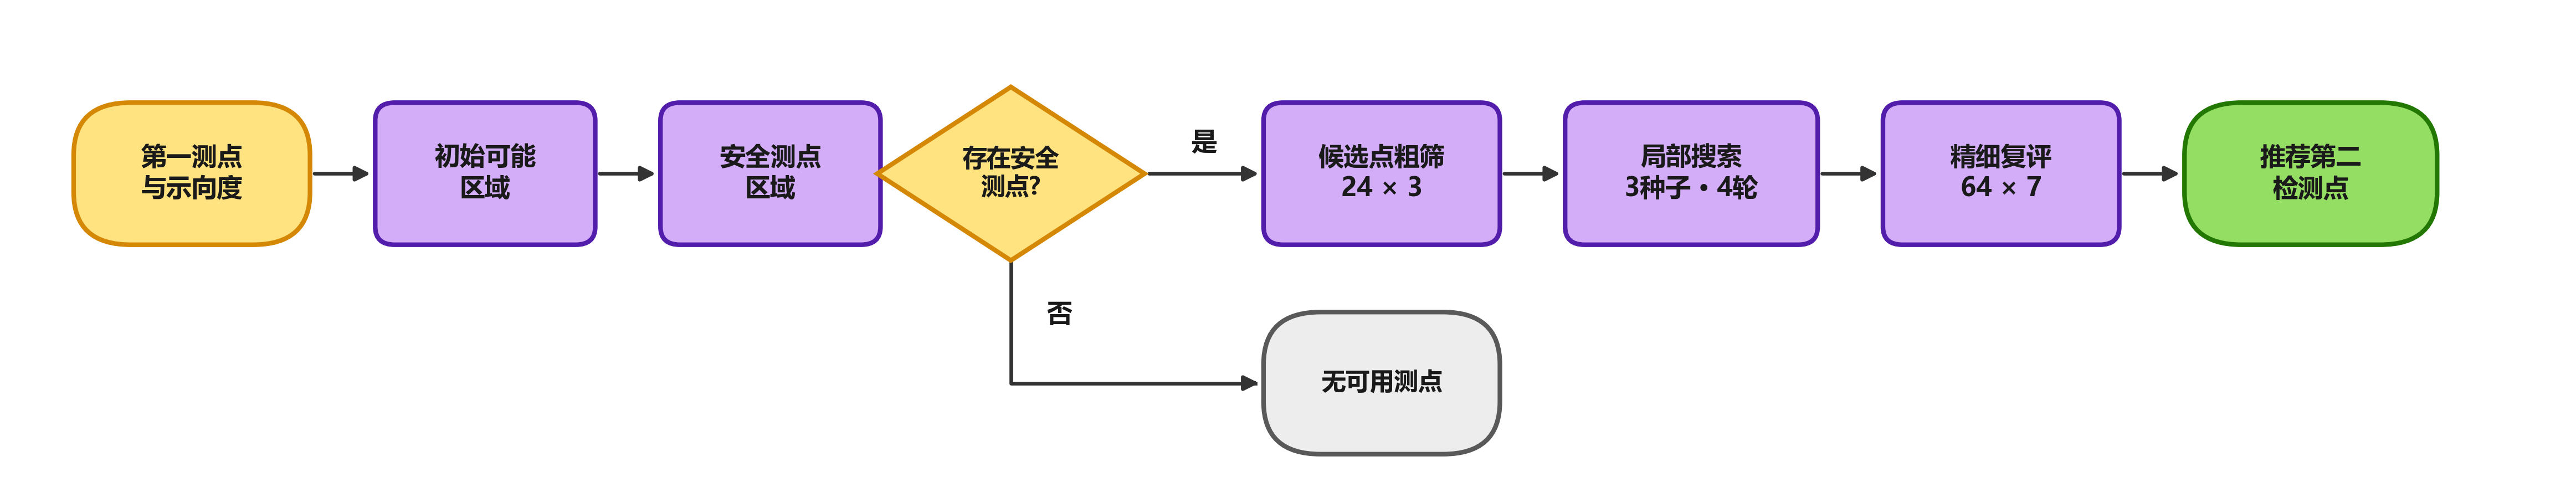
\includegraphics[width=0.98\linewidth]{images/fig_q2_flowchart.png}
    \vspace{-0.5em}
    \caption{第二检测点三阶段快速筛选与局部搜索优化流程}
    \label{fig:q2_flowchart}
    \vspace{-0.4em}
\end{figure}

\subsection{结果分析与模型检验}

\subsubsection{基准算例与多场景验证}

记算法求得的最坏后验直径为 $\widetilde{D}_2 := \widetilde{J}_{64,7} = \widehat{J}_{64,7}(\widetilde{\mathbf{p}}_2)$，初始外包络的几何直径为 $D_1^+ = \operatorname{diam}(\mathcal{P}_1^+)$。据此，定义离散评估下的不确定性压缩比为 $\widetilde{\eta} = (D_1^+ - \widetilde{D}_2)/D_1^+$。对基准算例（$\mathbf{p}_1 = (0, 0)\text{ m}, \hat\theta_1 = 0^\circ$）进行求解，单次计算耗时约 1.2 秒，指标如表 \ref{tab:q2_results} 所示。

\begin{table}[htbp]
    \centering
    \small
    \caption{基准算例下第二检测点优化解算指标}
    \label{tab:q2_results}
    \renewcommand{\arraystretch}{1.08}
    \begin{tabularx}{\linewidth}{X c c c X}
        \toprule[1.5pt]
        \textbf{评估指标} & \textbf{符号} & \textbf{数值} & \textbf{量纲} & \textbf{说明} \\
        \midrule
        第一检测点位置 & $\mathbf{p}_1$ & $(0.00, 0.00)$ & $\text{m}$ & 初始观测位置坐标 \\
        初始实测示向度 & $\hat\theta_1$ & $0^\circ$ & 度 & 沿 $+x$ 轴正方向 \\
        推荐第二检测点 & $\widetilde{\mathbf{p}_2}$ & $(839.64, 538.75)$ & $\text{m}$ & 优化所得推荐测点坐标 \\
        机器狗移动距离 & $\|\widetilde{\mathbf{p}}_2 - \mathbf{p}_1\|_2$ & 997.62 & $\text{m}$ & 两检测点间直线机动位移 \\
        保守安全余量 & $m(\widetilde{\mathbf{p}}_2)$ & 2.38 & $\text{m}$ & 目标外包络最劣距离余量 \\
        初测外包络跨度 & $D_1^+$ & 1500.23 & $\text{m}$ & 基准算例初始外包络几何直径 \\
        离散最坏后验直径 & $\widetilde{D}_2$ & \textbf{111.90} & $\text{m}$ & 64 源点 $\times$ 7 误差节点采样复核 \\
        离散评估压缩比 & $\widetilde{\eta}$ & \textbf{92.5\%} & - & $(D_1^+ - \widetilde{D}_2)/D_1^+$ \\
        单例计算耗时 & $t_{\text{solve}}$ & $\sim 1.2$ & $\text{s}$ & 算法单次完整求解耗时 \\
        \bottomrule[1.5pt]
    \end{tabularx}
\end{table}

在基准算例下，初始观测可行域关于第一示向线呈轴对称分布，优化模型在理论上存在两侧对称的最优解。数值求解在示向线两侧分别获得两组镜像对称的优选测点：
\begin{equation}
    \widetilde{\mathbf{p}}_2^{(1)} = (839.64, 538.75)\text{ m}, \quad \widetilde{\mathbf{p}}_2^{(2)} = (839.64, -538.75)\text{ m}
\end{equation}
两点移动距离均为 $997.62\text{ m}$，安全余量均为 $2.38\text{ m}$。受离散采样影响，两侧测点的目标函数值存在约 $0.14\text{ m}$ 的数值微差（正侧 $111.90\text{ m}$，负侧 $112.04\text{ m}$）。选取正侧测点作为推荐结果，其最坏后验直径由初测的 $1500.23\text{ m}$ 降至 $111.90\text{ m}$，不确定性压缩比达到 $92.5\%$。

\begin{figure}[htbp]
    \centering
    \vspace{0.2em}
    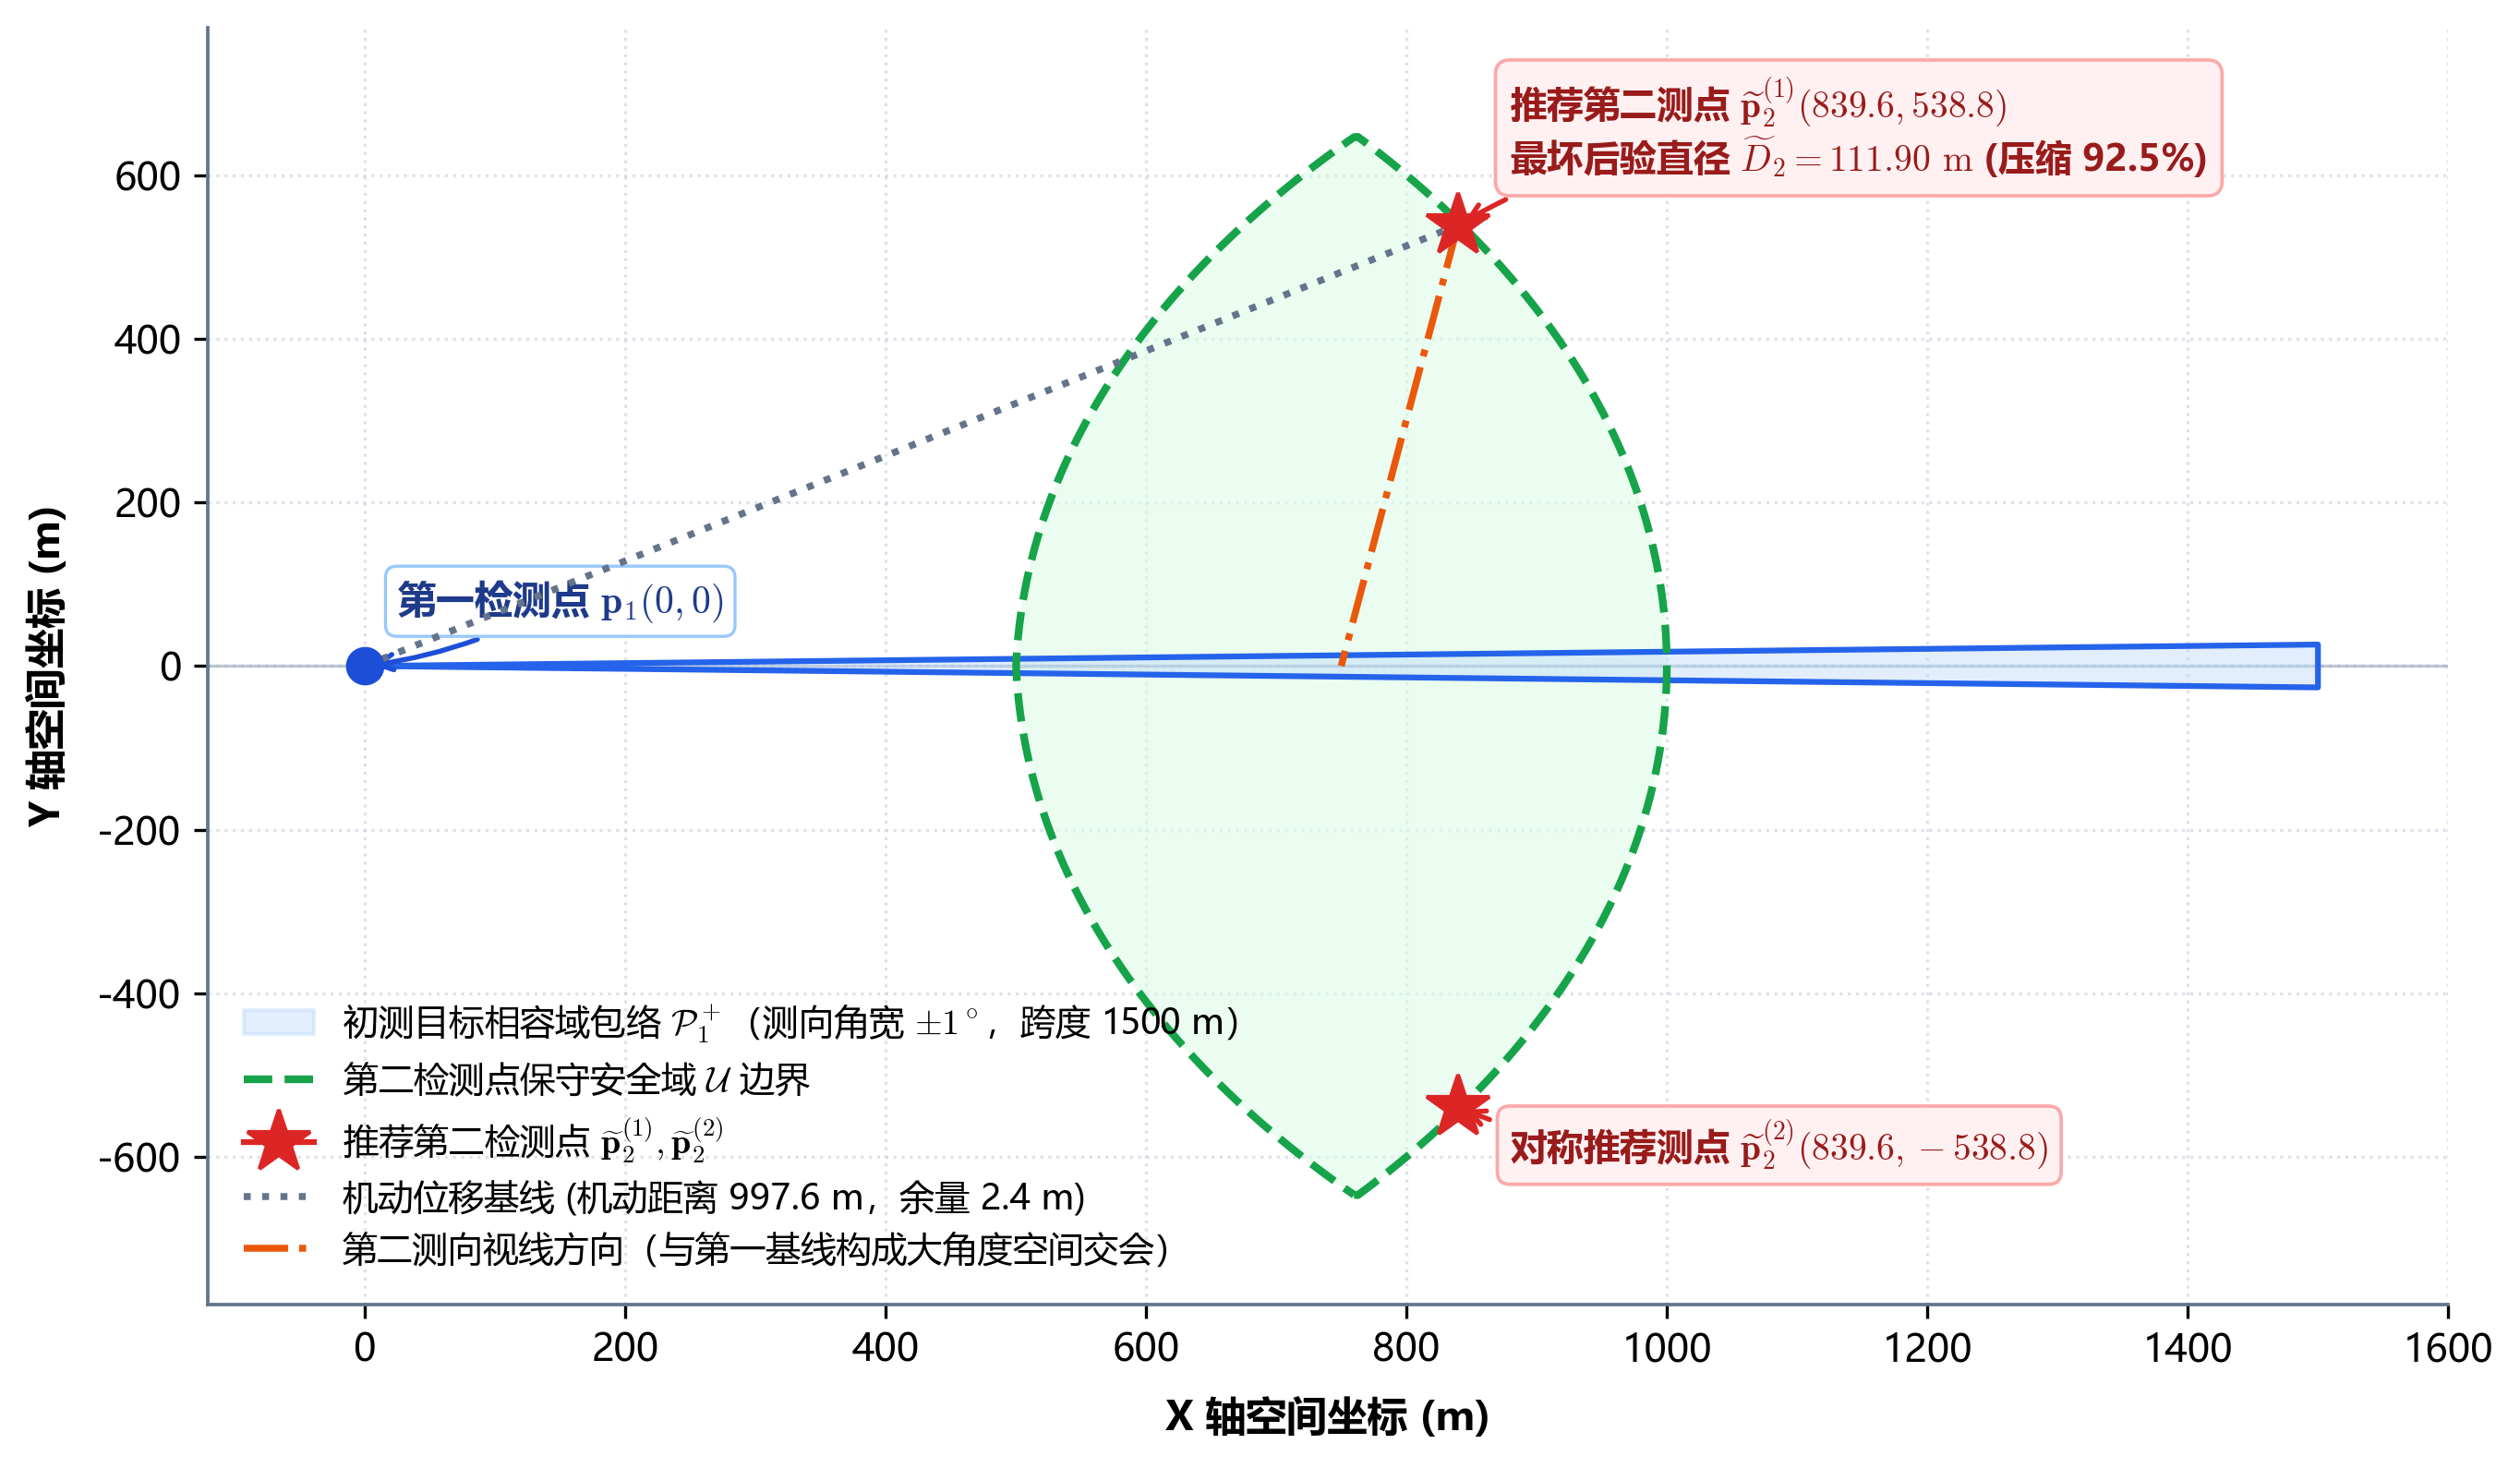
\includegraphics[width=0.76\linewidth]{images/fig_q2_candidate_region.png}
    \vspace{-0.5em}
    \caption{第二检测点保守安全域 $\mathcal{U}$ 与推荐测点几何分布图}
    \label{fig:q2_candidate_region}
    \vspace{-0.4em}
\end{figure}

图 \ref{fig:q2_candidate_region} 展示了保守安全域 $\mathcal{U}$ 的几何形态及推荐测点分布。从几何机理来看，推荐测点分布于第一示向线两侧，其核心优势在于拉大空间交会角，有效避免小角度交会造成的后验多边形径向过度拉伸 \cite{dogancay2008}，并在机动距离与定位精度间实现综合折中 \cite{vanderhook2014}；更为关键的是，该构型并非人为机械预设固定的正交夹角，而是由最差后验几何直径指标内生驱动得出的最优决策。

为进一步检验算法对不同几何构型的适应性，对圆心、偏置、切向及圆外等 6 个代表性测试场景开展求解，结果如表 \ref{tab:q2_scenarios} 所示。

\begin{table}[htbp]
    \centering
    \footnotesize
    \vspace{-0.6em}
    \caption{快速模型在不同测试场景下的实际解算结果对比}
    \label{tab:q2_scenarios}
    \renewcommand{\arraystretch}{1.04}
    \begin{tabularx}{\linewidth}{l c c c c c c X}
        \toprule[1.5pt]
        \textbf{测试场景} & \textbf{第一测点与示向} & \textbf{推荐测点} $\widetilde{\mathbf{p}}_2$ & \textbf{余量} & $D_1^+$ & $\widetilde{D}_2$ & \textbf{压缩比} & \textbf{耗时与场景说明} \\
        \midrule
        中心基准 & $(0, 0)\text{ m},\; 0^\circ$ & $(839.6, 538.8)\text{ m}$ & $2.38\text{ m}$ & $1500.2\text{ m}$ & $111.90\text{ m}$ & $92.5\%$ & $1.20\text{ s}$，对称交会 \\
        偏置场景 & $(300, 500)\text{ m},\; 125^\circ$ & $(-615.9, 898.5)\text{ m}$ & $1.16\text{ m}$ & $1493.9\text{ m}$ & $107.21\text{ m}$ & $92.8\%$ & $1.18\text{ s}$，内部非对称 \\
        边缘内指 & $(1600, 0)\text{ m},\; 180^\circ$ & $(760.4, -538.8)\text{ m}$ & $2.38\text{ m}$ & $1500.2\text{ m}$ & $111.90\text{ m}$ & $92.5\%$ & $1.22\text{ s}$，边界指心 \\
        边缘切向 & $(1600, 0)\text{ m},\; 90^\circ$ & $(1021.8, 605.0)\text{ m}$ & $163.20\text{ m}$ & $854.7\text{ m}$ & \textbf{41.41 m} & \textbf{95.2\%} & $1.28\text{ s}$，目标圆截断 \\
        圆外内指 & $(2000, 0)\text{ m},\; 180^\circ$ & $(911.1, 454.0)\text{ m}$ & \textbf{0.27 m} & $1300.3\text{ m}$ & $85.87\text{ m}$ & $93.4\%$ & $1.30\text{ s}$，圆外测点余量极敏感 \\
        跨界回绕 & $(0, 0)\text{ m},\; 359.5^\circ$ & $(844.6, 531.3)\text{ m}$ & $2.20\text{ m}$ & $1500.5\text{ m}$ & $111.87\text{ m}$ & $92.5\%$ & $1.24\text{ s}$，角度平滑跨越 \\
        \bottomrule[1.5pt]
    \end{tabularx}
    \vspace{-0.6em}
\end{table}

在基准测试中，六个代表性场景单次解算耗时均在 $1.18\sim 1.30\text{ s}$ 之间，后验定位直径较初测外包络显著压缩，展现出良好的模型稳健性与实时求解性能。特别地，在圆外场景中无缓冲推荐测点的安全余量仅为 $0.27\text{ m}$，表明在纯定位精度导向下最优测点易贴近安全域边界，实际工程应用中宜结合平台控制精度设置物理安全缓冲。

\subsubsection{近优候选区域}

为给出具体的较优候选区域，在基准算例下以网格步长 $h=25\text{ m}$ 对保守安全域 $\mathcal{U}$ 实施全域网格扫描。扫描范围由各安全圆盘的公共包围盒确定，即 $x\in[500, 1000]\text{ m}$、$y\in[-950, 950]\text{ m}$，其中共有 702 个有效安全网格点。对这些网格点，采用与全域粗筛阶段一致的 24 个代表源点和 3 个误差节点计算离散指标 $\widehat{J}_{24,3}$。全域网格最优值为 $111.893\text{ m}$，对应最优网格点 $(850, 525)\text{ m}$。各近优候选区域计算结果汇总于表 \ref{tab:q2_near_optimal}，其中区域面积按入选网格点数乘以单个网格单元面积（$h^2=625\text{ m}^2$）进行估算。

\begin{table}[htbp]
    \centering
    \small
    \vspace{-0.3em}
    \caption{基准算例下不同容差近优候选域 $\widehat{\mathcal{C}}_{\tau, h}$ 的 $25\text{ m}$ 网格统计}
    \label{tab:q2_near_optimal}
    \renewcommand{\arraystretch}{1.05}
    \begin{tabularx}{\linewidth}{c c c c c >{\raggedright\arraybackslash}X}
        \toprule[1.5pt]
        \textbf{相对容差} $\tau$ & \textbf{直径阈值} & \textbf{网格点数} & \textbf{网格面积估计} & \textbf{8-连通分量} & \textbf{总包围盒} $(x, y)$ \\
        \midrule
        $1\%$ & $113.012\text{ m}$ & 4 & $0.0025\text{ km}^2$ & 4 & $[800, 850]\times[-600, 600]\text{ m}$ \\
        $3\%$ & $115.250\text{ m}$ & 14 & $0.00875\text{ km}^2$ & 2 & $[775, 875]\times[-625, 625]\text{ m}$ \\
        $5\%$ & $117.488\text{ m}$ & 28 & $0.0175\text{ km}^2$ & 2 & $[750, 900]\times[-625, 625]\text{ m}$ \\
        \bottomrule[1.5pt]
    \end{tabularx}
    \vspace{-0.4em}
\end{table}

计算结果表明：当相对容差 $\tau$ 取 $3\%$ 与 $5\%$ 时，近优候选区域在初始示向线两侧各形成一个连通分支，呈现严格的对称分布；当容差收紧至 $1\%$ 时，候选区域高度集中于最优测点邻域，在 $25\text{ m}$ 网格步长下包含 4 个相邻网格点。

\begin{figure}[htbp]
    \centering
    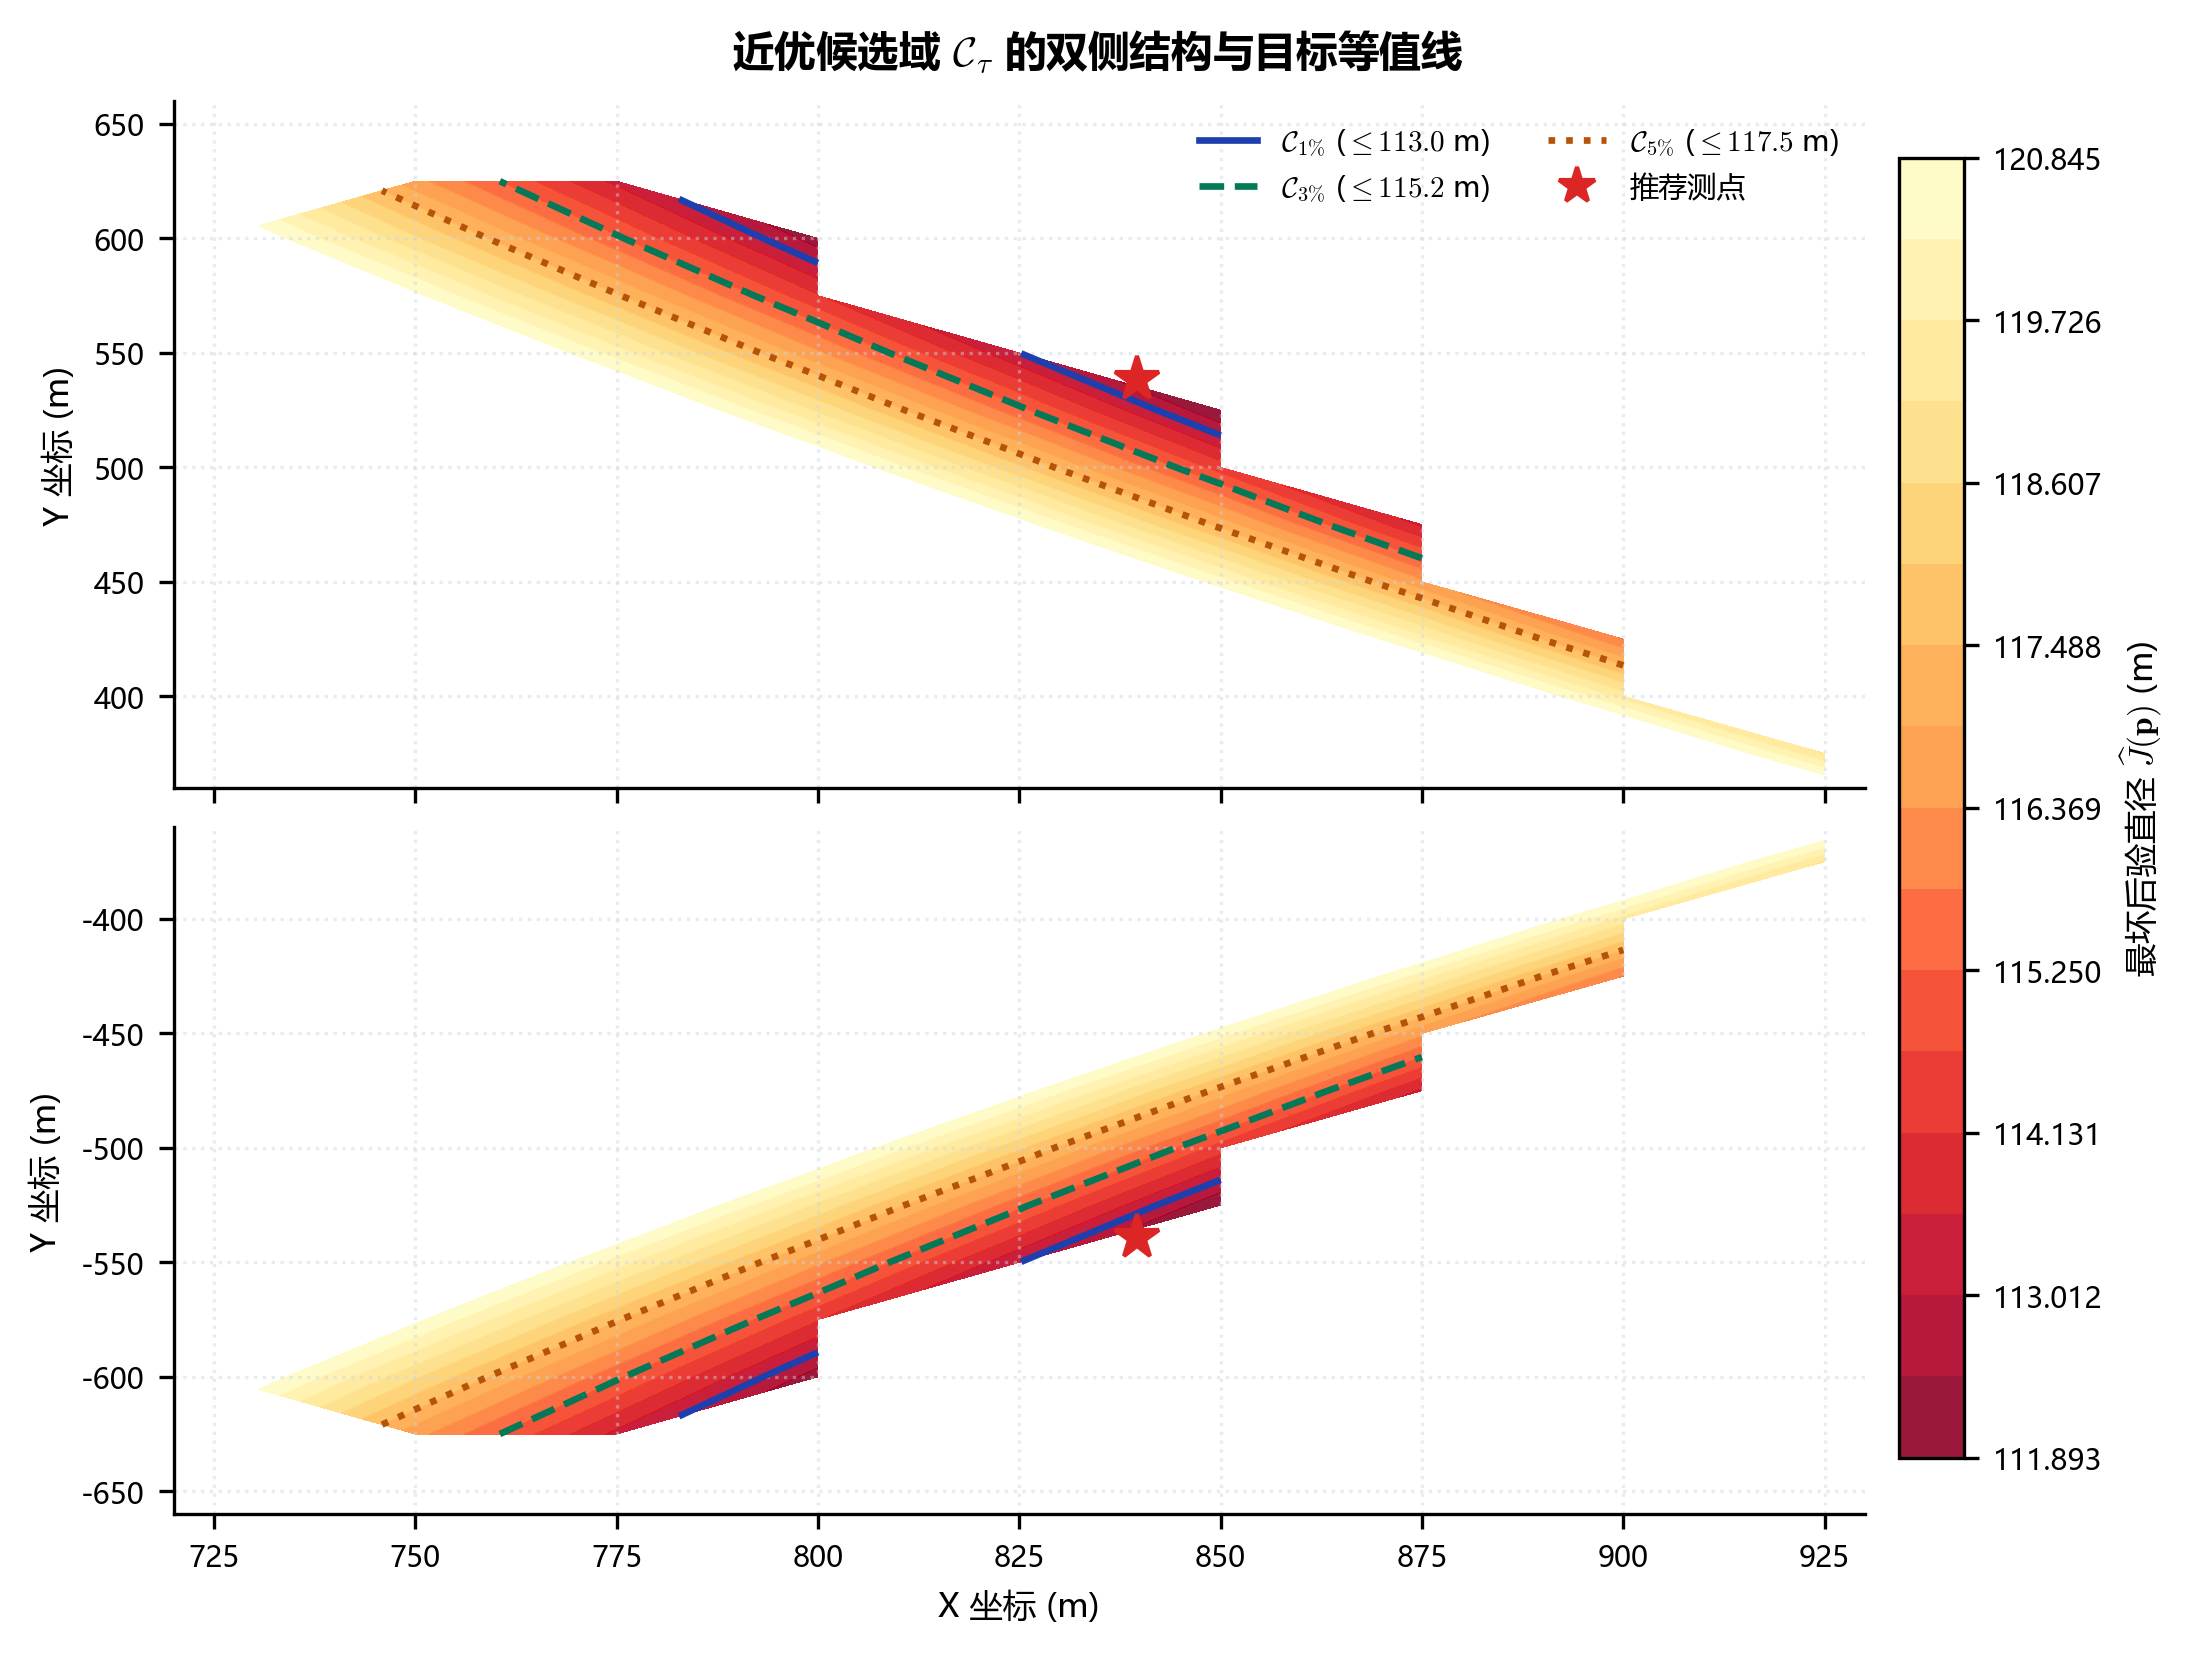
\includegraphics[width=0.78\linewidth]{images/fig_q2_candidate_contour.png}
    \vspace{-0.5em}
    \caption{基准算例下近优候选域 $\mathcal{C}_{\tau}$ 的双侧结构与最坏后验直径等值线分布图}
    \label{fig:q2_candidate_contour}
    \vspace{-0.5em}
\end{figure}

\subsubsection{运行稳定性检验}

为排除单次计算的偶然波动，对表 \ref{tab:q2_scenarios} 中的 6 个代表性场景分别独立重复执行 20 次完整解算（共计 120 次）。表 \ref{tab:q2_runtime_stats} 给出了各场景耗时的统计均值、标准差、中位数、95 分位数（P95）及最大值。

\begin{table}[htbp]
    \centering
    \small
    \caption{六大测试场景各 20 次独立完整解算耗时统计表（单位：$\text{s}$）}
    \label{tab:q2_runtime_stats}
    \renewcommand{\arraystretch}{1.06}
    \begin{tabular*}{\linewidth}{@{\extracolsep{\fill}}l c c c c c}
        \toprule[1.5pt]
        \textbf{测试场景} & \textbf{耗时均值} & \textbf{标准差} & \textbf{中位数} & \textbf{P95 分位数} & \textbf{最大耗时} \\
        \midrule
        中心基准 & 1.224 & 0.019 & 1.223 & 1.253 & 1.270 \\
        偏置场景 & 1.216 & 0.012 & 1.214 & 1.232 & 1.250 \\
        边缘内指 & 1.238 & 0.016 & 1.234 & 1.273 & 1.275 \\
        边缘切向 & 1.286 & 0.017 & 1.284 & 1.313 & 1.326 \\
        圆外内指 & 1.264 & 0.009 & 1.264 & 1.282 & 1.286 \\
        跨界回绕 & 1.268 & 0.010 & 1.265 & 1.286 & 1.292 \\
        \bottomrule[1.5pt]
    \end{tabular*}
\end{table}

实测表明，各场景平均耗时稳定在 $1.216\sim 1.286\text{ s}$，P95 均不超过 $1.313\text{ s}$，全样本最大耗时仅 $1.326\text{ s}$，且变异系数均低于 $2\%$。统计结果证实该算法计算效率高度稳定，完全能够支持机器狗在动态任务中进行实时在线决策。

\subsubsection{安全缓冲敏感性分析}

将信号接收安全要求由 $m(\mathbf{p}_2)\ge 0$ 收紧为带有物理安全缓冲 $b > 0$ 的约束 $m(\mathbf{p}_2) \ge b$。在算法实现中，仅将选点安全约束半径收紧为 $R_{\min}-b$，而发射源的初始后验状态集 $\mathcal{P}_1^+$ 仍基于真实通信距离 $R_{\min}=1000\text{ m}$ 构建，避免因人为引入安全缓冲而错误缩小目标可行域。中心基准场景下的敏感性解算结果汇总于表 \ref{tab:q2_safety_buffer}。

\begin{table}[htbp]
    \centering
    \small
    \caption{中心基准场景下不同安全缓冲距离 $b$ 的选点敏感性分析表}
    \label{tab:q2_safety_buffer}
    \renewcommand{\arraystretch}{1.06}
    \begin{tabular*}{\linewidth}{@{\extracolsep{\fill}}c c c c c}
        \toprule[1.5pt]
        \textbf{安全缓冲} $b$ & \textbf{推荐测点坐标} $(x, y)$ & \textbf{实际安全余量} $m$ & \textbf{最坏后验直径} $\widetilde{D}_2$ & \textbf{相对} $b=0$ \textbf{性能损失} \\
        \midrule
        $0\text{ m}$ & $(839.6, 538.8)\text{ m}$ & $2.38\text{ m}$ & $111.90\text{ m}$ & 基准 ($0\%$) \\
        $5\text{ m}$ & $(837.9, 532.6)\text{ m}$ & $7.20\text{ m}$ & $112.85\text{ m}$ & $+0.85\%$ \\
        $10\text{ m}$ & $(836.1, 526.4)\text{ m}$ & $12.03\text{ m}$ & $113.47\text{ m}$ & $+1.40\%$ \\
        $20\text{ m}$ & $(832.5, 513.8)\text{ m}$ & $21.71\text{ m}$ & $115.37\text{ m}$ & $+3.11\%$ \\
        \bottomrule[1.5pt]
    \end{tabular*}
\end{table}

由表 \ref{tab:q2_safety_buffer} 可知，当预留 $10\text{ m}$ 的安全缓冲时，推荐测点向安全域内部适当收缩，实际安全余量提升至 $12.03\text{ m}$，而后验直径仅增加 $1.57\text{ m}$（相对性能损失仅 $1.40\%$），表明系统在牺牲极小定位精度的前提下可显著提升行进安全性。

进一步地，设 $r_{\mathrm{MEC}}$ 为外包络 $\mathcal{P}_1^+$ 的最小外接圆半径，则安全圆盘交集非空的理论充要条件为：
\begin{equation}
    b \le b_{\max} = R_{\min} - r_{\mathrm{MEC}}
\end{equation}
对于圆外内指场景，外包络最小外接圆半径为 $r_{\mathrm{MEC}} = 650.268\text{ m}$，该场景理论最大容许缓冲为 $b_{\max} = 349.732\text{ m}$。数值扫描验证表明：在 $b=349\text{ m}$ 时算法仍能解出可行测点（$\widetilde{D}_2 = 650.27\text{ m}$），而在 $b=350\text{ m}$ 时安全域为空集，算法返回无解标识，与理论极限吻合。在 $b=0$ 时，由于模型以极小化后验直径为主目标，优选测点贴近安全域边界，安全余量仅为 $0.27\text{ m}$。设置物理安全缓冲 $b>0$ 后，候选区域向最小外接圆圆心收缩，算法也通过自适应后撤推荐测点，以满足新的缓冲要求。与此同时，最坏后验直径平缓增大，反映了信号接收安全性与定位精度之间的权衡。本节建立的选点优化模型与安全域分析方法，为后续多阶段搜索与机动决策提供了计算基础。

\section{问题三：全向干扰源的搜索定位与清除}

\subsection{问题分析}

问题三要求机器狗在半径 $R_{\mathrm{target}} = 1800\text{ m}$ 的圆形区域内，自主搜索、定位并清除全部未知的全向干扰源，在确保无一遗漏的前提下极小化任务总时间。相比前两问，该任务面临三重更为严苛的物理约束与现实挑战：
\begin{enumerate}[leftmargin=2.5em, itemsep=0.15em]
    \item \textbf{先验信息完全未知}：真实目标数量 $N \in [10, 16]$、所属频段 $\mathcal{C} = \{1, \dots, 20\}$、空间物理坐标 $\mathbf{s}_c$ 及各频道的有效接收半径 $R_c \in [1000, 1500]\text{ m}$ 事先均未知；
    \item \textbf{空间观测存在区域异构性}：机载测向传感器存在确界误差 $[-1^\circ, 1^\circ]$；当机器狗与目标间距 $\le 5\text{ m}$ 时，由于信号饱和无法测向，但可直接实施有效清除；$5\sim 20\text{ m}$ 区间内兼具测向与清除条件；$20\text{ m}\sim R_c$ 仅具备测向条件；超出 $R_c$ 则无任何信号响应；
    \item \textbf{无外部终止提示}：外部环境不主动提供剩余存活目标数或任务完成信号，系统必须完全依赖机载记录与状态空间演化，自主确证全场目标已彻底清除并安全决断终止。
\end{enumerate}

为确保全场所有客观存在的干扰源被彻底清除，首要目标为清除率达到 100\%，在此硬性前提下极小化全任务时间，建立分层优化目标：
\begin{equation}
    \operatorname{lex}\min \left\{ 1 - \eta_{\mathrm{clear}},\; T_{\mathrm{total}} \right\}
\end{equation}
其中 $\eta_{\mathrm{clear}} = K/N = 1$。本文同时考虑完全清除的理论保证和在线调度效率。理论层面依次建立全域覆盖 \cite{choset2001}、真值包含、安全清除和自主退出条件，从数学上杜绝目标遗漏；执行层面则采用极小极大几何收缩准则和动态优先级调度，使多个频道能够交错完成搜索、追踪与就地清除 \cite{song2012}，从而大幅压缩行进和测向时间。

\subsection{模型建立}

\subsubsection{机器狗状态与时间模型}

机器狗在决策步 $k$ 的物理状态记为 $\mathbf{x}_k = (\mathbf{p}_k, h_k, T_k)$，分别表示当前位置、天线调谐频道与累计虚拟时间。按照模拟器的坐标指令模型，机器狗以速率 $v = 5\text{ m/s}$ 在相邻指令坐标之间直线机动，并将动作目标坐标 $\mathbf{q}$ 作为下一步的位置状态。动作集与状态转移方程为：
\begin{equation}
    a_k \in \left\{ \mathrm{measure}(\mathbf{q}, c),\; \mathrm{clear}(\mathbf{q}, c),\; \mathrm{recover},\; \mathrm{exit} \right\}
\end{equation}
\begin{equation}
    \mathbf{p}_{k+1} = \mathbf{q}, \quad
    h_{k+1} = \begin{cases} c, & a_k = \mathrm{measure}(\mathbf{q}, c) \\ h_k, & \text{其它} \end{cases}
\end{equation}
虚拟时间增量统一由位移时间、调谐时间与动作执行时间构成：
\begin{equation}
    \Delta T_k = \frac{\|\mathbf{q} - \mathbf{p}_k\|_2}{v} + \mathbb{I}(h_k \ne c \land a_k = \mathrm{measure}) \cdot 1\text{ s} + t_{\mathrm{act}}(a_k)
\end{equation}
其中动作执行时间为：测向动作 $t_{\mathrm{act}}(\mathrm{measure}) = 5\text{ s}$；清除动作 $t_{\mathrm{act}}(\mathrm{clear}) = 5\text{ s}$（3s 光学定位 + 2s 激光发射，失败则结算 3s）。

\subsubsection{观测反馈与可行域更新}

执行动作后，获得离散观测反馈 $y_k$。目标位置 $\mathbf{s}_c$ 与实际测点 $\mathbf{p}_{\mathrm{actual}}$ 满足如下几何关系：
\begin{equation}
    y_k = \begin{cases}
        \mathrm{near}, & \|\mathbf{s}_c - \mathbf{p}_{\mathrm{actual}}\|_2 \le 5\text{ m} \implies \mathbf{s}_c \in \mathcal{B}(\mathbf{p}_{\mathrm{actual}}, 5) \\
        \mathrm{direction}(\hat{\theta}), & 5\text{ m} < \|\mathbf{s}_c - \mathbf{p}_{\mathrm{actual}}\|_2 \le R_c \implies \mathbf{s}_c \in \mathcal{W}(\mathbf{p}_{\mathrm{actual}}, \hat{\theta}) \\
        \mathrm{no\_signal}, & \|\mathbf{s}_c - \mathbf{p}_{\mathrm{actual}}\|_2 > R_c \ge 1000\text{ m} \implies \mathbf{s}_c \notin \mathcal{B}(\mathbf{p}_{\mathrm{actual}}, 1000) \\
        \mathrm{clear\_success}, & \|\mathbf{s}_c - \mathbf{p}_{\mathrm{actual}}\|_2 \le 20\text{ m} \implies \text{清除成功} \\
        \mathrm{clear\_fail}, & \|\mathbf{s}_c - \mathbf{p}_{\mathrm{actual}}\|_2 > 20\text{ m} \implies \mathbf{s}_c \notin \mathcal{B}(\mathbf{p}_{\mathrm{actual}}, 20)
    \end{cases}
\end{equation}
其中 $\mathcal{W}(\mathbf{p}, \hat{\theta})$ 为实测方位角误差半宽 $\varepsilon = 1^\circ$ 界定的双向半平面角楔。

对于每个频道 $c \in \mathcal{C}$，定义四种追踪状态：未探测 $\mathcal{S}_{\mathrm{unk}}$、探测存活 $\mathcal{S}_{\mathrm{alive}}$、已清除 $\mathcal{S}_{\mathrm{clr}}$ 与确证空置 $\mathcal{S}_{\mathrm{abs}}$。系统维护目标理论可行域 $X_{c, k}$ 的紧致凸外包多边形 $K_{c, k}^+$。频道的离散状态按照观测事件确定性转移：首次捕获角楔或近场信号后进入 $\mathcal{S}_{\mathrm{alive}}$，七个基准站均无信号时进入 $\mathcal{S}_{\mathrm{abs}}$，成功清除后进入吸收态 $\mathcal{S}_{\mathrm{clr}}$。在目标尚未清除期间，系统继续利用新获得的角楔收缩其凸外包：
\begin{equation}
    K_{c, k+1}^+ = K_{c, k}^+ \cap \mathcal{W}(\mathbf{p}_{\mathrm{actual}}, \hat{\theta})
\end{equation}
系统实时保证 $X_{c, k} \subseteq K_{c, k}^+$，只要 $K_{c, k}^+$ 满足可清除几何条件，理论可行域亦必满足，从而在保障计算凸性与数值效率的同时杜绝漏检。

\subsection{完全清除条件}

在未知目标分布、有限感知半径、测量误差以及缺乏外部终止提示的严苛条件下，单纯依赖启发式搜索无法杜绝目标遗漏风险。为此，针对全域完全清除任务建立如下数理推导与判定准则体系：
第一阶段证明七点蜂窝基准测站对目标全域的完全覆盖，确保任意位置的目标均能被探测；
第二阶段证明多次测向交会得到的凸外包多边形恒包含真实目标，确保目标物理位置不被错误剔除；
第三阶段建立基于最小外接圆与离散网格的清除判据，保证激光清除成功率并在有限步内收敛；
第四阶段给出系统自主安全退出的判定准则，确保全场无残留目标后及时退出。

\subsubsection{七点搜索网的全域覆盖}

在开展主动定位与精准清除前，首要任务是建立全域基准搜索网，确保无论未知干扰源分布在何处、有效接收半径取何值（在物理下限 $R_c \ge 1000\text{ m}$ 下），都能在有限个基准测站内被机器狗可靠探测到，从而为后续锁定与清除提供可发现性前提。

构造包含 7 个基准测站的集合 $\mathcal{Q}_7 = \{\mathbf{q}_0\} \cup \{\mathbf{q}_m\}_{m=1}^6$，其中中心站 $\mathbf{q}_0=(0,0)^\top$，外围正六边形对称站分布半径设为 $R_{\mathrm{ring}} = 1140\text{ m}$：
\begin{equation}
    \mathbf{q}_m = \left( R_{\mathrm{ring}}\cos\frac{(m-1)\pi}{3},\; R_{\mathrm{ring}}\sin\frac{(m-1)\pi}{3} \right)^\top, \quad m = 1, \dots, 6
\end{equation}

\noindent\textbf{命题 2（七点蜂窝测站实现全域无盲区覆盖）}\quad 以保守感知下限 $R_{\min} = 1000\text{ m}$ 为半径的 7 个闭圆盘之并集，严格包含半径 $1800\text{ m}$ 的目标总区域 $\mathcal{D}_0$，即 $\mathcal{D}_0 \subset \bigcup_{m=0}^6 \mathcal{B}(\mathbf{q}_m, R_{\min})$。

\begin{cumcmproof}
中心核区 $\|\mathbf{x}\|_2 \le 1000\text{ m}$ 直接落入中心基准站圆域 $\mathcal{B}(\mathbf{q}_0, 1000)$ 内。对于外环区间 $r \in [1000, 1800]\text{ m}$，考查对称主扇区 $\theta \in [0, \pi/3]$ 内点到测站 $\mathbf{q}_1$ 与 $\mathbf{q}_2$ 的欧氏距离平方 $d_1^2(r, \theta) = r^2 + R_{\mathrm{ring}}^2 - 2 r R_{\mathrm{ring}}\cos\theta$。由对称性与单调性分析，函数在角平分线 $\theta = \pi/6$ 处关于 $r$ 的偏导数为 $\frac{\partial (d_1^2)}{\partial r} = 2r - \sqrt{3}R_{\mathrm{ring}} > 0$（当 $r \ge 1000 > \frac{\sqrt{3}}{2}\times 1140 \approx 987.3\text{ m}$ 时恒正），全域距离测站最远的点位于最外周边缘处，坐标为 $\mathbf{x}_{\max} = (900\sqrt{3}, 900)^\top$。计算其与 $\mathbf{q}_1$ 的最大欧氏距离：
\begin{equation}
    d_{\max} = \|\mathbf{x}_{\max} - \mathbf{q}_1\|_2 = \sqrt{(900\sqrt{3} - 1140)^2 + 900^2} \approx 992.69\text{ m} < 1000\text{ m} = R_{\min}
\end{equation}
因全域最大距离严格小于保守感知半径，全场不存在探测盲区，目标区域全部点均被完全覆盖，命题得证。
\end{cumcmproof}

\noindent\textbf{推论}：任意客观存在的干扰源在遍历 $\mathcal{Q}_7$ 过程中必被至少一个测站探测捕获；若某一频道在 $\mathcal{Q}_7$ 全部 7 站均无信号，可严格确证该频道无目标，标记为空置 $\mathcal{S}_{\mathrm{abs}}$。七点蜂窝全域覆盖构型及机器狗执行巡航定位与激光清除的典型机动轨迹如图 \ref{fig:q3_seven_point_coverage} 所示。

\begin{figure}[htbp]
    \centering
    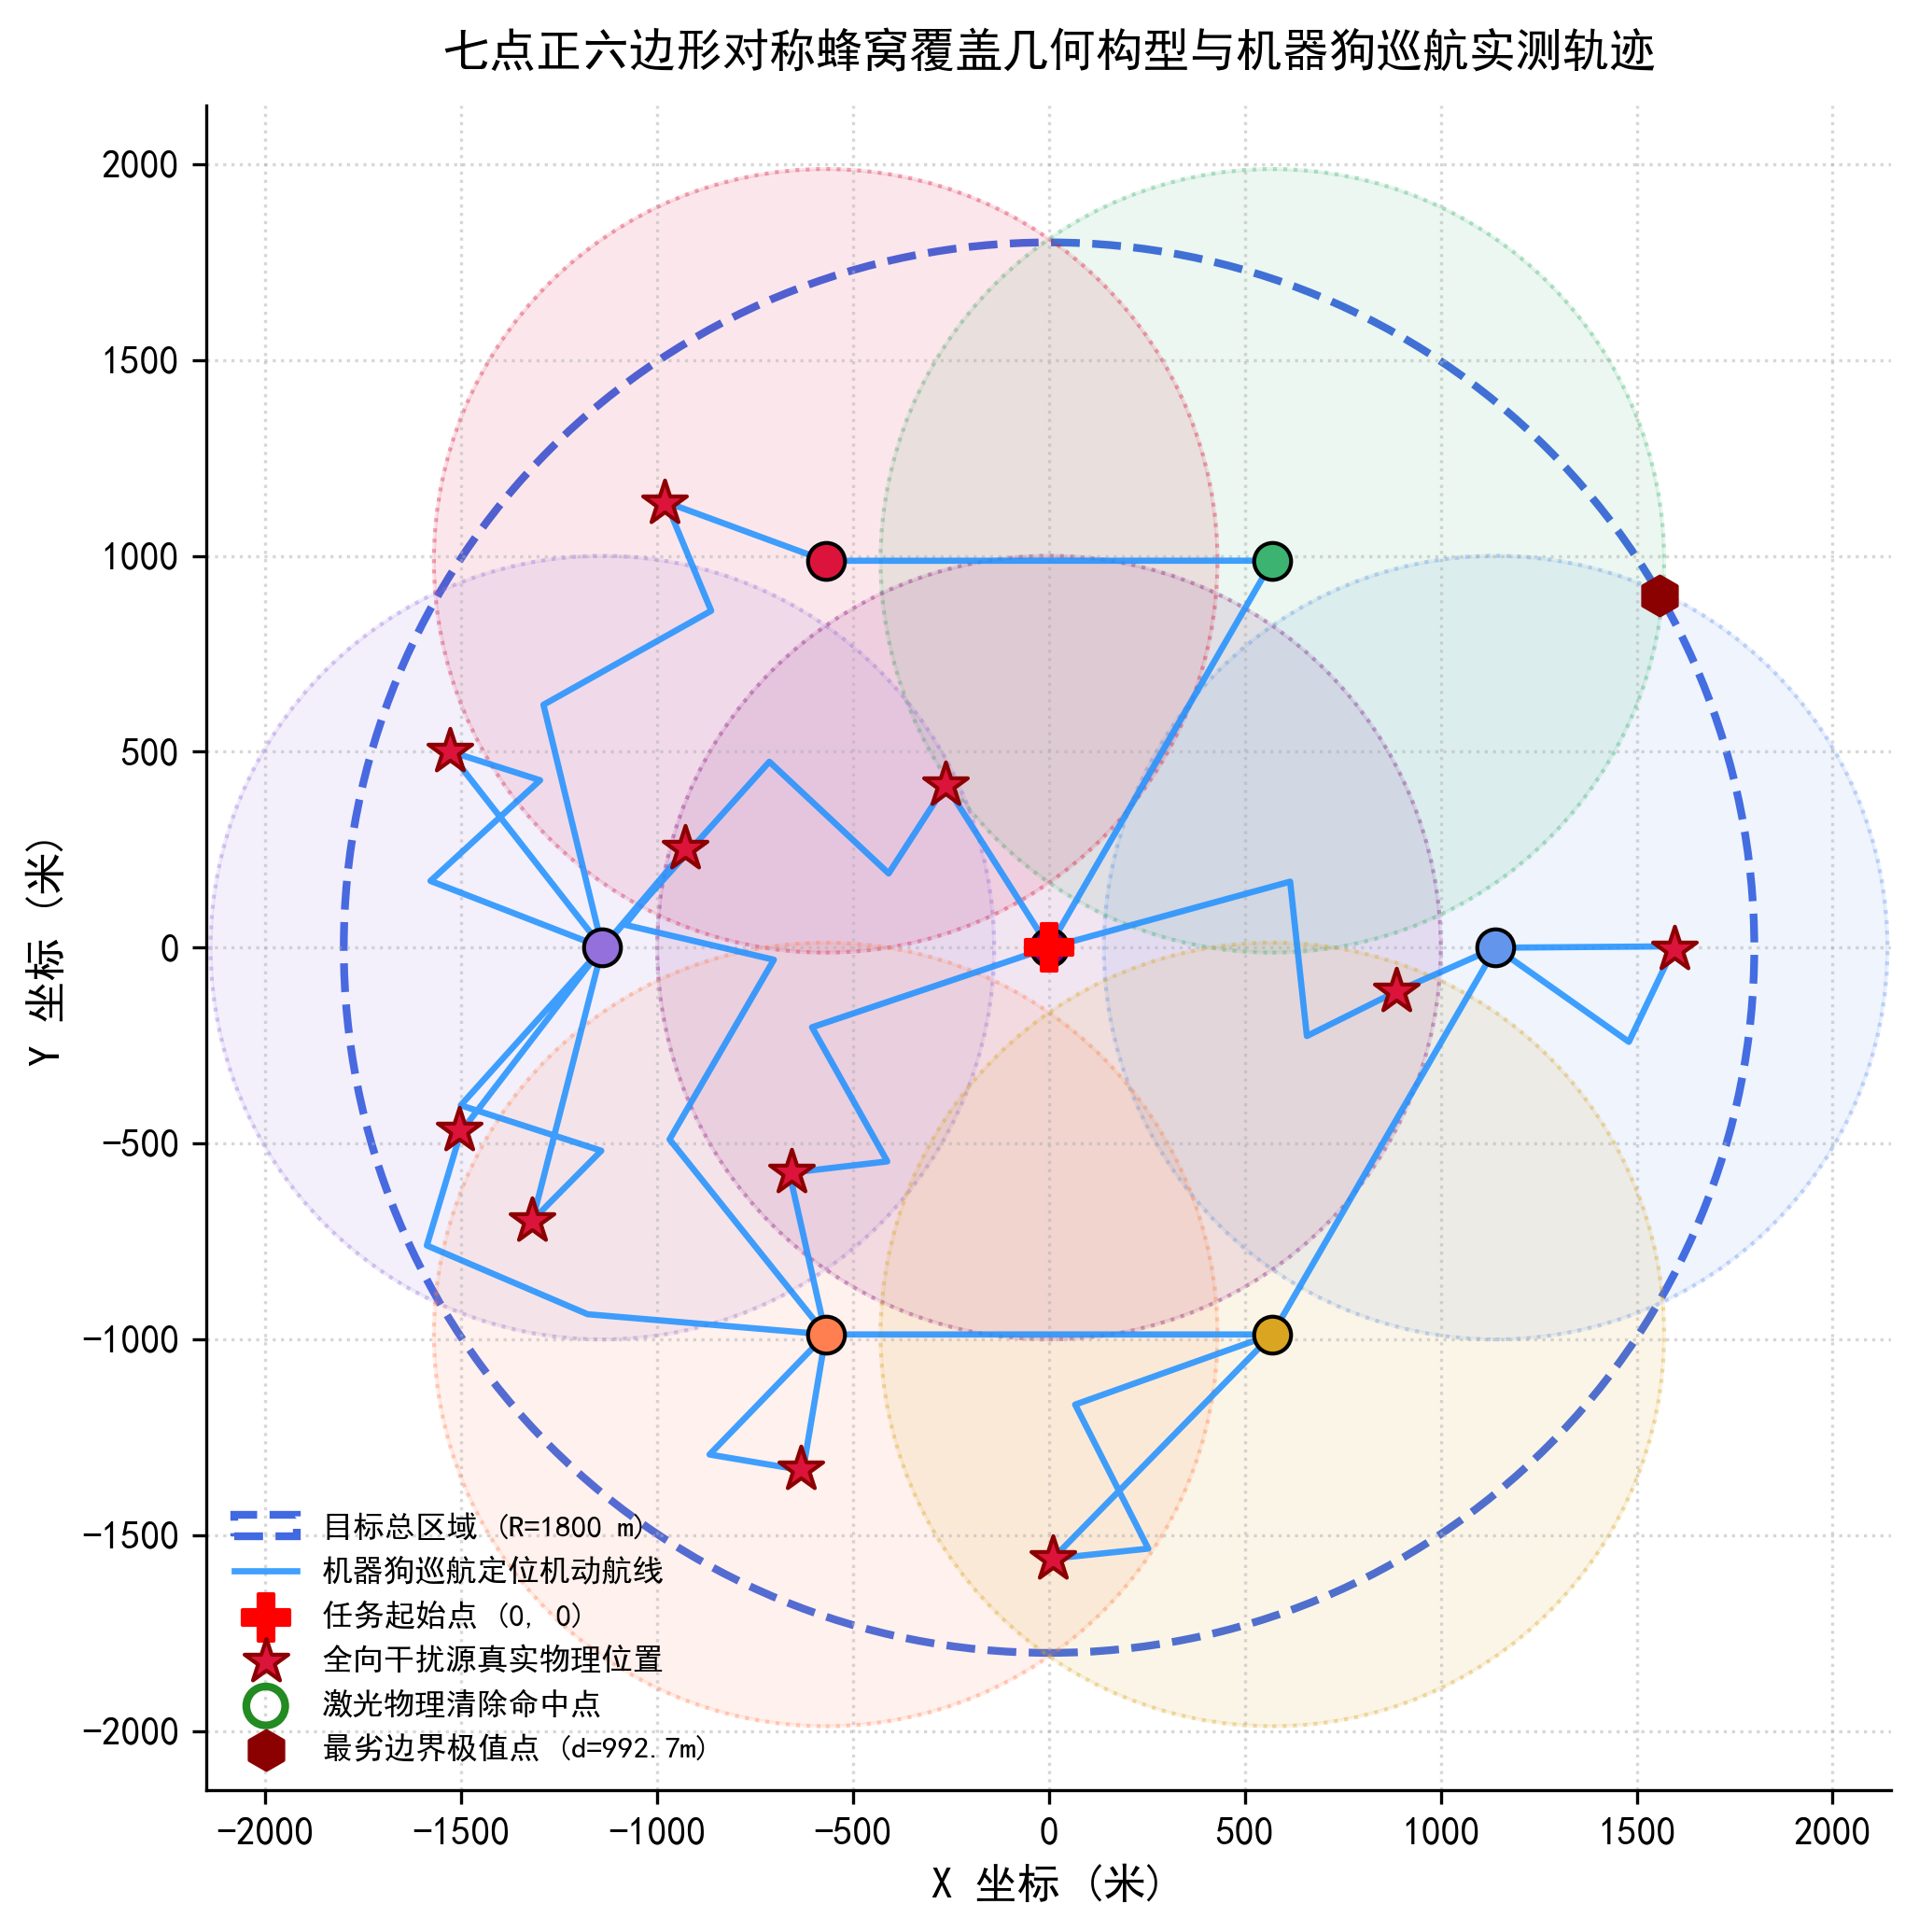
\includegraphics[width=0.96\linewidth]{images/fig_q3_seven_point_coverage.png}
    \caption{七点正六边形对称蜂窝全域覆盖几何构型(a)与机器狗巡航清除典型轨迹(b)}
    \label{fig:q3_seven_point_coverage}
\end{figure}

\subsubsection{真值包含与清除判据}

命题 2 确保了全场目标均可被可靠探测。然而，一旦某一频道首次捕获测向信号，由于机载测向仪存在确界误差 $[-1^\circ, 1^\circ]$，多次观测交汇形成的可行域必须在数学上严格保持对真实物理位置的可靠包络，避免因几何求交裁剪而将真实目标错误剔除。为此，首先确立交会凸多边形包含真实目标的数学命题。

\noindent\textbf{命题 3（交会凸多边形恒包含目标真实位置）}\quad 在任意步 $k \ge 0$，算法维护的凸外包多边形恒满足 $\mathbf{s}_c \in X_{c, k} \subseteq K_{c, k}^+$。

\begin{cumcmproof}
初始外切多边形满足 $\mathbf{s}_c \in \mathcal{P}_0$。假设第 $k$ 步包含性成立；当系统接收到新方位角 $\hat{\theta}$ 时，由测向误差界 $|\hat{\theta}-\theta^*|\le 1^\circ$ 可知，目标真值必位于对应角楔 $\mathcal{W}$ 内。因此，更新后的外包 $K_{c,k+1}^+=K_{c,k}^+\cap\mathcal{W}$ 仍包含 $\mathbf{s}_c$。若定位阶段返回 $\texttt{no\_signal}$，算法不从当前凸外包中删除区域，而是停止主动测向并进入末端直接清除判定或网格兜底，故负观测不会破坏真值包含性。由数学归纳法可知命题得证。
\end{cumcmproof}

在确立凸外包多边形 $K_{c,k}^+$ 恒包真值后，机器狗需根据外包尺度选择直接清除或网格兜底。激光清除的有效半径为 $20\text{ m}$；为降低边界浮点误差对常规定位流程的影响，本文将 $19.5\text{ m}$ 设为提前清除阈值，并保留 $20\text{ m}$ 作为主动测向预算用尽后的严格末端判定。若定位区域仍未收敛，则通过有限网格遍历完成兜底清除。记 $K_{c,k}^+$ 的最小外接圆（MEB）半径为 $r(K_{c,k}^+)$，圆心为 $\mathbf{c}(K_{c,k}^+)$。

\noindent\textbf{判据 1（最小外接圆直接清除与有限网格兜底）}\quad 针对频道 $c$ 的凸外包 $K_{c,k}^+$，采用以下分层判定：
\begin{enumerate}[leftmargin=2.5em, itemsep=0.15em]
    \item \textbf{常规定位提前清除}：若 $r(K_{c,k}^+)\le 19.5\text{ m}$，则移动至圆心 $\mathbf{c}(K_{c,k}^+)$ 实施清除。由于 $\mathbf{s}_c\in K_{c,k}^+$，有
    \begin{equation}
        \|\mathbf{s}_c-\mathbf{c}(K_{c,k}^+)\|_2\le r(K_{c,k}^+)\le 19.5\text{ m}<20\text{ m}.
    \end{equation}
    其中 $0.5\text{ m}$ 是相对于法定清除半径预留的数值稳健裕量，而非额外的物理到位误差。
    \item \textbf{测向预算结束后的直接清除}：主动测向预算用尽或无法继续生成安全候选点时，重新计算最小外接圆。若 $r(K_{c,k}^+)\le20\text{ m}$，则移动至其圆心实施清除。
    \item \textbf{有限网格兜底清除}：若仍有 $r(K_{c,k}^+)>20\text{ m}$，则将外接水平矩形剖分为边长 $\Delta g=26\text{ m}$ 的正方形网格，并遍历所有与 $K_{c,k}^+$ 相交的单元中心。每个单元中心到单元内任意点的最大距离满足
    \begin{equation}
        d_{\max}\le\frac{\sqrt{2}}{2}\Delta g\approx18.385\text{ m}<20\text{ m}.
    \end{equation}
    因此，至多经过 $M_c=\lceil W_c/\Delta g\rceil\lceil H_c/\Delta g\rceil$ 个有限网格单元即可完成兜底清除。
\end{enumerate}

\begin{figure}[htbp]
    \centering
    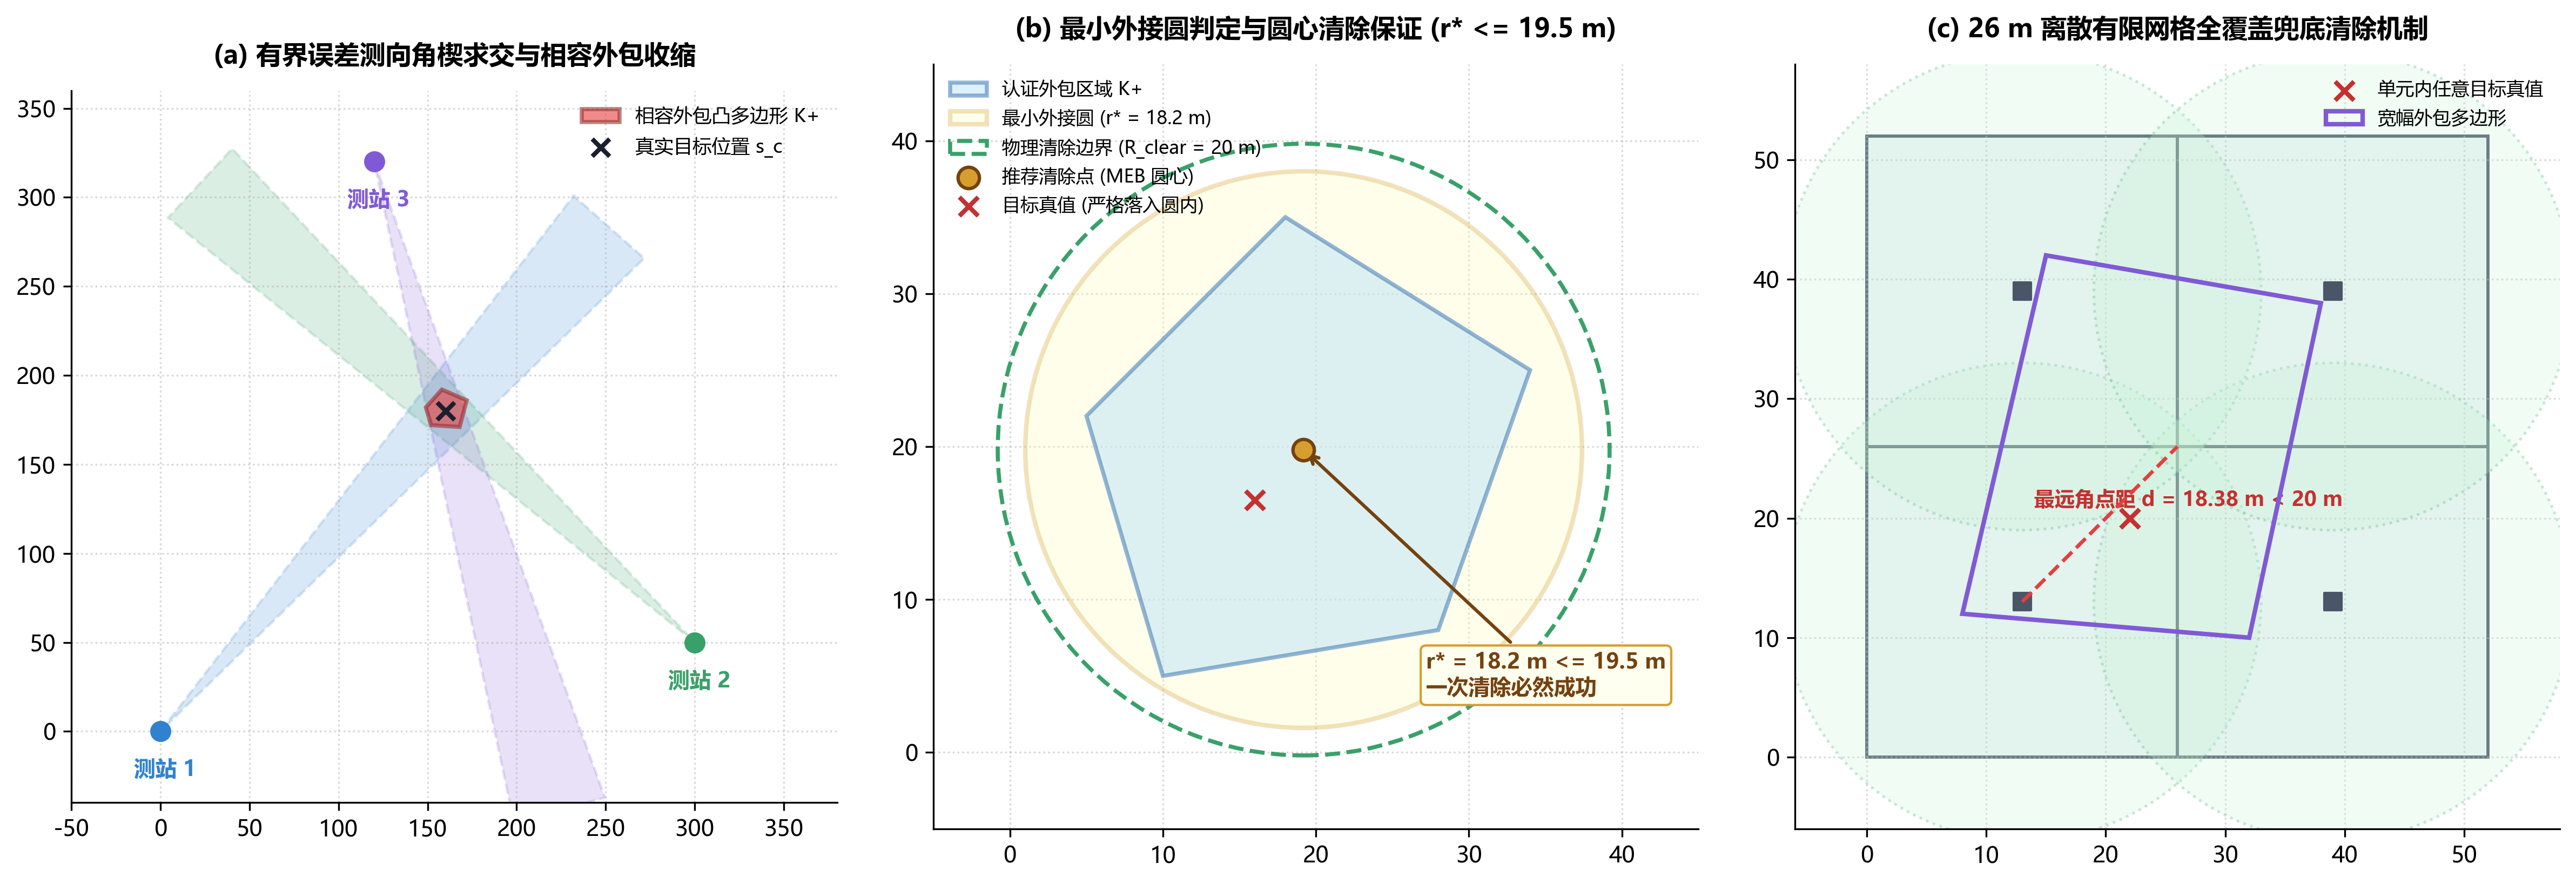
\includegraphics[width=0.86\linewidth]{images/fig_q3_geom_meb_grid.png}
    \caption{角楔交会、MEB判据与网格兜底机制示意图}
    \label{fig:q3_geom_meb_grid}
\end{figure}

\subsubsection{全局终止判定}

在完成各个被探测目标的逐一清除后，系统面临的关键决策在于：在外部环境不提供剩余存活目标总数的情况下，机器狗何时可以确信全场已绝对无任何存活目标，从而自主决断终止任务？若盲目提前退出将造成漏检，若无止境游弋则会导致时间超时。为此，依据各频道追踪状态单向转移且不回退的规律，建立全局任务自主退出的充分判定条件。记已清除频道集为 $\mathcal{C}_k^{\mathrm{cl}}$，已证实空置频道集为 $\mathcal{C}_k^{\mathrm{abs}}$。

\noindent\textbf{准则 2（全场无残留自主退出条件）}\quad 若系统无未决通信事务，且满足下列双重判定之一：
\begin{equation}
    |\mathcal{C}_k^{\mathrm{cl}}| = 16 \quad \text{或} \quad \mathcal{C}_k^{\mathrm{cl}} \cup \mathcal{C}_k^{\mathrm{abs}} = \mathcal{C}
\end{equation}
则执行退出动作 $\mathrm{exit}$ 终止任务。此时全场所有客观存在的真实干扰源已全部被清除，无一遗漏（$\eta_{\mathrm{clear}} = 1$）。

\begin{cumcmproof}
真实目标总数不超过 16，若清除 16 个目标则全场无残留；若 $\mathcal{C}_k^{\mathrm{cl}} \cup \mathcal{C}_k^{\mathrm{abs}} = \mathcal{C}$，因全体 20 频道均处于清除或已证空置的吸收态，全场无任何遗漏存活目标，清除率严格为 100\%。
\end{cumcmproof}

\subsection{定位与调度策略}

为缩短全任务时间，系统在全局层面滚动选择“继续访问未完成的七点基准站”或“处理已发现的存活频道”。一旦选中存活频道，频道内部流程再依次执行提前清除判定、主动定位、末端直接清除判定与网格兜底。该两层结构与实际程序的任务组织方式一致。

\subsubsection{安全检测点选择}
针对存活且尚未满足提前清除条件的频道，算法沿用问题二的保守候选生成与有限状态评价方法。候选点 $\mathbf b$ 必须满足
\begin{equation}
    \max_{\mathbf{x}\in K_{c,k}^+}\|\mathbf b-\mathbf x\|_2\le995\text{ m},
\end{equation}
从而在最小接收半径为 $1000\text{ m}$ 时仍保留 $5\text{ m}$ 的数值安全余量。记 $\widehat D_c(\mathbf b)$ 为 30 个代表目标位置与 3 个误差节点下得到的离散最坏后验直径，$\mathbf c_c$ 为当前外包的最小外接圆圆心，并定义
\begin{equation}
    L_c(\mathbf b)=\|\mathbf p_k-\mathbf b\|_2+\|\mathbf b-\mathbf c_c\|_2,
    \qquad
    E_c(\mathbf b)=\max\{0,\widehat D_c(\mathbf b)-39\text{ m}\}.
\end{equation}
算法按照下列四元组作字典序最小化：
\begin{equation}
    \left(
    L_c(\mathbf b)+0.85E_c(\mathbf b),\;
    \widehat D_c(\mathbf b),\;
    L_c(\mathbf b),\;
    -m_c(\mathbf b)
    \right),
\end{equation}
其中 $m_c(\mathbf b)=995\text{ m}-\max_{\mathbf{x}\in K_{c,k}^+}\|\mathbf b-\mathbf x\|_2$ 为保守接收余量。离散粗筛后，算法选取排序最优的 3 个候选作为种子，分别进行 3 轮八方向局部精修。该评价同时考虑测量后前往当前目标中心的机动距离和超出 $39\text{ m}$ 目标直径的后验不确定性。

\subsubsection{滚动任务调度}
在全局层面，记未访问基准站任务与存活频道任务的并集为 $\mathcal T_k=\mathcal T_k^{\mathrm{search}}\cup\mathcal T_k^{\mathrm{source}}$。对任务 $\tau$ 定义目标位置 $\mathbf q_\tau$、类别优先级 $\pi_\tau$ 与稳定索引 $i_\tau$，其中存活频道取 $\pi_\tau=0$，基准站取 $\pi_\tau=1$。系统采用
\begin{equation}
    \tau_k=\arg\min_{\tau\in\mathcal T_k}
    \left(\|\mathbf p_k-\mathbf q_\tau\|_2,\;\pi_\tau,\;i_\tau\right)
\end{equation}
作字典序选择。因此，系统通常优先执行距离当前位置最近的任务；当距离相同时，先处理已发现目标，再访问基准站。清除、主动定位和网格兜底均在选中的频道内部按判据 1 顺序执行，不另设与实现不一致的固定权重评分。

\subsection{算法实现与分析}

\subsubsection{在线控制流程}

综合状态演化、完全清除条件检验与滚动调度，多全向干扰源在线搜索、定位与清除闭环状态机流程如图 \ref{fig:q3_flowchart} 所示，整体在线自主控制主算法如算法 1 所示。

\begin{figure}[htbp]
    \centering
    \vspace{0.2em}
    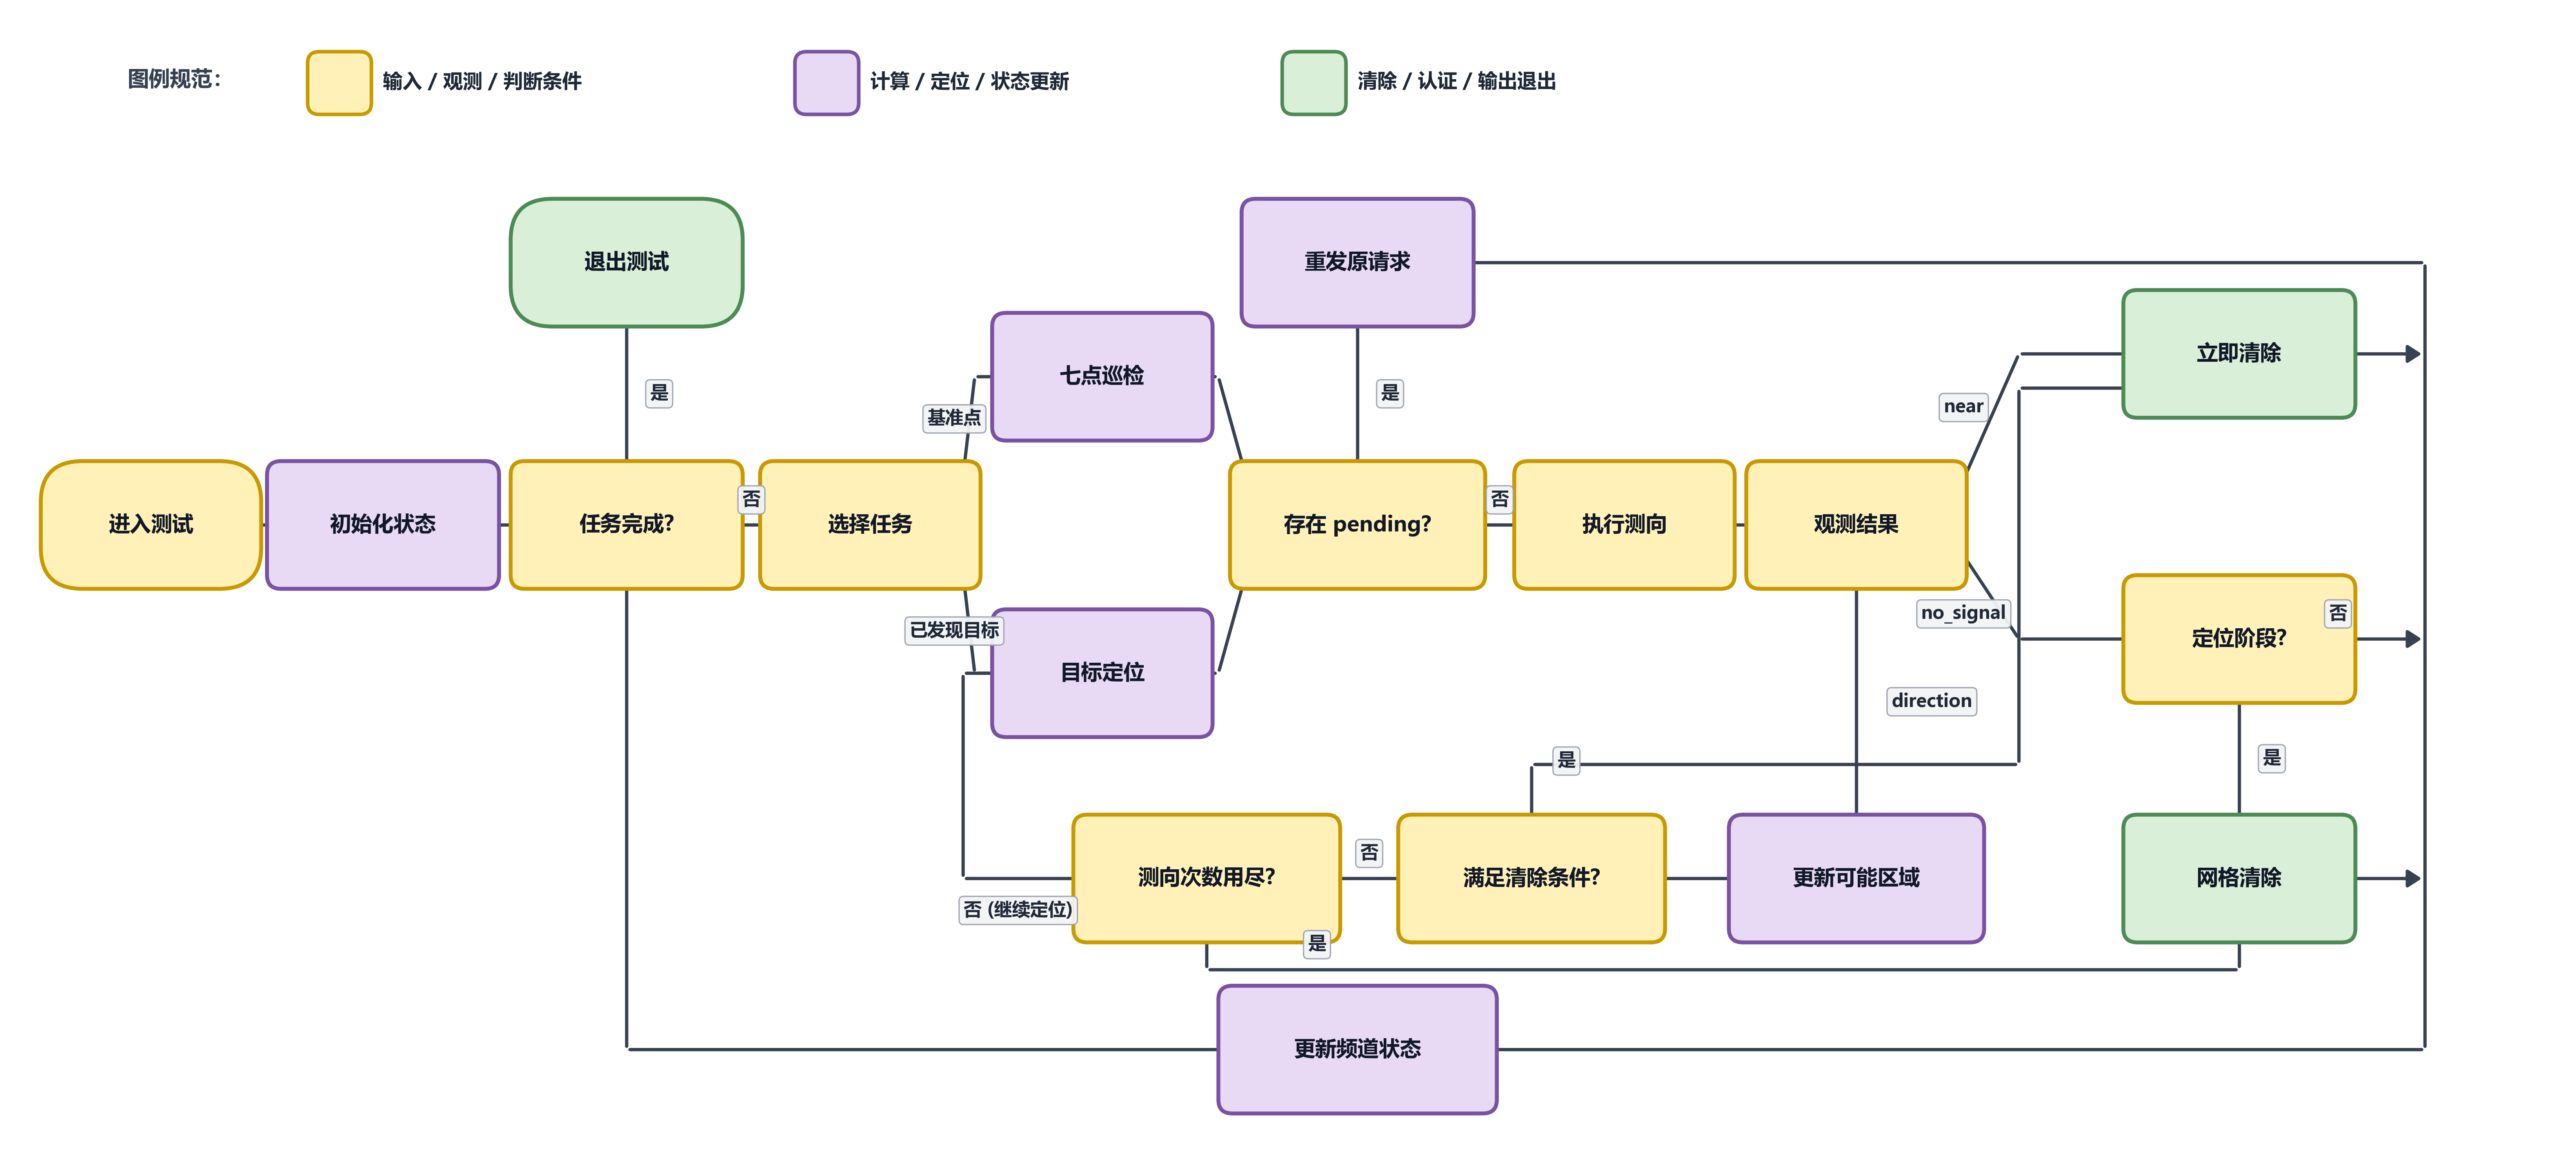
\includegraphics[width=0.96\linewidth]{images/fig_q3_flowchart.png}
    \vspace{-0.5em}
    \caption{多全向干扰源在线搜索、定位与清除闭环状态机流程}
    \label{fig:q3_flowchart}
    \vspace{-0.4em}
\end{figure}系统为每个动作请求附加唯一标识编号。若遇到未决状态（$\mathrm{pending}$），则暂停派发新任务，并使用相同载荷和相同请求编号重发原动作。程序最多重试 $N_{\mathrm{retry}}=2$ 次，即包含首次请求时单个动作最多发送 3 次；若仍无法恢复，则停止继续决策且不签发完成证书，避免把响应未知的动作误记为已完成。

\begin{table}[htbp]
    \centering
    \small
    \caption{算法 1：未知多干扰源在线协同搜索、定位与清除主算法}
    \label{alg:q3_unified_loop}
    \renewcommand{\arraystretch}{1.05}
    \begin{tabularx}{\linewidth}{l X}
        \toprule[1.5pt]
        \multicolumn{2}{X}{\textbf{输入：} 区域半径 $R_{\mathrm{target}}=1800\text{ m}$，感知下限 $R_{\min}=1000\text{ m}$，误差界 $\varepsilon=1^\circ$，频道集 $\mathcal{C}=\{1,\dots,20\}$} \\
        \multicolumn{2}{X}{\textbf{输出：} 物理动作执行序列与全场完备清除报告} \\
        \midrule
        1: & 初始化：状态 $\mathbf{p}_0=(0,0)^\top$，$h_0=1$，$T_0=0$，$\forall c \in \mathcal{C}$ 设 $L_{c,0}=\mathcal{S}_{\mathrm{unk}}$，$K_{c,0}^+=\mathcal{P}_0$，构建 $\mathcal{Q}_7$ \\
        2: & \textbf{while} 终止条件不满足 \textbf{do} \\
        3: & \quad 若存在未决事务，重新发送动作指令并跳至第 8 步； \\
        4: & \quad 检验准则 2 终止条件：若 $|\mathcal{C}_k^{\mathrm{cl}}|=16$ 或 $\mathcal{C}_k^{\mathrm{cl}} \cup \mathcal{C}_k^{\mathrm{abs}}=\mathcal{C}$，派发 $a_k = \mathrm{exit}$ 终止主循环； \\
        5: & \quad 在未访问基准站与存活频道之间，按“机动距离、任务类别、稳定索引”的字典序选择下一任务； \\
        6: & \quad 若选中存活频道，先检验 $r\le19.5\text{ m}$；否则至多进行 4 次主动测向，随后按 $r\le20\text{ m}$ 直接清除或转入 26 米网格兜底； \\
        7: & \quad 若选中基准站，则移动至该站并依次扫描尚未结案的频道；对返回的 \texttt{direction}、\texttt{near} 与 \texttt{no\_signal} 分别更新外包、就地清除或记录缺席证据； \\
        8: & \quad 将已确认的动作反馈追加至历史序列，更新物理状态、频道状态和完成证书所需证据； \\
        9: & \textbf{end while} \\
        10: & \textbf{return} 任务完备达成，输出执行动作序列与统计结果 \\
        \bottomrule[1.5pt]
    \end{tabularx}
\end{table}

\subsubsection{有限步终止性分析}

为验证算法 1 在实际调度执行中不存在死循环与死锁，下面结合七点覆盖、真值包含与退出准则，证明该搜索清除过程必在有限个离散动作步内终止：

\noindent\textbf{命题 4（搜索清除过程有限步终止）}\quad 在目标静止、测向误差满足给定确界、七点搜索网完整执行且每个已发出的通信事务均能在有限次重试内获得确定响应的条件下，算法 1 可在有限离散动作步数内完成全部实际目标的清除并安全退出。

\begin{cumcmproof}
基准搜索至多包含 $7\times20=140$ 个互不重复的检测动作，每个存活目标的主动测向次数受预算 $N_{\mathrm{loc\_max}}=4$ 限制。若目标在该预算内仍未满足直接清除条件，算法转入有限网格兜底；由于未访问单元数随清除尝试单调减少，该过程必在有限步内结束。通信事务按相同请求编号进行至多 2 次重试，并由确定响应驱动状态转移；各频道状态只会由未探明转为已发现、确证空置或已清除。因此，系统最终在有限步内满足准则 2 并退出。
\end{cumcmproof}

\noindent\textbf{计算复杂度与执行时间}：设当前凸外包的极点数为 $h$，候选点数量为 $K$，代表目标位置数量为 $S$，误差节点数量为 $E$。单个候选点的离散后验评价复杂度为 $O(SEh)$，一轮候选评价的总复杂度为 $O(KSEh)$；半平面裁剪和最小外接圆计算分别随当前极点数线性或期望线性增长。三次正式测试的程序运行时间为 $3.180\sim4.862\text{ s}$，平均为 $4.215\text{ s}$，远低于 $1200\text{ s}$ 的程序运行时限。

\subsection{测试结果与分析}

为检验当前完整策略在重复随机场景中的执行稳定性，本文使用本地模拟器对固定种子 0 至 99 的 100 个场景逐一运行。该批结果取自当前默认参数下的结构化批处理输出，种子区间与各项统计字段均保留在支撑材料中。该实验属于本地重复测试，与后文三次官方模拟器正式测试分开报告。

\subsubsection{本地重复测试}

100 个场景均完成全部目标清除，且未出现失败清除。任务时间与程序运行时间的统计结果见表 \ref{tab:q3_local_batch_results}。

\begin{table}[htbp]
    \centering
    \footnotesize
    \caption{固定种子 0 至 99 的 100 组本地重复测试结果}
    \label{tab:q3_local_batch_results}
    \renewcommand{\arraystretch}{1.0}
    \begin{tabularx}{\linewidth}{X c}
        \toprule[1.5pt]
        \textbf{统计指标} & \textbf{结果} \\
        \midrule
        完成全部目标清除的场景数 & $100/100$ \\
        全场景目标清除率 & $100\%$ \\
        虚拟任务总时间均值 & $3373.913\text{ s}$ \\
        虚拟任务总时间标准差（样本标准差） & $315.839\text{ s}$ \\
        虚拟任务总时间最大值 & $4340.883\text{ s}$ \\
        单源平均定位清除时间的场景均值 & $269.162\text{ s/源}$ \\
        程序运行时间均值 & $3.091\text{ s}$ \\
        程序运行时间最大值 & $5.239\text{ s}$ \\
        失败清除总次数 & $0$ \\
        \bottomrule[1.5pt]
    \end{tabularx}
\end{table}

该批 100 场结果表明，当前策略在所选本地场景中保持了完整清除和零失败清除。虚拟任务时间仍存在约 $315.839\text{ s}$ 的样本标准差，说明目标数量与空间分布会显著影响机动代价；因此，本批结果用于描述当前测试分布下的有限样本表现，不外推为任意分布下的总体性能。

\subsubsection{正式测试结果}

在确定关键算法参数（单目标主动测向次数上限 $N_{\mathrm{loc\_max}}=4$，提前清除阈值 $r^*=19.5\text{ m}$，末端直接清除阈值 $20\text{ m}$，网格边长 $\Delta g=26\text{ m}$）后，本文在官方模拟器中完成三次正式测试。按照题目规定的字段，测试结果汇总于表 \ref{tab:q3_official_tests}。

\begin{table}[htbp]
    \centering
    \footnotesize
    \caption{基于赛题规范模拟环境的三次测试结果汇总表}
    \label{tab:q3_official_tests}
    \renewcommand{\arraystretch}{1.0}
    \setlength{\tabcolsep}{3.5pt}
    \begin{tabular*}{\linewidth}{@{\extracolsep{\fill}}l c c c}
        \toprule[1.5pt]
        \textbf{正式测试案例编码} & \textbf{清除数量} & \textbf{平均定位清除时间/s} & \textbf{程序运行时间/s} \\
        \midrule
        \texttt{2T4W-AQ2B-BFJ9-DETS} & 11 个 & 249.178 & 3.180 \\
        \texttt{VC2X-UWRN-NBUP-2X6V} & 14 个 & 241.330 & 4.603 \\
        \texttt{M9X2-6D5X-E84D-5AEH} & 14 个 & 240.549 & 4.862 \\
        \bottomrule[1.5pt]
    \end{tabular*}
\end{table}

三次测试的虚拟任务总时间分别为 $2740.959\text{ s}$、$3378.626\text{ s}$ 与 $3367.691\text{ s}$，算术平均为 $3162.425\text{ s}$。三次测试共清除 39 个目标，按目标数量汇总后的加权平均定位清除时间为 $243.263\text{ s/源}$，程序运行时间均值为 $4.215\text{ s}$。测试结果与理论机制分析如下：
\begin{enumerate}[leftmargin=2.5em, itemsep=0.05em, topsep=0.2em]
    \item \textbf{完全清除与清除分支}：三次测试清除率均达到 100\%。39 个目标中，36 个通过外接圆圆心清除，3 个在返回 \texttt{near} 后就地清除；全部 39 次清除请求均首次执行成功，未发生失败清除；
    \item \textbf{退出条件触发规律一致}：三次测试均通过蜂窝拓扑扫描与动态状态账本，在全域 20 个频道的信号状态均确立为已清除（$\texttt{cleared}$）或已认证空置（$\texttt{absent\_certified}$）时触发准则安全退出，与理论推导吻合；
    \item \textbf{时间合规性}：最大虚拟任务时间为 $3378.626\text{ s}$，低于模拟器规定的 $360000\text{ s}$ 虚拟时间上限；程序运行时间为 $3.180\sim4.862\text{ s}$，均远低于 $1200\text{ s}$ 的程序运行上限。
\end{enumerate}


\vspace{-0.4em}
\section{问题四：混合干扰源的搜索定位与清除}
\setlength{\abovedisplayskip}{3.5pt}
\setlength{\belowdisplayskip}{3.5pt}

\subsection{问题分析}

问题四在问题三的基础上，进一步引入了半平面定向辐射干扰源。各干扰源独占单一频道的物理规律保持不变，目标总数仍处于 $10\sim 16$ 个之间。但定向干扰源的具体数目及其辐射主瓣朝向均完全未知。其余运动速度、调谐与测向耗时、测向角度误差 $[-1^\circ, 1^\circ]$、以及 $20\text{ m}$ 激光清除等条件与前述问题完全一致。

相比全向辐射，定向辐射带来了三个新的难点：
\begin{enumerate}[leftmargin=2.2em, itemsep=0.04em, topsep=0.03em]
    \item \textbf{半平面定向辐射导致无信号成因复杂}：定向源仅在其辐射朝向所确定的 $180^\circ$ 闭半平面内发射信号。测站未收到信号可能由于频道空置、目标已清除、空间超距、或测站处于发射盲侧。因此，单次无信号不能直接排除对应几何区域。
    \item \textbf{单测站无法保证发现，需多测站协同包围}：全向目标只要距离小于 $1000\text{ m}$ 即可被单测站探测；而定向目标若背对测站，即便距离很近也无法感知。要发现未知朝向的目标，必须依靠多个测站从不同方位对其形成几何包围。
    \item \textbf{追加测向耗时与网格遍历成本的平衡}：初次发现目标后，若盲目追加测向可能再次落入盲侧而徒劳失联；若完全依赖网格遍历，时间成本又过高。因此需要在基准搜索之外，建立轻量自适应决策逻辑。
\end{enumerate}

本文首先构建由 25 个测站组成的双环网络 \cite{guvensan2011}，利用凸包包围性质确保任意未知朝向的目标均能被可靠发现。在此基础上，进一步引入安全距离选点、对称镜像探测和自适应尾部探测，在确保完全清除的前提下尽量减少机动与网格遍历时间。

\subsection{模型建立}

\subsubsection{目标物理状态}

系统共有 20 个离散频道，记为 $\mathcal{C} = \{1, 2, \dots, 20\}$。对客观存在目标的频道（$e_c = 1$），其物理状态由五元组表征：
\begin{equation}
    \mathbf{X}_c = (e_c, \mathbf{x}_c, R_{c}, \tau_c, \mathbf{u}_c), \quad c \in \mathcal{C}, \; e_c = 1
\end{equation}
式中各参数含义如下：
\begin{enumerate}[leftmargin=2.2em, itemsep=0.02em, topsep=0.02em]
    \item $e_c \in \{0, 1\}$ 表示频道 $c$ 是否存在物理目标，目标总数满足 $N = \sum_{c=1}^{20} e_c \in [10, 16]$；
    \item $\mathbf{x}_c = (x_{c,1}, x_{c,2})^\top \in \Omega$ 为目标二维平面坐标；
    \item $R_{c} \in [1000, 1500]\text{ m}$ 为该目标的信号覆盖半径；
    \item $\tau_c \in \{\mathrm{O}, \mathrm{D}\}$ 表示辐射类型，$\mathrm{O}$ 为全向辐射，$\mathrm{D}$ 为半平面定向辐射；
    \item $\mathbf{u}_c = (\cos\phi_c, \sin\phi_c)^\top$ 为定向天线的法向辐射单位向量（全向目标不受该向量约束）。
\end{enumerate}
若频道无目标（$e_c = 0$），则后序分量不予定义。

为刻画作业过程中目标的清除过程，引入清除变量 $h_c^k \in \{0, 1\}$（初始为 0，清除后置为 1），定义时步 $k$ 处的动态活动变量：
\begin{equation}
    a_c^k = e_c (1 - h_c^k) \in \{0, 1\}
\end{equation}
当机器狗在目标 $20\text{ m}$ 范围内成功清除目标后，$h_c^k$ 置为 1，$a_c^k$ 变为 0。

\subsubsection{定向接收与观测模型}

对于存活目标（$a_c^k = 1$），定义其在检测位置 $\mathbf{q} = (q_1, q_2)^\top$ 处的几何可接收条件：
\begin{equation}
    \mathcal{V}_c(\mathbf{q}) = \Big[ \|\mathbf{q} - \mathbf{x}_c\| \le R_{c} \Big] \land \Big[ \tau_c = \mathrm{O} \;\lor\; \mathbf{u}_c^\top (\mathbf{q} - \mathbf{x}_c) \ge 0 \Big]
\end{equation}
包含法向分界线 $\mathbf{u}_c^\top (\mathbf{q} - \mathbf{x}_c) = 0$ 在内的平角区域均可正常通信；若测站与目标重合（$\mathbf{q} = \mathbf{x}_c$），约定处于有效视场。

为清晰厘清无信号反馈的成因，将其分解为四类互斥物理事件：
\begin{enumerate}[leftmargin=2.2em, itemsep=0.02em, topsep=0.02em]
    \item $E_0 = \{e_c = 0\}$：该频道本就未布设目标；
    \item $E_1 = \{e_c = 1, h_c^k = 1\}$：该频道目标此前已被成功清除；
    \item $E_2 = \{a_c^k = 1, \|\mathbf{q} - \mathbf{x}_c\| > R_c\}$：目标存活但距离超出接收范围；
    \item $E_3 = \{a_c^k = 1, \|\mathbf{q} - \mathbf{x}_c\| \le R_c, \tau_c = \mathrm{D}, \mathbf{u}_c^\top (\mathbf{q} - \mathbf{x}_c) < 0\}$：目标存活且在距离范围内，但测站处于定向天线的发射盲侧。
\end{enumerate}
四类事件两两互斥，其并集构成无信号事件 $E_{\mathrm{none}} = E_0 \cup E_1 \cup E_2 \cup E_3$。

测站在 $\mathbf{q}$ 处对频道 $c$ 的实测反馈 $y_c^k(\mathbf{q})$ 严格划分为三个互斥分支：
\begin{equation}
    y_c^k(\mathbf{q}) = \begin{cases}
        \texttt{no\_signal}, & E_0 \lor E_1 \lor E_2 \lor E_3, \\
        \texttt{near}, & a_c^k = 1 \;\land\; \mathcal{V}_c(\mathbf{q}) \;\land\; \|\mathbf{q} - \mathbf{x}_c\| \le 5\text{ m}, \\
        \texttt{direction}(\hat{\theta}_c), & a_c^k = 1 \;\land\; \mathcal{V}_c(\mathbf{q}) \;\land\; \|\mathbf{q} - \mathbf{x}_c\| > 5\text{ m}
    \end{cases}
\end{equation}
当返回示向角 $\hat{\theta}_c$ 时，真实方位角 $\theta_c^\ast = \operatorname{atan2}(x_{c,2} - q_2, x_{c,1} - q_1)$ 与实测示向角满足圆周角距离误差约束：
\begin{equation}
    d_{\mathbb{S}^1}(\theta_c^\ast, \hat{\theta}_c) = |\operatorname{wrap}_{[-180^\circ, 180^\circ)}(\theta_c^\ast - \hat{\theta}_c)| \le \varepsilon = 1^\circ
\end{equation}
为防止浮点截断误差在半平面求交时误删边界解，交会计算时采用容差 $\varepsilon_{\mathrm{tol}} = 1.005^\circ$。作业全流程中各测量分支实行统一规则：若检测返回 $\texttt{near}$（表明目标已处于 $5\text{ m} \le 20\text{ m}$ 清除区内），机器狗直接在当前停靠位置实施激光清除，并置该频道状态为已清除。

\subsubsection{频道状态与时间模型}

机器狗针对每个频道 $c \in \mathcal{C}$ 独立维护五元追踪状态：
\begin{equation}
    \mathcal{I}_c^k = (s_c^k, P_c^k, \mathcal{M}_c^k, \mathcal{V}_c^{\mathrm{hist}}, \mathcal{B}_c^{\mathrm{hist}})
\end{equation}
包括离散状态 $s_c^k \in \{\text{未探明}, \text{已发现}, \text{定位中}, \text{网格遍历}, \text{已清除}, \text{确证空置}\}$；紧致凸多边形位置外包 $P_c^k \subset \mathbb{R}^2$（初始为目标圆外切正四十八边形）；25 个基准测站的已测集合 $\mathcal{M}_c^k \subseteq \{1, \dots, 25\}$；以及历史正观测测站集 $\mathcal{V}_c^{\mathrm{hist}}$ 与盲侧测站集 $\mathcal{B}_c^{\mathrm{hist}}$。

虚拟物理总时间由位移、天线调谐、停靠检测与光学清除耗时累加确定：
\begin{equation}
    T_{\mathrm{virtual}} = \frac{L}{v} + 5 N_{\mathrm{meas}} + 1 N_{\mathrm{switch}} + 3 N_{\mathrm{clear}}^{\mathrm{fail}} + 5 N_{\mathrm{clear}}^{\mathrm{succ}}
\end{equation}
式中速度 $v = 5\text{ m/s}$；$N_{\mathrm{meas}}$ 为检测总次数（每次 $5\text{ s}$）；$N_{\mathrm{switch}}$ 为切频次数（每次 $1\text{ s}$）；清除成功耗时 $5\text{ s}$，未命中耗时 $3\text{ s}$。程序算法决策总耗时满足赛题规程约束 $T_{\mathrm{wall}} \le 20\text{ min}$。

\subsection{完全清除条件}

要实现对未知混合干扰源的完全清除，核心障碍在于半平面定向辐射导致的背向无信号盲区。若仅凭经验搜索，定向源极易因持续处于盲侧而被漏检，或在初次发现后因盲目机动而再次失联。为此，本节按照全域发现、交会定位、局部清除与全局退出的递进逻辑，建立完备的几何判定准则，为后续在线协同算法提供严密的理论支撑。

\subsubsection{多视角覆盖与 25 点双环搜索网}

针对半平面定向天线单侧发射的物理约束，首先建立测站分布能否探测到未知朝向目标的几何条件：

\noindent\textbf{命题 5（测站凸包对半平面定向目标的探测条件）}\quad 设测站集合为 $\mathcal{S}$，信号最大接收半径为 $r$。对于目标位置 $\mathbf{x}$，记其覆盖范围内的测站子集为：
\begin{equation}
    \mathcal{S}_r(\mathbf{x}) = \{\mathbf{q} \in \mathcal{S} \mid \|\mathbf{q} - \mathbf{x}\| \le r\}
\end{equation}
在 $180^\circ$ 闭半平面辐射模型下，目标在任意未知朝向 $\mathbf{u}$ 下均至少能被一个测站探测到的充要条件为：
\begin{equation}
    \mathbf{x} \in \operatorname{conv}\big(\mathcal{S}_r(\mathbf{x})\big)
\end{equation}
即目标位置落入局部有效测站集的闭凸包内部。

\begin{cumcmproof}
(1) \textbf{充分条件证明}：若 $\mathbf{x} \in \operatorname{conv}(\mathcal{S}_r(\mathbf{x}))$，存在一组权值 $\lambda_i \ge 0$ 且 $\sum_{i=1}^m \lambda_i = 1$，使得：
\begin{equation}
    \mathbf{x} = \sum_{i=1}^m \lambda_i \mathbf{q}_i, \quad \mathbf{q}_i \in \mathcal{S}_r(\mathbf{x})
\end{equation}
对任意单位辐射方向向量 $\mathbf{u}$，两端作内积可得：
\begin{equation}
    \sum_{i=1}^m \lambda_i \mathbf{u}^\top (\mathbf{q}_i - \mathbf{x}) = \mathbf{u}^\top \mathbf{0} = 0
\end{equation}
因为 $\lambda_i \ge 0$ 且和为 1，各项内积不可能同时严格小于 0。因此必存在某个测站 $\mathbf{q}_k \in \mathcal{S}_r(\mathbf{x})$ 满足：
\begin{equation}
    \mathbf{u}^\top (\mathbf{q}_k - \mathbf{x}) \ge 0 \quad \text{且} \quad \|\mathbf{q}_k - \mathbf{x}\| \le r
\end{equation}
这说明测站 $\mathbf{q}_k$ 处于目标发射半平面内且在通信距离内，目标必能被有效探测。

(2) \textbf{必要条件证明}：若 $\mathbf{x} \notin C = \operatorname{conv}(\mathcal{S}_r(\mathbf{x}))$，因 $\mathcal{S}_r(\mathbf{x})$ 为有限点集，$C$ 为平面有界闭凸集。由严格分离超平面定理，存在非零向量 $\mathbf{v}$ 使得：
\begin{equation}
    \mathbf{v}^\top (\mathbf{q} - \mathbf{x}) < 0, \quad \forall \mathbf{q} \in C
\end{equation}
取目标辐射朝向 $\mathbf{u} = \mathbf{v} / \|\mathbf{v}\|$，则所有局部测站均满足：
\begin{equation}
    \mathbf{u}^\top (\mathbf{q}_i - \mathbf{x}) < 0, \quad \forall \mathbf{q}_i \in \mathcal{S}_r(\mathbf{x})
\end{equation}
此时距离在 $r$ 以内的测站全部落入目标发射盲侧，超出 $r$ 的测站又因超距无法接收，故不存在可探测测站。证毕。
\end{cumcmproof}

\noindent\textbf{推论 1（保底接收半径下的全向发现充分条件）}\quad 针对覆盖半径确界 $R_c \in [1000, 1500]\text{ m}$，若在保底半径 $R_{\min} = 1000\text{ m}$ 下满足 $\mathbf{x} \in \operatorname{conv}(\mathcal{S}_{1000}(\mathbf{x}))$，则是目标在全工况、全方向下均能被发现的统一充分条件。

根据命题 5 与推论 1，在目标区域 $\Omega$ 内设计由 25 个测站构成的双环三角形测站网：坐标原点 $(0, 0)$ 设置 1 个中心测站；内环在半径 $R_1 = 950\text{ m}$ 圆周上布设 12 个测站，极角为 $i \times 30^\circ$；外环在半径 $R_2 = 1870\text{ m}$ 圆周上布设 12 个测站，交错旋转 $15^\circ$（极角为 $j \times 30^\circ + 15^\circ$）。几何构型如图 \ref{fig:q4_25point_coverage} 所示，参数验证汇总于表 \ref{tab:q4_topology_params}。

\begin{figure}[htbp]
    \centering
    \vspace{-0.2em}
    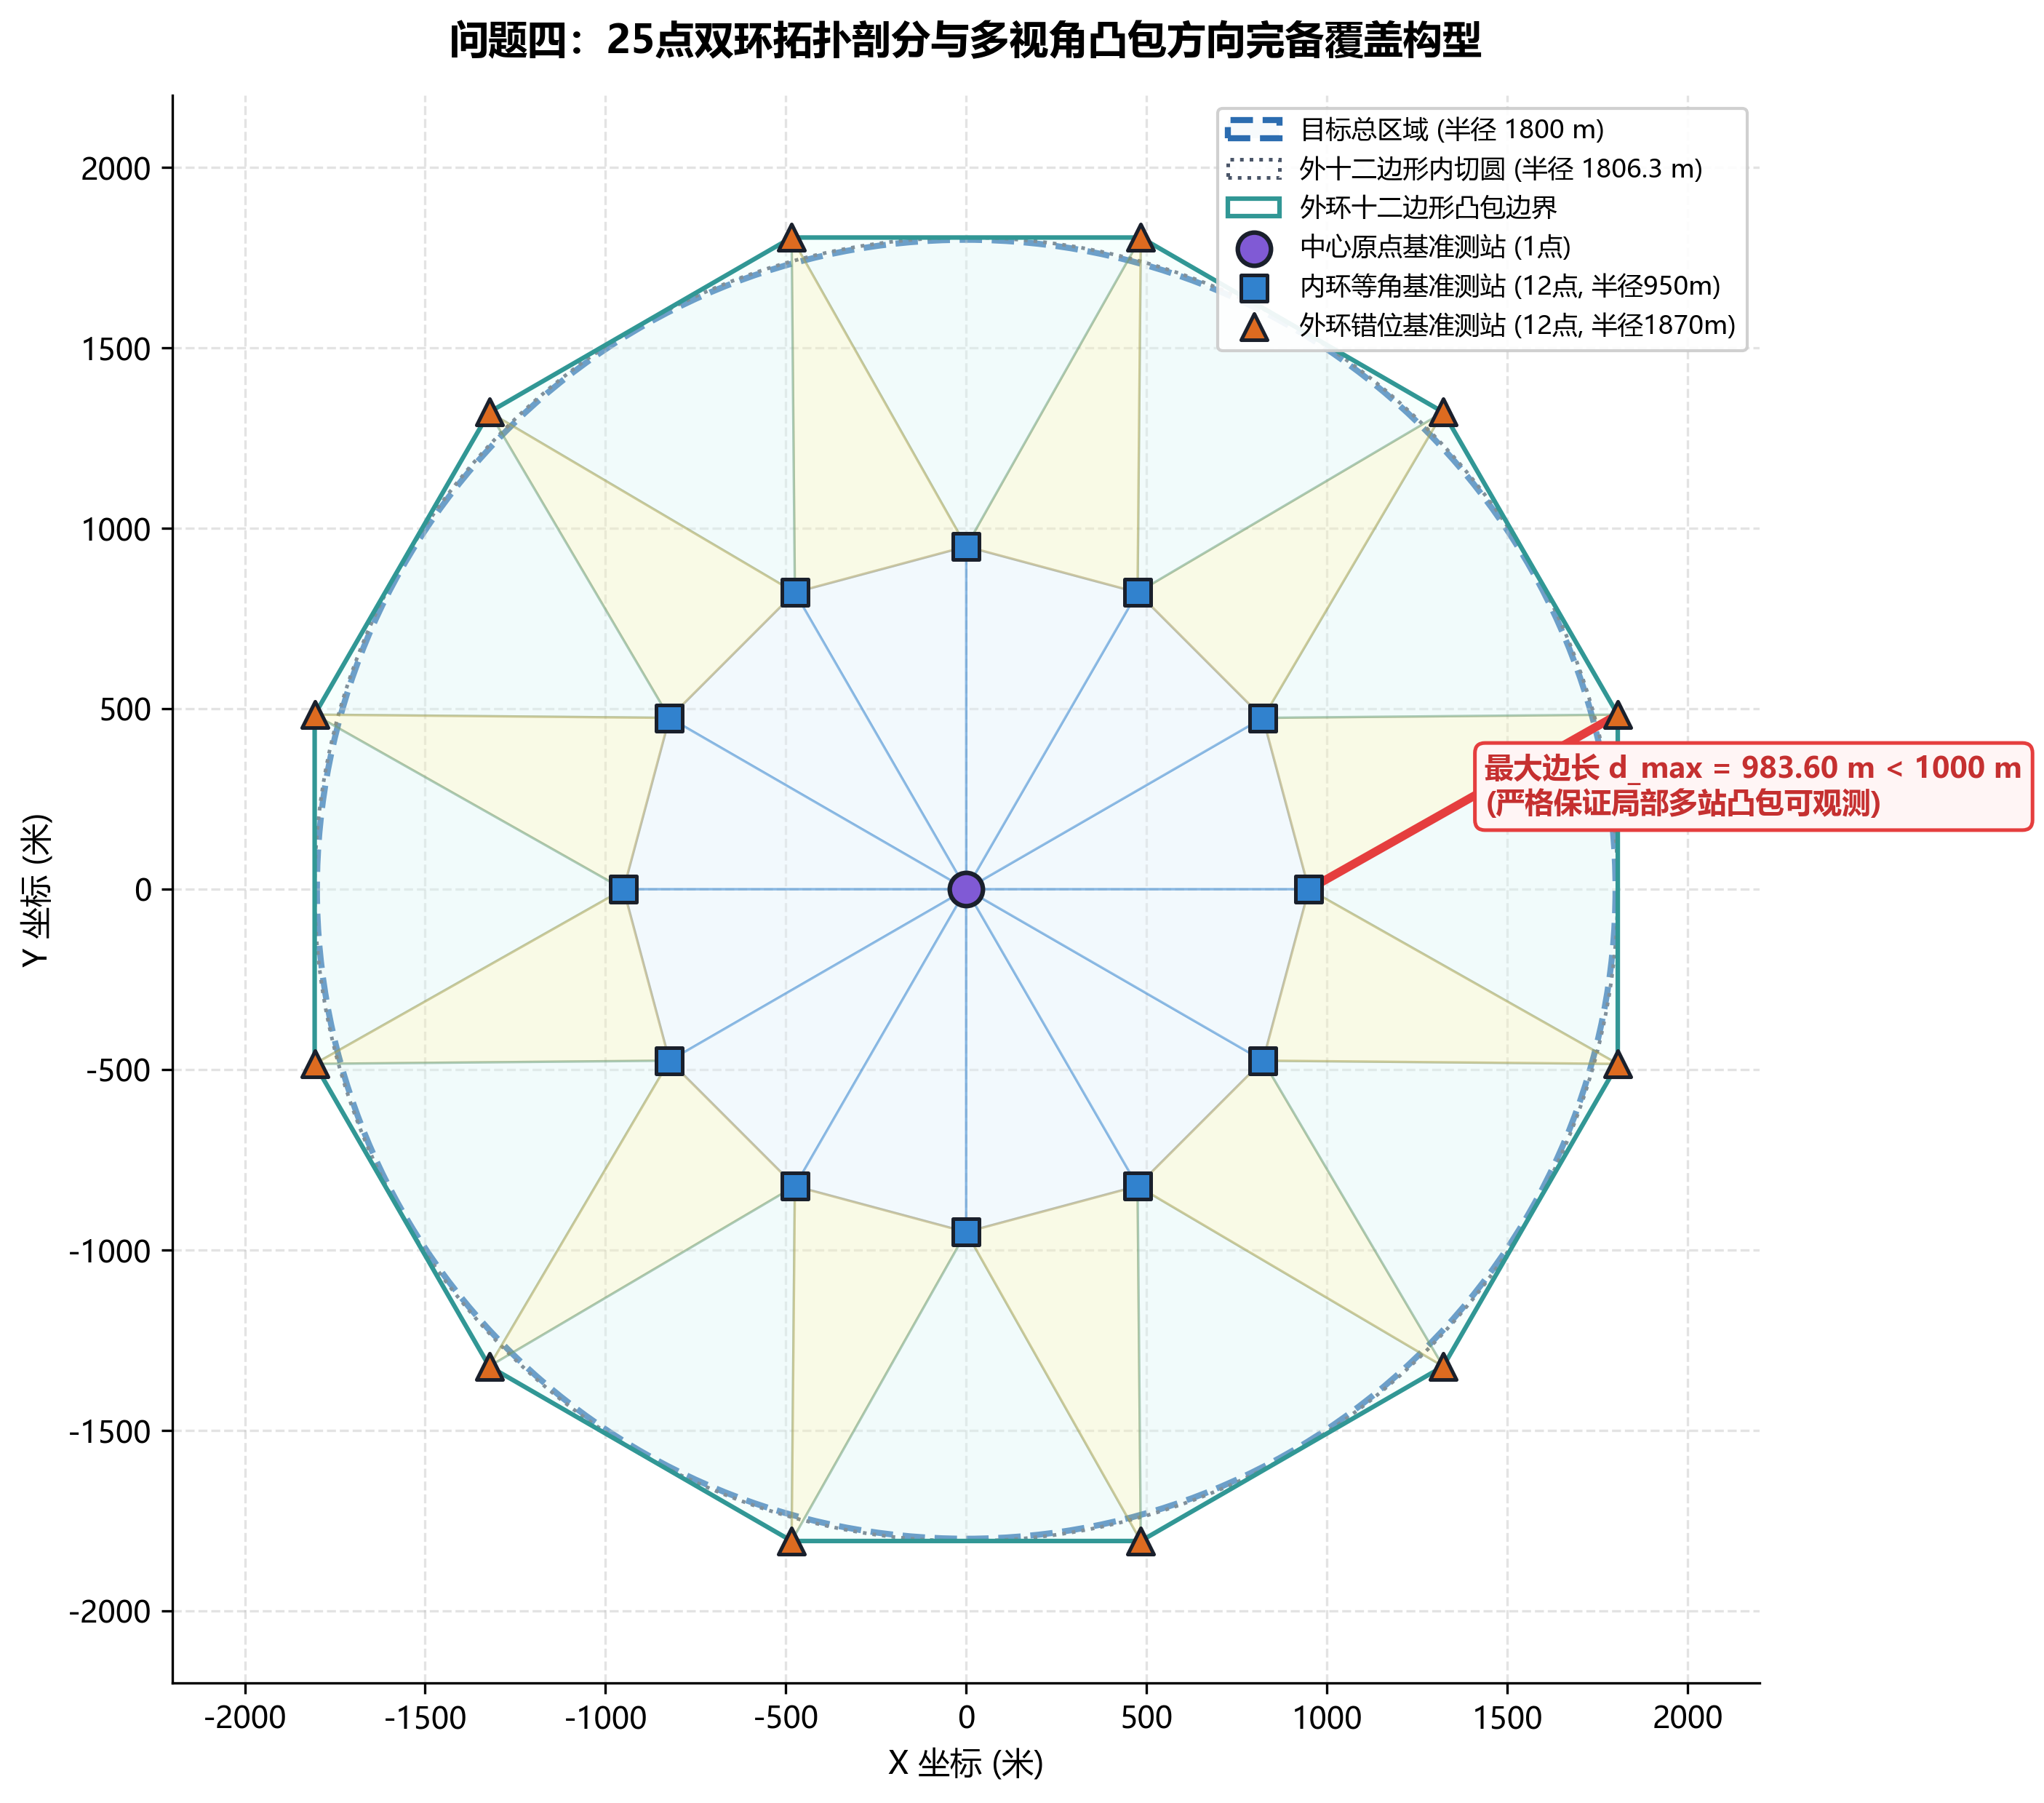
\includegraphics[width=0.60\linewidth]{images/fig_q4_25point_coverage.png}
    \vspace{-0.3em}
    \caption{25 点双环拓扑分布构型与机器狗双轨清除实测轨迹}
    \label{fig:q4_25point_coverage}
    \vspace{-0.3em}
\end{figure}

该网络共划分出 36 个三角形单元，单元边长涵盖四类连线：
\begin{enumerate}[leftmargin=2.2em, itemsep=0.02em, topsep=0.02em]
    \item 中心至内环边长：$d_1 = R_1 = 950\text{ m}$；
    \item 内环相邻边长：$d_2 = 2 R_1 \sin 15^\circ \approx 491.76\text{ m}$；
    \item 外环相邻边长：$d_3 = 2 R_2 \sin 15^\circ \approx 968.02\text{ m}$；
    \item 内外环跨接边长：$d_4 = \sqrt{R_1^2 + R_2^2 - 2 R_1 R_2 \cos 15^\circ} \approx 983.60\text{ m}$。
\end{enumerate}
所有单元的最长边满足 $d_{\max} = 983.60\text{ m} < 1000\text{ m}$。因此，区域内任意点所在的三角形三顶点，到该点的距离均小于 $1000\text{ m}$，且构成包含该点的闭凸包，满足推论 1 的可探测条件。此外，外环正十二边形内切圆半径为 $R_2 \cos 15^\circ \approx 1806.28\text{ m} > 1800\text{ m}$，实现了对目标区域的完全覆盖。

\begin{table}[htbp]
    \centering
    \footnotesize
    \vspace{-0.3em}
    \caption{25 点双环拓扑几何参数与方向完备验证表}
    \label{tab:q4_topology_params}
    \renewcommand{\arraystretch}{0.65}
    \setlength{\tabcolsep}{2.5pt}
    \begin{tabularx}{\linewidth}{l c c X}
        \toprule[1.5pt]
        \textbf{几何拓扑参数项} & \textbf{解析表达式 / 理论值} & \textbf{数值计算结果} & \textbf{全域探测保证判定结论} \\
        \midrule
        外环正十二边形内切圆半径 & $R_2 \cos(15^\circ) = 1870 \times 0.9659$ & $1806.28\text{ m}$ & 大于目标圆半径 $1800\text{ m}$，实现全域几何包络 \\
        剖分三角形最大边长 $d_{\max}$ & $\sqrt{R_1^2 + R_2^2 - 2 R_1 R_2 \cos(15^\circ)}$ & $983.60\text{ m}$ & 小于保底半径 $1000\text{ m}$，具备 $16.40\text{ m}$ 探测裕度 \\
        三角形单元几何顶点测距 & 任意内点至三顶点距离均 $\le d_{\max}$ & $\le 983.60\text{ m}$ & 每个单元内部点均能被其所在三角形 3 顶点有效覆盖 \\
        未知朝向多视角凸包判定 & 目标恒处于所在三角形三顶点闭凸包内 & 满足命题 5 条件 & 任意未知朝向至少落入一个顶点的有效视场内 \\
        \bottomrule[1.5pt]
    \end{tabularx}
\end{table}

\subsubsection{真值包含与安全选点}

25 点双环拓扑在宏观上保证了全域任意未知朝向的目标至少能被一个基准测站捕获。而在实际作业中，一旦机器狗在某一测站 $\mathbf{q}_1$ 处首次捕获频道 $c$ 的有效示向信号，系统便需要由全域巡航转入对该频道的交会定位。为确保后续多测站协同交会不丢失目标，首先必须保证交会多边形始终包含真实物理位置，且后续选点能够排除距离超距的混淆。

当在测站 $\mathbf{q}_1$ 处首次捕获频道 $c$ 的有效示向角 $\hat{\theta}_1$ 时，构建初始凸多边形位置外包：
\begin{equation}
    P_c^1 = P_{\Omega}^{\mathrm{out}} \cap \mathcal{B}^{\mathrm{out}}(\mathbf{q}_1, 1500) \cap \mathcal{W}(\mathbf{q}_1, \hat{\theta}_1, \varepsilon_{\mathrm{tol}})
\end{equation}
式中 $P_{\Omega}^{\mathrm{out}}$ 为目标区域的外切正多边形，$\mathcal{B}^{\mathrm{out}}$ 为测站最大覆盖圆的外切多边形，$\mathcal{W}$ 为示向角楔区域。在确定性测向误差界 $\varepsilon = 1^\circ$ 条件下，利用示向角楔持续求交可以不断压缩目标可行域，该多边形恒包含目标真实位置，具体由如下引理保证：

\noindent\textbf{引理 1（示向角交会多边形恒包含目标真实位置）}\quad 设初始外包满足 $\mathbf{x}_c \in P_c^1$。后续若仅采用有效示向角楔 $\mathcal{W}_k$ 进行半平面求交更新：
\begin{equation}
    P_c^{k+1} = P_c^k \cap \mathcal{W}_k
\end{equation}
则对任意步数 $k \ge 1$，均恒有 $\mathbf{x}_c \in P_c^k$。

引理 1 保证了只要测站获得有效示向角，交会多边形便能稳健收缩并锁定真实目标。然而，仅凭单次测向获得的角楔面积依然巨大，必须机动至第二测站进行双向交会。在定向天线半平面发射背景下，若第二测站与目标的距离超出覆盖半径 $R_c$，不仅无法接收信号，且系统无法区分未收到信号究竟是因为距离超距还是落入目标盲区。因此，第二检测点必须满足严格的距离安全准则，使无信号反馈不再受到距离超限因素的混淆。对于候选测站 $\mathbf{q}$，该准则要求其到多边形 $P_c^k$ 内任意可能目标位置的距离均不超过安全阈值。由于欧氏距离关于目标位置 $\mathbf{x}$ 为凸函数，上述最大距离可在顶点集 $\operatorname{Vert}(P_c^k)$ 上取得：
\begin{equation}
    d_{\max}(\mathbf{q}, P_c^k) = \max_{\mathbf{x} \in P_c^k} \|\mathbf{q} - \mathbf{x}\| = \max_{\mathbf{v} \in \operatorname{Vert}(P_c^k)} \|\mathbf{q} - \mathbf{v}\|
\end{equation}
算法筛选满足 $d_{\max}(\mathbf{q}, P_c^k) \le 995\text{ m}$ 的候选测站。由于 $995\text{ m} < 1000\text{ m} \le R_c$，这保证了测站对多边形内任意位置均在感知范围之内；此时若未收到信号，必为目标背向盲侧，而非距离超距。

\subsubsection{直接清除与网格遍历}

经过多测站交会收缩后，目标真实位置已被限定在紧致凸多边形 $P_c^k$ 内部。此时系统需要驱动机器狗实施物理清除，机载激光的有效清除半径为 $20\text{ m}$。若定位多边形已充分收缩，机器狗可停靠其最小外接圆圆心并直接清除目标；反之，若多边形仍然较大或主动测向预算已经耗尽，系统便转入无遗漏的网格遍历。为此，建立外接圆直接清除与正方形网格遍历相结合的双轨判定准则：

\noindent\textbf{判据 2（外接圆直接清除与正方形网格遍历条件）}\quad 针对频道 $c$ 的多边形可行域 $P_c^k$，采用 Welzl 算法计算其最小外接圆半径 $\rho(P_c^k)$ 及圆心 $\mathbf{c}_c$：
\begin{enumerate}[leftmargin=2.2em, itemsep=0.03em, topsep=0.03em]
    \item \textbf{常规定位提前清除}：若 $\rho(P_c^k) \le 19.5\text{ m}$，机动至 $\mathbf{c}_c$ 实施激光清除。其中 $20.0\text{ m}$ 为题目规定的有效清除半径，采用 $19.5\text{ m}$ 作为提前判定阈值，预留 $0.5\text{ m}$ 数值稳健裕量；
    \item \textbf{尾部探测后清除}：在完成最后一次尾部追加探测后，若后验外接圆半径满足充分清除界 $\rho(P_c^{k+1}) \le 20.0\text{ m}$，直接机动至新圆心实施清除；
    \item \textbf{网格遍历清除}：若未达上述条件，对 $P_c^k$ 的外接水平矩形作边长 $\Delta g = 26\text{ m}$ 正方形网格划分，完整保留所有与 $P_c^k$ 相交的单元，沿蛇形次序依次遍历各相交单元中心实施清除。
\end{enumerate}

为证明网格遍历策略在几何上绝不会发生遗漏，给出如下单元覆盖保证：

\noindent\textbf{引理 2（相交正方形网格遍历对目标的覆盖保证）}\quad 边长为 $\Delta g = 26\text{ m}$ 的正方形网格单元中，中心点至单元内任意点的最大距离为：
\begin{equation}
    r_{\mathrm{cell}} = \frac{\sqrt{2}}{2} \Delta g \approx 18.385\text{ m} < 20.0\text{ m}
\end{equation}
因该距离严格小于激光清除半径，机器狗只需停靠各相交网格中心执行清除，即可完全覆盖对应单元。只要目标位于相交网格并集内，有限步遍历必能完成清除。

\subsubsection{全局终止判定}

前述命题与引理保证了任意单个目标从被发现、定位到物理清除的完整过程。然而，在全自主作业背景下，全场客观存在的目标总数未知（在 10 至 16 之间随机），且机器狗并不知道具体哪些频道存在目标。为了避免盲目过早停工造成漏检，同时防止全场目标清除完毕后陷入无效空转，系统必须建立全局可判定的自主退出准则：

\noindent\textbf{准则 3（混合干扰源全域搜索终止与退出条件）}\quad 当满足以下任一条件时，系统终止搜索任务并安全退出：
\begin{enumerate}[leftmargin=2.2em, itemsep=0.03em, topsep=0.03em]
    \item \textbf{目标数量达上限}：累计清除的目标频道数达到理论上限 $|\mathcal{C}^{\mathrm{clear}}| = 16$；
    \item \textbf{全频道检测完成}：所有已发现的目标均已完成清除，且其余未发现目标的频道在 25 个基准测站的检测中均明确返回 $\texttt{no\_signal}$，即满足 $\forall c \in \mathcal{C}, c \in \mathcal{C}^{\mathrm{clear}} \lor [ \mathcal{M}_c = \{1, \dots, 25\} \land \forall i \in \{1, \dots, 25\}, y_{c,i} = \texttt{no\_signal} ]$。若通信超时或响应未知，不得计入无信号。
\end{enumerate}

\subsection{在线策略与算法}

第 6.3 节建立的 25 点基准拓扑、距离安全交会与网格遍历构成了确保 100\% 清除的理论保证主链。然而，若系统单纯依赖基准测站巡航与大范围网格遍历，一旦在第二测站遇到定向盲侧便直接退化为网格扫描，将消耗过多的机动与清除时间。因此，本文在理论保证主链之外增加两条轻量决策支路 \cite{bercea2016}：盲侧失联时尝试对称镜像探测，定位多边形仍较大时评估尾部追加探测的预期收益。两项机制在不改变完全清除保证主链的前提下，用于显著压缩任务总时间。

\subsubsection{镜像探测与自适应尾部探测}

若测站对当前外包多边形满足安全距离条件（$d_{\max} \le 995\text{ m}$），但实测明确返回无信号，则可判定测站处于定向目标的辐射盲侧。针对该情况，设计两项优化机制：
\begin{enumerate}[leftmargin=2.2em, itemsep=0.04em, topsep=0.03em]
    \item \textbf{条件对称镜像探测}：若主动测向预算尚未耗尽，算法沿首次示向中轴线将失联测站对称反射至对侧几何位置：
    \begin{equation}
        \mathbf{q}_{\mathrm{mirror}} = \mathbf{q}_1 + 2 \big[ (\mathbf{q}_2 - \mathbf{q}_1)^\top \mathbf{u}(\hat{\theta}_1) \big] \mathbf{u}(\hat{\theta}_1) - (\mathbf{q}_2 - \mathbf{q}_1)
    \end{equation}
    重新校验顶点距离安全后前往探测，增加落入有效发射半平面的概率。
    \item \textbf{自适应尾部追加探测}：在当前多边形内离散生成 96 个位置与 36 个法向朝向样本，筛选相容于历史观测的样本子集 $\mathcal{H}_k$。定义候选测站的相容状态比例：
    \begin{equation}
        p_v(\mathbf{q}) = \frac{\#\{(\mathbf{x}_i, \mathbf{u}_j) \in \mathcal{H}_k \mid \mathbf{q} \text{ 对该状态满足可接收条件}\}}{\#\mathcal{H}_k} \in [0, 1]
    \end{equation}
    若 $\mathcal{H}_k = \emptyset$，则不触发追加探测。
\end{enumerate}

综合上述收益与代价量化关系，自适应尾部追加探测的触发判据确立如下：

\noindent\textbf{判据 3（尾部探测收益代价判定条件）}\quad 记网格遍历预估耗时为 $T_{\mathrm{grid}}$，候选点探测耗时为 $T_{\mathrm{probe}} = d/v + 5\text{ s} + \mathbb{I}_{\mathrm{switch}} \times 1\text{ s}$（$\mathbb{I}_{\mathrm{switch}}$ 为切频指示）。定义非空相交示向集以及探测后的后验最大可能直径：
\begin{equation}
    \Theta_k^+(\mathbf{q}) = \big\{\theta \in \Theta_{\mathrm{sample}} \mid P_c^k \cap \mathcal{W}(\mathbf{q}, \theta, \varepsilon_{\mathrm{tol}}) \neq \emptyset\big\}
\end{equation}
\begin{equation}
    D_{\mathrm{post}} = \max_{\theta \in \Theta_k^+(\mathbf{q})} \operatorname{diam}\big(P_c^k \cap \mathcal{W}(\mathbf{q}, \theta, \varepsilon_{\mathrm{tol}})\big)
\end{equation}
若 $\Theta_k^+(\mathbf{q}) = \emptyset$ 则不触发探测。当相容比例满足 $p_v \ge 0.30$，且预估时间收益高于机动探测代价时，执行追加探测：
\begin{equation}
    T_{\mathrm{probe}} < T_{\mathrm{grid}} \cdot p_v \left[ 1 - \left( \frac{D_{\mathrm{post}}}{D} \right)^2 \right]
\end{equation}
探测后的分支处理规则如下：
\begin{enumerate}[leftmargin=2.2em, itemsep=0.03em, topsep=0.02em]
    \item 若返回 $\texttt{near}$，直接在当前位置执行激光清除；
    \item 若获取有效示向，更新位置外包。若后验外接圆半径满足 $\rho(P_c^{k+1}) \le 20.0\text{ m}$ 则直接清除，否则转入 26 米网格遍历；
    \item 若再次返回 $\texttt{no\_signal}$ 或判据不满足，直接转入 26 米网格遍历清除。
\end{enumerate}

\subsubsection{系统架构与算法流程}

系统协同架构如图 \ref{fig:q4_system_architecture} 所示，全向与定向混合干扰源搜索、补充探测与清除流程如图 \ref{fig:q4_flowchart} 所示，算法流程汇总于表 \ref{tab:q4_algorithm}。

\begin{figure}[htbp]
    \centering
    \vspace{-0.2em}
    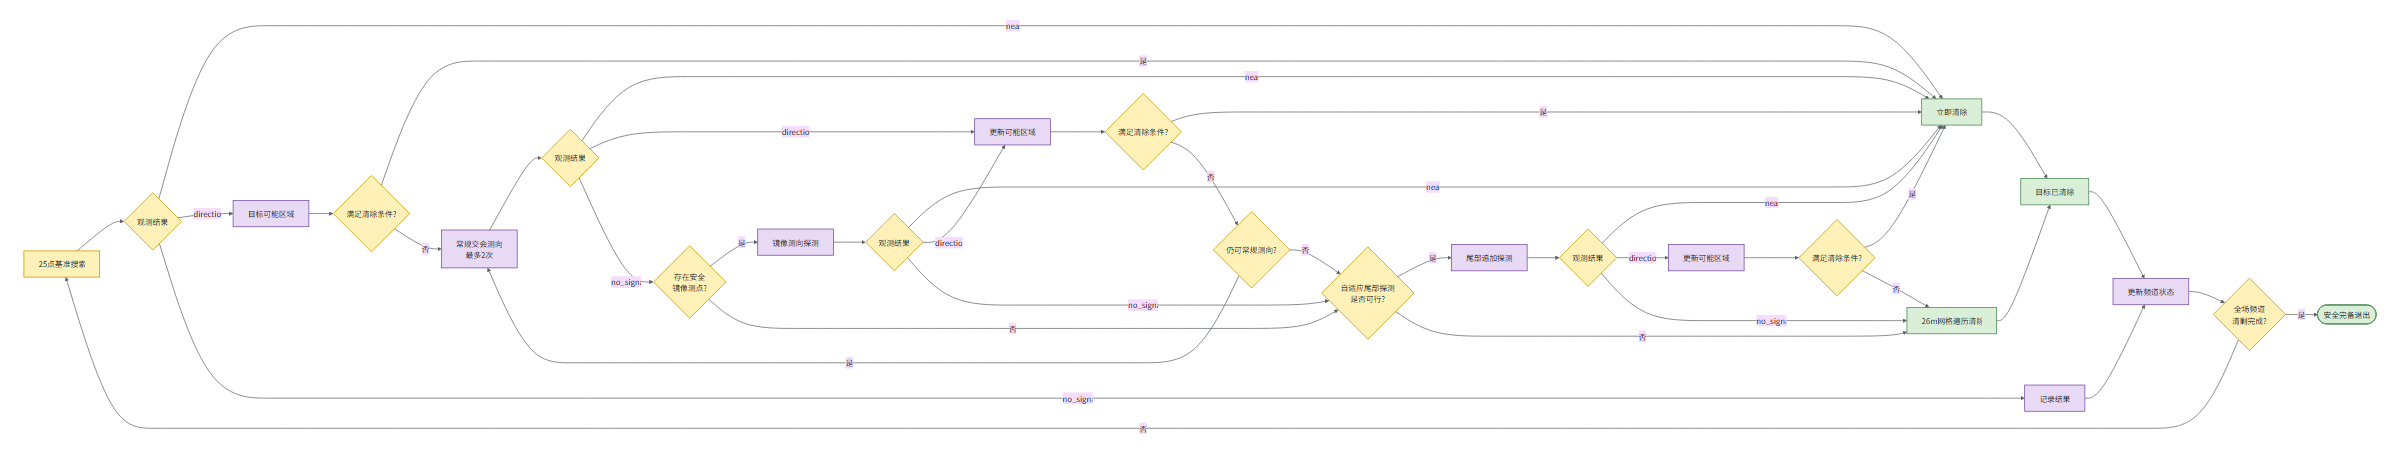
\includegraphics[width=0.98\linewidth]{images/fig_q4_flowchart.png}
    \vspace{-0.3em}
    \caption{全向与定向混合干扰源搜索、补充探测与清除流程}
    \label{fig:q4_flowchart}
    \vspace{-0.3em}
\end{figure}

\begin{figure}[htbp]
    \centering
    \vspace{-0.2em}
    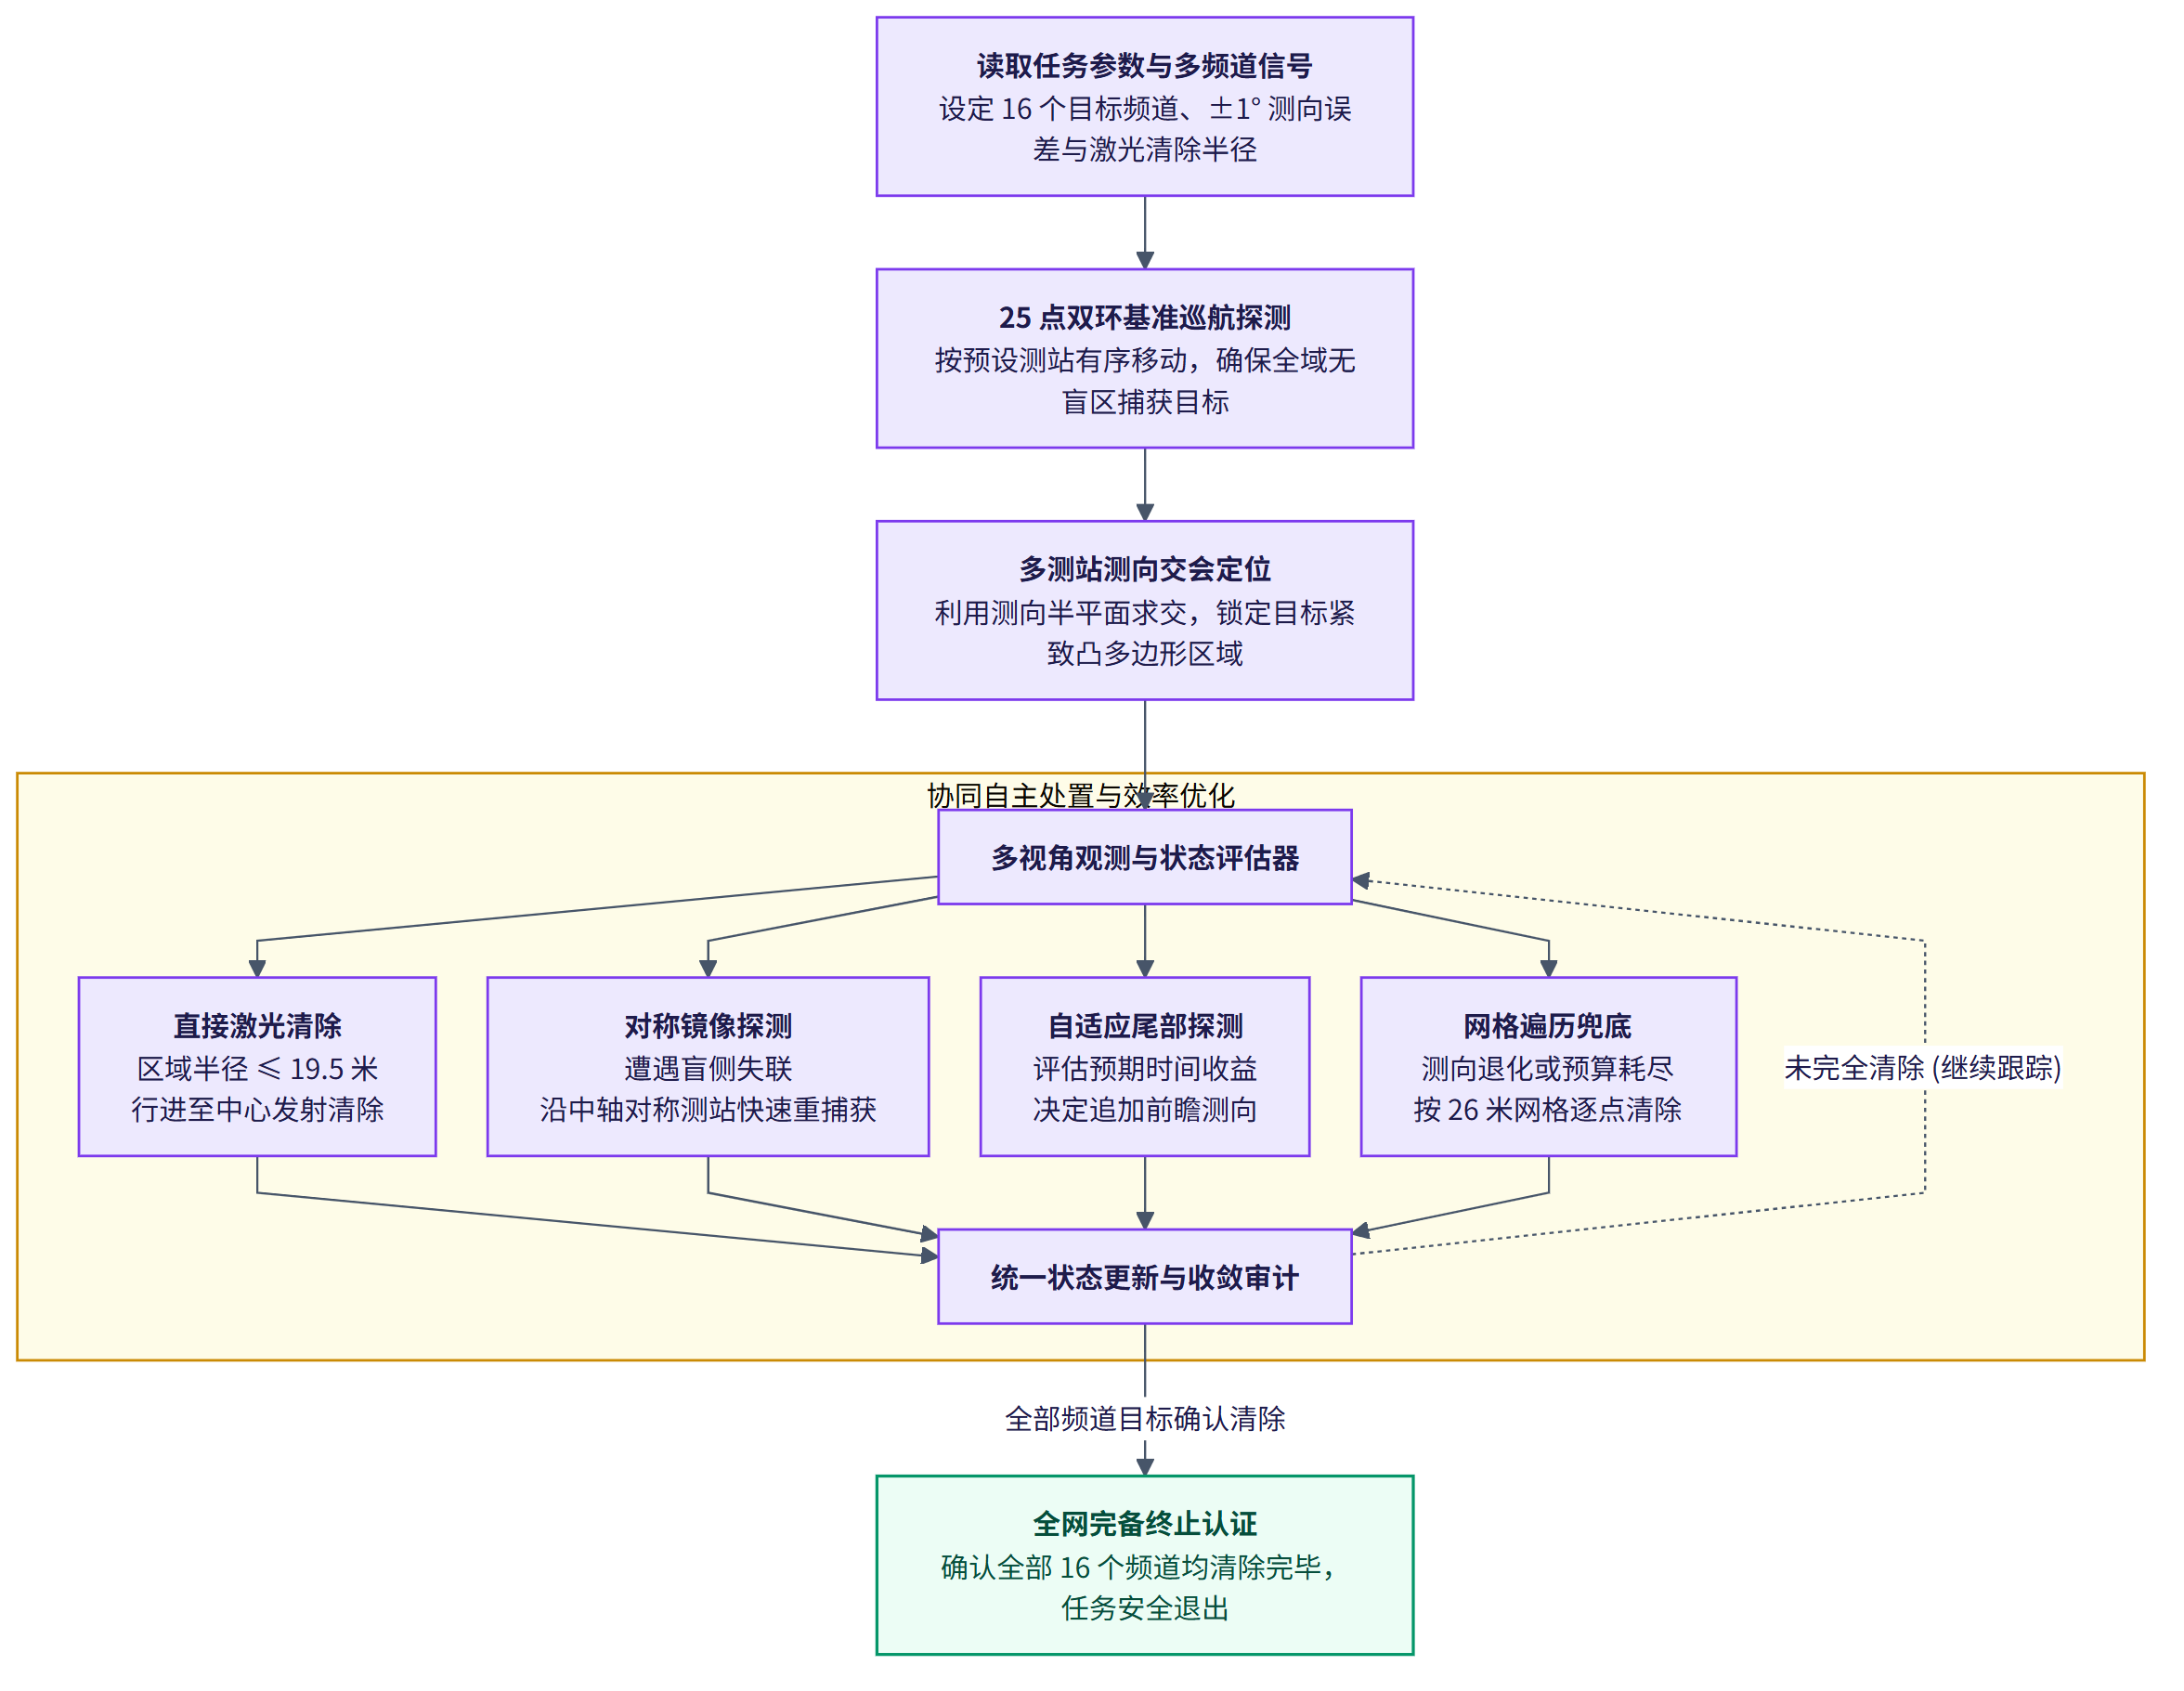
\includegraphics[width=0.98\linewidth]{images/fig_q4_system_architecture.png}
    \vspace{-0.3em}
    \caption{全向—定向混合干扰源自主协同搜索与清除系统架构图}
    \label{fig:q4_system_architecture}
    \vspace{-0.3em}
\end{figure}

\begin{table}[htbp]
    \centering
    \footnotesize
    \vspace{-0.3em}
    \caption{混合干扰源多视角搜索与清除算法流程表}
    \label{tab:q4_algorithm}
    \renewcommand{\arraystretch}{0.65}
    \begin{tabularx}{\linewidth}{l X}
        \toprule[1.5pt]
        \multicolumn{2}{l}{\textbf{算法 2：} 基于多视角拓扑包围与自适应尾部探测的混合干扰源清除算法} \\
        \midrule
        \textbf{输入：} & 目标区域 $\Omega$，25 点双环拓扑 $\mathcal{S}_{25}$，物理动作时间模型，主动测向预算 $N_{\mathrm{loc\_max}}=2$ \\
        \textbf{输出：} & 机器狗动作序列，目标清除记录表，任务总虚拟时间 $T_{\mathrm{virtual}}$ \\
        步骤 1 & 初始化位姿 $\mathbf{p}_0 = (0,0)$，频道信息状态 $\mathcal{I}_c^0$，规划 25 点基准搜索测站巡航次序； \\
        步骤 2 & 检查准则 3 退出条件：若满足则结束任务并输出报告，否则进入主调度循环； \\
        步骤 3 & 优先检查是否存在满足直接清除条件频道（$\rho \le 19.5\text{ m}$）：若存在则机动至圆心实施清除； \\
        步骤 4 & 从主动测向次数少于 2 次的定位中频道中选择目标，并在满足 $d_{\max} \le 995\text{ m}$ 的候选测站中确定下一测点。完成测向后，若返回 $\texttt{near}$，则在当前位置直接清除；若获得有效示向，则求交裁剪并更新外包；若返回 $\texttt{no\_signal}$，则评估对称镜像测站； \\
        步骤 5 & 对仍未收敛的频道评估判据 3。若满足尾部探测条件，则追加一次测向：返回 $\texttt{near}$ 时直接清除；获得有效示向且 $\rho \le 20.0\text{ m}$ 时直接清除；其余情况转入网格遍历。若判据不满足，则直接遍历与当前外包相交的网格； \\
        步骤 6 & 若无待处理定位频道，沿基准拓扑机动至下一基准测站，扫描未结案频道； \\
        步骤 7 & 接收物理动作反馈，单向更新频道状态、凸多边形外包及 25 点检测记录，返回步骤 2； \\
        \bottomrule[1.5pt]
    \end{tabularx}
\end{table}

\subsubsection{完全清除与终止性分析}

算法 2 将全域基准拓扑巡航、距离安全交会、自适应效率支路与网格遍历有机融为一体。为验证该系统在理论上绝不会发生死循环、漏检或无限震荡，下面结合引理 1、引理 2 与准则 3，证明该清除过程必在有限个离散动作步内终止：

\noindent\textbf{命题 6（混合干扰源搜索清除过程有限步终止）}\quad 在目标静止、总数不超过 16 个且测向误差在确界内的物理假设下，算法 2 必在有限个离散动作步数内完成全部实际存在目标的清除并安全退出。

\begin{cumcmproof}
在搜索清除任务全过程中，系统可生成的离散决策动作总量存在有限确定上界：
\begin{enumerate}[leftmargin=2.2em, itemsep=0.03em, topsep=0.02em]
    \item \textbf{基准搜索任务有限}：25 个基准测站对 20 个频道的巡航扫描总次数至多为 $25 \times 20 = 500$ 次；
    \item \textbf{主动探测任务有限}：实际目标至多 16 个，每个目标常规主动测向至多 2 次、尾部探测至多 1 次；
    \item \textbf{网格清除任务有限}：根据引理 1，目标真实位置恒包含于凸多边形外包内；由于外包多边形有界，其相交的 26 米正方形网格单元数必然有限，且每个单元中心至多访问清除 1 次。
\end{enumerate}
算法按照固定优先级次序逐一推进待定位与待清除频道，每一步动作均单调消耗待处理任务集，不存在死循环与状态回退，因此算法必在有限离散步数内完成全部实际存在目标的清除并满足准则 3 退出条件。证毕。
\end{cumcmproof}

\subsection{测试结果与分析}

\subsubsection{本地配对实验}

为检验自适应尾部追加探测对缩减任务耗时的具体作用，在 100 组随机生成的同分布场景（随机种子 0 至 99）下开展同场景配对对比实验，对比未启用尾部探测的方案（V2）与本文完整方案（V3）。统计数据汇总于表 \ref{tab:q4_ablation_results}。

\begin{table}[htbp]
    \centering
    \footnotesize
    \vspace{-0.3em}
    \caption{V2 与 V3 算法在 100 组配对场景下的对比实验表}
    \label{tab:q4_ablation_results}
    \renewcommand{\arraystretch}{0.65}
    \setlength{\tabcolsep}{2.5pt}
    \begin{tabularx}{\linewidth}{l c c X}
        \toprule[1.5pt]
        \textbf{评估指标项} & \textbf{未启用尾部探测方案 (V2)} & \textbf{本文完整方案 (V3)} & \textbf{配对测试增益分析} \\
        \midrule
        全场景目标清除率 & 100\%（100 / 100 场） & 100\%（100 / 100 场） & 保持 100\% 完备清除底线 \\
        全任务虚拟总时间均值 & $7323.1\text{ s}$ & $7213.3\text{ s}$ & 配对平均缩减 $109.8\text{ s}$ \\
        虚拟总时间 95\% 置信区间 & $[7148.2, 7498.0]\text{ s}$ & $[7042.8, 7383.8]\text{ s}$ & 均值差配对区间 $[-158.7, -60.9]\text{ s}$ \\
        样本最劣场景任务总时间 & $10094.6\text{ s}$（种子 43） & $9448.1\text{ s}$（种子 43） & 样本最劣工况耗时减少 $646.5\text{ s}$ \\
        单场平均无效清除尝试次数 & $46.78\text{ 次}$ & $27.99\text{ 次}$ & 无效网格遍历减少 40.2\% \\
        逐案例耗时胜平负统计分布 & 基准方案低 6 场 & 本文方案低 35 场 & 59 场耗时相同 \\
        \bottomrule[1.5pt]
    \end{tabularx}
\end{table}

实验数据表明，在 100 组配对样本中，两种方案目标清除率均达到 100\%；V3 相对 V2 耗时降低、相同和升高的场数分别为 35、59 和 6；全场平均无效清除尝试由 46.78 次降至 27.99 次，样本集中最长耗时减少 $646.5\text{ s}$。

\subsubsection{演练与正式测试结果}

在接入比赛官方评测环境的连续批次中，算法进行了 17 轮全流程实测演练，检验在不同目标数目（涵盖 $10\sim 16$ 个各档位）下的运行指标，实测数据汇总于表 \ref{tab:q4_rehearsal_summary}。

\begin{table}[htbp]
    \centering
    \footnotesize
    \vspace{-0.3em}
    \caption{17 轮真实接口规范演练测试结果汇总表}
    \label{tab:q4_rehearsal_summary}
    \renewcommand{\arraystretch}{0.65}
    \setlength{\tabcolsep}{2.5pt}
    \begin{tabular*}{\linewidth}{@{\extracolsep{\fill}}l c c c c c}
        \toprule[1.5pt]
        \textbf{演练测试轮次区间} & \textbf{测试场次} & \textbf{累计清除源数} & \textbf{全场清除率} & \textbf{加权平均单源耗时} & \textbf{单源耗时中位数} \\
        \midrule
        少目标工况（$10\sim 11$ 源） & 4 场 & 42 个 & 100\% & $612.8\text{ s/源}$ & $598.2\text{ s/源}$ \\
        中目标工况（$12\sim 14$ 源） & 8 场 & 104 个 & 100\% & $523.4\text{ s/源}$ & $496.5\text{ s/源}$ \\
        多目标工况（$15\sim 16$ 源） & 5 场 & 75 个 & 100\% & $493.6\text{ s/源}$ & $481.0\text{ s/源}$ \\
        \midrule
        \textbf{17 轮全演练总体汇总} & \textbf{17 场} & \textbf{221 个} & \textbf{100\%} & \textbf{530.41 s/源} & \textbf{502.43 s/源} \\
        \bottomrule[1.5pt]
    \end{tabular*}
\end{table}

实测表明，在累计 221 个未知全向与定向混合目标中，系统清除率达到 100\%。按照赛题规范要求，针对未知混合干扰源开展三次正式测试，实测结果汇总于表 \ref{tab:q4_official_tests}。三次测试共清除 38 个目标（清除率 100\%），单源平均定位清除时间分别为 $559.214\text{ s}$、$586.146\text{ s}$ 与 $466.809\text{ s}$，加权均值达 $533.675\text{ s/源}$。

\begin{table}[htbp]
    \centering
    \footnotesize
    \vspace{-0.3em}
    \caption{赛题规范三次测试结果记录表}
    \label{tab:q4_official_tests}
    \renewcommand{\arraystretch}{0.75}
    \setlength{\tabcolsep}{3.0pt}
    \begin{tabular*}{\linewidth}{@{\extracolsep{\fill}}l c c c c}
        \toprule[1.5pt]
        \textbf{正式测试案例编码} & \textbf{清除目标数量} & \textbf{平均定位清除时间 / s} & \textbf{虚拟任务总时间 / s} & \textbf{程序算法运行时间 / s} \\
        \midrule
        \texttt{4Z33-SF8B-2CGX-7UYM} & 12 个 & 559.214 & 6710.566 & 5.546 \\
        \texttt{MAF3-M9C7-BEAZ-D6V9} & 12 个 & 586.146 & 7033.752 & 6.100 \\
        \texttt{KKFA-B32Q-ZKTZ-ETUB} & 14 个 & 466.809 & 6535.328 & 6.046 \\
        \midrule
        \textbf{汇总 / 加权均值} & \textbf{38 个} & \textbf{533.675} & \textbf{6759.882} & \textbf{5.897} \\
        \bottomrule[1.5pt]
    \end{tabular*}
\end{table}


\section{模型评价、改进与推广}

\subsection{模型优点}
\begin{enumerate}[leftmargin=2.2em, itemsep=0.01em, topsep=0.01em]
    \item \textbf{几何覆盖保障与数理推导}：不依赖目标先验分布假设，基于平面几何凸包包含定理与极值分离性质，构建完备覆盖与真值包含关系；
    \item \textbf{保证主链与效率支路协同分工}：以基准多视角覆盖和有限网格遍历承担完备清除保证，以距离安全探测和尾部探测优化动作次序；
    \item \textbf{计算效率与在线实测表现}：Q3 三次正式测试的程序运行时间均值为 $4.215\text{ s}$，Q4 为 $5.897\text{ s}$，均远低于 $1200\text{ s}$ 的程序运行上限；100 组本地重复测试、100 组 Q4 配对实验与正式测试共同记录了当前实现的运行表现。
\end{enumerate}

\subsection{模型局限与改进}
\begin{enumerate}[leftmargin=2.2em, itemsep=0.01em, topsep=0.01em]
    \item \textbf{极端多径退化对多边形求交的数值扰动}：当极端测量噪声导致测向角域畸变时，半平面求交可能出现微小退化多边形，需进一步增强近退化边界的自适应拓扑容差修复机制。
    \item \textbf{通信异常恢复状态机仍需增强}：当前模型假设通信偶发中断单次重试成功，若出现长时间信道离线且服务端事务未决，需进一步补充本地持久化恢复协议。
\end{enumerate}

\subsection{模型推广}
本文建立的多视角凸包覆盖与误差集交会决策方法，可推广应用于：
\begin{enumerate}[leftmargin=2.2em, itemsep=0.01em, topsep=0.01em]
    \item 复杂电磁环境下的无人地面平台自主搜寻与干扰源定位；
    \item 具有半平面辐射特性与角度测向约束的地面无线电信标协同搜索；
    \item 有限视场角约束下的多移动机器人协同搜索与环境信标定位。
\end{enumerate}

\section*{AI工具使用声明}
本参赛队在竞赛过程中使用了人工智能（AI）工具，主要用于论文排版语法检查、可视化绘图代码调试与部分文字措辞润色，详细使用情况见支撑材料《AI工具使用详情.pdf》。本论文的核心数学建模、公式推导、算法求解及数值分析均由本参赛队三位队员独立主导完成，并对全篇内容进行了完整的人工核验。

\begin{thebibliography}{99}
\setlength{\itemsep}{-1.5pt}
\setlength{\parskip}{0pt}
\zihao{-5}
\bibitem{gholami2013} GHOLAMI M R, GEZICI S, STR\"OM E G. Worst-case positioning error and sensor placement for range-difference based localization[J]. IEEE Transactions on Signal Processing, 2013, 61(14): 3532-3546.
\bibitem{toussaint1983} TOUSSAINT G T. Solving geometric problems with the rotating calipers[C]//Proceedings of IEEE MELECON '83. Athens: IEEE, 1983: 1-8.
\bibitem{welzl1991} WELZL E. Smallest enclosing disks (balls and ellipsoids)[M]//New Results and New Trends in Computer Science. Berlin: Springer, 1991: 359-370.
\bibitem{tokekar2013} TOKEKAR P, ISLER V. Sensor placement and selection for bearing sensors with bounded uncertainty[C]//IEEE International Conference on Robotics and Automation (ICRA). Karlsruhe: IEEE, 2013: 2515-2520.
\bibitem{dogancay2008} DO\u{G}AN\c{C}AY K, HMAM H. Optimal angular sensor separation for AOA localization[J]. Signal Processing, 2008, 88(3): 648-660.
\bibitem{vanderhook2014} VANDER HOOK P, TOKEKAR P, ISLER V. Cautious greedy strategy for active localization with bounded-error sensors[C]//IEEE/RSJ International Conference on Intelligent Robots and Systems (IROS). Chicago: IEEE, 2014: 4320-4325.
\bibitem{choset2001} CHOSET H. Coverage for robotics: A survey of recent results[J]. Annals of Mathematics and Artificial Intelligence, 2001, 31(1): 113-126.
\bibitem{song2012} SONG D, KIM C Y, YI J. Simultaneous localization of multiple unknown and transient radio sources using a mobile robot[J]. IEEE Transactions on Robotics, 2012, 28(3): 668-680.
\bibitem{guvensan2011} GUVENSAN M A, YAVUZ A G. On coverage issues in directional sensor networks: A survey[J]. Computer Networks, 2011, 55(15): 3358-3378.
\bibitem{bercea2016} BERCEA I O, ISLER V, KHULLER S. Minimizing uncertainty through sensor placement with angle constraints[C]//Proceedings of the 28th Canadian Conference on Computational Geometry (CCCG). Vancouver: Simon Fraser University, 2016: 28-34.
\end{thebibliography}

\end{document}
